\documentclass[12pt]{article}
% Some custom commands to make typing easier. Feel free to add to it


% quick homomorphism
\newcommand{\homo}[1]{\varphi (#1)}
% quick inverse
\newcommand{\inv}[1]{#1^{-1}}
% quick generating set
\newcommand{\genset}[1]{\langle #1 \rangle}
% split problem into multiple parts
\newcommand{\spl}{\rule{\textwidth}{0.4pt}}
% quick normal subgroup
\newcommand{\nsub}{\trianglelefteq}
% quick Z/nZ
\newcommand{\znz}[1]{\mathbb{Z\text{/#1}Z}}
% quick stirling numbers
% \newcommand{\squig}{\genfrac{\lbrace}{\rbrace}{0pt}{}}
\newcommand{\squig}[2]{\left\{{#1 \atop #2}\right\}}


% quick projective surface
\newcommand{\proj}[1]{\mathbb P^{#1}(\mathbb C)}
% quick elliptic curve
\newcommand{\ellip}{E(\mathbb{C})}
% quick ramification
\newcommand{\ram}[1]{e_{#1}}

% todo list
\usepackage[color=yellow]{todonotes}
\newcommand{\tbd}[1]{\todo[inline]{#1}
\addcontentsline{toc}{subsubsection}{TODO}}

% scaling tikz
\usepackage{adjustbox}

% format bullets
% \usepackage[shortlabels]{enumitem}

% Document inherent packages to be loaded
\usepackage{amsmath, amsfonts, amssymb, amsthm, graphicx, url, xcolor, enumerate, tcolorbox}

%geometry helps manage margins, among other things.
\usepackage[rmargin=2in,lmargin=1in,tmargin=1in,bmargin=1in]{geometry}
\newcommand{\sidenote}[1]{\marginpar{\footnotesize \begin{itemize}
    \item[$\leftarrow$]\raggedright #1
\end{itemize}}}

\setlength{\headheight}{16pt}
\setlength{\marginparwidth}{1.5in}
\makeatletter      % make title smaller   
\def\@maketitle{   % custom maketitle 
\begin{center}
    {\Large \@title} \\[0.1in] \@author \\ {\small \@date}
\end{center}  
}
\setcounter{secnumdepth}{0}

% new color for the hypers
\definecolor{hyperpurp}{RGB}{108,113,196}
\usepackage[colorlinks = true,
            linkcolor = hyperpurp,
            urlcolor  = hyperpurp,
            citecolor = hyperpurp,
            anchorcolor = hyperpurp]{hyperref}

\usepackage[all,2cell,ps]{xy}
\usepackage{tikz, tikz-cd}
\usepackage{faktor}
\allowdisplaybreaks
\graphicspath{{Images/}}

\theoremstyle{definition}  % to get rid of the italics
\newtheorem{theorem}{\bt{Theorem}}%[section]
\newtheorem{proposition}[theorem]{\bt{Proposition}}
\newtheorem{corollary}[theorem]{\gt{Corollary}}
\newtheorem{lemma}[theorem]{\bt{Lemma}}
\newtheorem{conjecture}[theorem]{Conjecture}

\newtheorem{defn}{\rt{Definition}}

\newtheorem{eg}{\textcolor{violet}{Example}}
\newtheorem{cautiouseg}[eg]{\textcolor{magenta}{Tricky example}}
\newtheorem{noneg}[eg]{\textcolor{violet}{Non-example}}

\newtheorem*{rmk}{Remark}


%Import the natbib package and sets a bibliography  and citation styles
\usepackage{natbib}

% Create headers
\usepackage{fancyhdr}
\usepackage{xcolor}
\renewcommand{\headrulewidth}{0pt}
\fancypagestyle{updated}{%
    \fancyhead{MATH103 Notes \hfill\hfill Xuehuai He}
    \fancyfoot{\hyperlink{toc}{Back to TOC}\hfill\thepage \hfill \textcolor{lightgray}{\today}}
}

% \newcommand{\Belyi}{Bely\u{\i}~}
% \newcommand{\thm}[3]{\vskip 0.2in \begin{center} \fbox{\begin{minipage}{0.8\linewidth} \begin{theorem}[#1] \label{#2} #3 \end{theorem} \end{minipage}} \end{center} \vskip 0.2in}
% \newcommand{\prop}[3]{\vskip 0.2in \begin{center} \fbox{\begin{minipage}{0.8\linewidth} \begin{proposition}[#1] \label{#2} #3 \end{proposition} \end{minipage}} \end{center} \vskip 0.2in}
% \newcommand{\cor}[3]{\vskip 0.2in \begin{center} \fbox{\begin{minipage}{0.8\linewidth} \begin{corollary}[#1] \label{#2} #3 \end{corollary} \end{minipage}} \end{center} \vskip 0.2in}
% \newcommand{\conj}[3]{\vskip 0.2in \begin{center} \fbox{\begin{minipage}{0.8\linewidth} \begin{conjecture}[#1] \label{#2} #3 \end{conjecture} \end{minipage}} \end{center} \vskip 0.2in}

\DeclareMathOperator{\Aut}{Aut}
\DeclareMathOperator{\Gal}{Gal}
\DeclareMathOperator{\Mon}{Mon}
\DeclareMathOperator{\lcm}{lcm}


\newcommand{\rt}[1]{\textcolor{magenta}{#1}}
\newcommand{\gt}[1]{\textcolor{teal}{#1}}
\newcommand{\bt}[1]{\textcolor{cyan}{#1}}
\newcommand{\pt}[1]{\textcolor{hyperpurp}{#1}}

\newcommand{\N}{\mathbb{N}}
\newcommand{\Z}{\mathbb{Z}}
\newcommand{\C}{\mathbb{C}}
\newcommand{\R}{\mathbb{R}}
\newcommand{\Q}{\mathbb{Q}}
\newcommand{\F}{\mathbb{F}}

\let\oldone\1
\renewcommand{\1}{\mathbb{1}}

\newcommand{\ifnif}{\textit{if and only if }}

\newcommand{\addlink}[1]{\addcontentsline{toc}{subsubsection}{#1}}

\newcommand{\circled}[1]{\begin{tikzpicture}[baseline=(word.base)]
\node[draw, rounded corners, text height=8pt, text depth=2pt, inner sep=2pt, outer sep=0pt, use as bounding box] (word) {#1};
\end{tikzpicture}
}

\newcommand{\ontangent}[1]{

    \spl

\textcolor{darkgray}{\textit{(Scratch work begins)}}
{#1}
\textcolor{darkgray}{\textit{(Scratch ends here)}}

\spl

}

\newcommand{\drawing}[2]{\begin{figure}[H]
    \centering
    \includegraphics[width=#1]{Images/#2}
\end{figure}}

\usepackage{ulem}
\usepackage{float}
\usepackage{libertinus}

% Make enumeration better
\usepackage{enumitem}
\setlist[itemize]{parsep=0pt,topsep=0pt}
\setlist[enumerate]{parsep=0pt,topsep=0pt}

% \definecolor{pomona}{HTML}{#0057b8}

\parskip = .2in
\parindent = 0in

% clever ref (load last)
\usepackage[capitalise]{cleveref}
\newcommand{\fref}{\cref}
\newcommand{\Fref}{\Cref}
\newcommand{\prettyref}{\cref}
\newcommand{\newrefformat}[2]{}

 %Cleveref definitions
\crefname{lemma}{Lemma}{Lemmas}
\crefname{thm}{Theorem}{Theorems}
\crefname{defn}{Definition}{Definitions}
\crefname{notn}{Notation}{Notations}
\crefname{const}{Construction}{Constructions}
\crefname{prop}{Proposition}{Propositions}
\crefname{rem}{Remark}{Remarks}
\crefname{cor}{Corollary}{Corollaries}
\crefname{equation}{Equation}{Equations}
\crefname{ex}{Example}{Examples}

\usepackage{lscape}

%=============

\begin{document}
\title{MATH103 Combinatorics Notes}
\author{Xuehuai He}
\maketitle

\hypertarget{toc}{}
{\parskip=0.05in
\tableofcontents}

% \spl

\newpage
\pagestyle{updated}
\section{A Recurrence Relations}
\subsection{A1 Intro}
\rmk Let there be a set $\{1,2,\dots,n\}$. The number of subsets of it is $2^n$ since for each number, we could say ``include'' or ``exclude''.

\eg Now consider the number of subsets with no two adjacent elements. Call them \textit{good} subsets, and the count be $f(n)$.

\ontangent{

    First consider $n=0$. Then the only \textit{good} subset is $\emptyset$.
    
    Now consider $n=1$, both $\emptyset, \{1\}$ are good.

    Now consider $n=2$. We have subsets: $\emptyset, 1, 2, 12$\sidenote{notation simplified for fast typing}. The set 12 is not good.

    Similarly, we have $f(3)=5, f(5)=8$.

}

We have $f(n)=f(n-1)+f(n-2)$ for all $n\geq 2$. Hence, $f(n)$ is the sequence that satisfies the recurrence relation and the initial conditions $f(0)=1, f(1)=2$.

\subsection{A2 Fibonacci sequence}
\begin{align*}
    0,1,1,2,3,5,8,13,21,34,55,89,144,233,377,\dots
\end{align*}

\rmk Two notation conventions: \begin{itemize}
    \item $F_0=1, F_1=1, F_n=F_{n-1}+F_{n-2}\quad \forall n\geq 2$, and\sidenote{Textbook}
    \item $f_0=0, f_1=1, f_n=f_{n-1}+f_{n-2}\quad \forall n\geq 2$.\sidenote{Preferred!}
\end{itemize}

\begin{table}[htbp]
    \centering
    \caption{Table of the sequence in two notations}
    \begin{tabular}{cccccccccc}
        $n$   & 0& 1& 2& 3& 4& 5& 6& 7& 8\\
        $F_n$ & 1& 1& 2& 3& 5& 8& 13& 21& 34\\
        $f_n$ & 0& 1& 1& 2& 3& 5& 8& 13& 21
    \end{tabular}
\end{table}\sidenote{It is the same recurrence as A1 but with init conditions shifted: $f(n)=F_{n+1}=f_{n+2}$.}

\eg Prof Rad is climbing 47 steps. Energized by coffee, she sometimes climbds one step per stride, sometimes two steps per stride. In how many ways can she do this?

\ontangent{Let $S(n)$ be the number of ways climbing $n$ steps.
\begin{itemize}
    \parskip=0.2in
    \item $S(1)=1$\hfill {\begin{tikzcd}[ampersand replacement=\&,cramped,sep=small]
        \bullet \& \bullet
        \arrow[no head, from=1-1, to=1-2]
    \end{tikzcd}}
    \item $S(2)=2$\hfill \begin{tikzcd}[ampersand replacement=\&,cramped,column sep=small,row sep=tiny]
        \bullet \& \bullet \& \bullet \\
        \bullet \&\& \bullet
        \arrow[no head, from=1-1, to=1-2]
        \arrow[no head, from=1-2, to=1-3]
        \arrow[no head, from=2-1, to=2-3]
    \end{tikzcd}
    \item $S(3)=3$ \hfill \begin{tikzcd}[ampersand replacement=\&,cramped,column sep=small,row sep=tiny]
        \bullet \& \bullet \& \bullet \& \bullet \\
        \bullet \&\& \bullet \& \bullet \\
        \bullet \& \bullet \&\& \bullet
        \arrow[no head, from=1-1, to=1-2]
        \arrow[no head, from=1-2, to=1-3]
        \arrow[no head, from=2-1, to=2-3]
        \arrow[no head, from=1-3, to=1-4]
        \arrow[no head, from=2-3, to=2-4]
        \arrow[no head, from=3-1, to=3-2]
        \arrow[no head, from=3-2, to=3-4]
    \end{tikzcd}
    \item $S(4)=5$ \hfill \begin{tikzcd}[ampersand replacement=\&,cramped,column sep=small,row sep=tiny]
        \bullet \& \bullet \& \bullet \& \bullet \& \bullet \\
        \bullet \&\& \bullet \& \bullet \& \bullet \\
        \bullet \& \bullet \&\& \bullet \& \bullet \\
        \bullet \& \bullet \& \bullet \&\& \bullet \\
        \bullet \&\& \bullet \&\& \bullet
        \arrow[no head, from=1-1, to=1-2]
        \arrow[no head, from=1-2, to=1-3]
        \arrow[no head, from=2-1, to=2-3]
        \arrow[no head, from=1-3, to=1-4]
        \arrow[no head, from=2-3, to=2-4]
        \arrow[no head, from=3-1, to=3-2]
        \arrow[no head, from=3-2, to=3-4]
        \arrow[no head, from=1-4, to=1-5]
        \arrow[no head, from=2-4, to=2-5]
        \arrow[no head, from=3-4, to=3-5]
        \arrow[no head, from=4-1, to=4-2]
        \arrow[no head, from=4-2, to=4-3]
        \arrow[no head, from=4-3, to=4-5]
        \arrow[no head, from=5-1, to=5-3]
        \arrow[no head, from=5-3, to=5-5]
    \end{tikzcd}
\end{itemize}
Conjecture: maybe Fibonacci?

}
\begin{proof}
    Consider the set of ways she can cover $n$ steps. We have two cases:\begin{enumerate}
        \item Her first stride is 1 step. Then, the number of ways is the number of ways to cover the remaining $n-1$ steps. Thus, this gives us $S(n-1)$ ways.
        \item Her first stride is 2 steps. Then the number of ways is the number of ways to cover the remaining $n-2$ steps. Thus, this gives us $S(n-2)$ ways.
    \end{enumerate}
    Therefore, we conclude that $S(n)=S(n-1)+S(n-2)$. We account the initial conditions and conclude the closed form: \begin{align*}
        S(n) = F_n = f_{n+1}
    \end{align*}
    for all $n$. Since Prof Rad climbs 47 steps, we get \circled{$S(47)=4807526976$}.
\end{proof}

\subsection{A3 Simplex numbers}
\defn \textit{Two-dimensional} triangular numbers: $T_2(n)=1+2+3+\dots+n$
\begin{itemize}
    \item $T_2(1)=1$\hfill \begin{tikzcd}[ampersand replacement=\&,cramped,sep=tiny]
        \bullet
    \end{tikzcd}
    \item $T_2(2)=1+2=3$\hfill \begin{tikzcd}[ampersand replacement=\&,cramped,sep=tiny]
        \& \bullet \\
        \bullet \& \bullet
        \arrow[no head, from=1-2, to=2-2]
        \arrow[no head, from=1-2, to=2-1]
        \arrow[no head, from=2-1, to=2-2]
    \end{tikzcd}
    \item \dots
\end{itemize}
\begin{align*}
    1,3,6,10,15,21,28,36,45,55,\dots
\end{align*}
\addlink{Triangular numbers}

\begin{theorem}
    $T_2(n)=1+2+\dots+n=\frac{n(n+1)}{2}$
\end{theorem}
\begin{proof}[First proof]We prove by induction.\sidenote{Not as good of a proof: we must know what we are proving in the first place!}
    \begin{itemize}[align=left]
        \item[Base case $n=1$:] $T_2(1)=1$, formula gives $\frac{1(1+1)}{2}=1$.
        \item[Inductive hypothesis:] Suppose proved formula for up to $n=k$.
        \item[Inductive step:] Consider $n=k+1$. \begin{align*}
            T_2(k+1)&=1+\dots+k+(k+1)\\
            &= T_2(k)+k+1\\
            &= \frac{k(k+1)}{2}+k+1\\
            &= \frac{k^2+k+2(k+1)}{2}\\
            &= \frac{k^2+3k+2}{2}\\
            &= \frac{(k+1)(k+2)}{2}\\
            &= \frac{(k+1)\left((k+1)+1\right)}{2}
        \end{align*}  
    \end{itemize}
\end{proof}

\begin{proof}[Proof by Gauss]
    Observe:\sidenote{Better proof: concluding the formula without knowing it first!}
    \begin{align*}
        T_2(n) & = 1+2 +\dots + (n-1) + n\\
        &= n+(n-1) + \dots + 2 + 1
    \end{align*}
    Therefore, we \textbf{add} the two rows:
    \begin{align*}
        2T_2(n)&= \underset{n}{\underbrace{(n+1)+(n+1)+\dots+(n+1)}}\\
        &= n(n+1)\\
        \therefore \quad T_2(n) &= \frac{1}{2}\,n(n+1)
    \end{align*}
\end{proof}

\defn Tetrahedral numbers: $T_3(n) = T_2(1) + T_2(2)+\dots + T_2(n)$
\begin{itemize}
    \item $T_3(5) = 1+3+6+10+15=35$
\end{itemize}
\addlink{Tetrahedral numbers}

\defn Simplex numbers: $T_{k+1}(n) = T_k(1) + \dots +T_k(n)$
\addlink{Simplex numbers}

Some examples of simplex numbers $T_d(n)$:
$$
\begin{array}{cccccccc}
d\backslash n & 1 & 2 & 3 & 4 & 5 & 6 & 7 \\
1 & 1 & 2 & 3 & 4 & 5 & 6 & 7 \\
2 & 1 & 3 & 6 & 10 & 15 & 21 & 28 \\
3 & 1 & 4 & 10 & 20 & 35 & 56 & 84 \\
4 & 1 & 5 & 15 & 35 & 70 & 126 & 210 \\
5 & 1 & 6 & 21 & 56 & 126 & 252 & 462
\end{array}
$$

\section{B Ramsey Theory}
Invented by Frank Ramsey in 1930. We would need:
\begin{itemize}
    \item Graph Theory
    \item Pigeonhole Principle
    \item Quantifiers
    \item Counterexamples
\end{itemize}

\subsection{B1 Pigeonhole principle}
\begin{theorem}[Dirichlet's Pigeonhole Principle]
    If you put $n+1$ pigeons in $n$ pigeonholes, then (at least) one pigeonhole will contain (at least) two pigeons.
\end{theorem}
\begin{proof}[Proof omitted]
\end{proof}

\eg Given 5 points in a square of side length 2, show that there must exist two points whose mutual distance is $\leq \sqrt{2}$.\sidenote{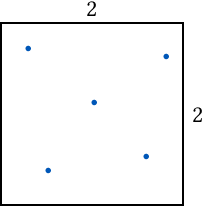
\includegraphics[width=\linewidth]{Images/image-2.png}}
\begin{proof}
    Divide square into 4 smaller squares. We now have 4 pigeonholes and 5 dots:
    \begin{figure}[H]
        \centering
        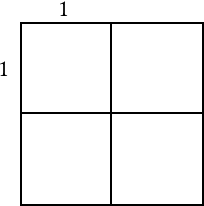
\includegraphics[width=100pt]{Images/image-3.png}
    \end{figure}
    These two points in the same pigeonhole have distance $\leq \sqrt{1^2+1^2}=\sqrt{2}$.
\end{proof}

\eg There exists two people in NYC who have exactly the same number of hairs on their head.

\eg There are 30 people at a party talking with each other. Afterwards, there will be two people who talked with the same number of people.
\begin{proof}
    If we put a person who talked to $i$ people into box $i$, we get 30 boxes; however, we cannot have someone who talked to 0 people and someone who talked at 29 people at the same time! Hence, we combine the box 0 and box 29, and only one of which could be the case.

    Now we have 29 boxes and 30 people. By pigeonhole principle, there must be two people who talked with the same amount of people.
\end{proof}

\begin{theorem}[Strong Pigeonhole Principle]
    Given pigeonholes $1,2,\dots,n$ with \uline{capacities} $c_1,c_2,\dots, c_n$ where $c_i\geq 0$; if we have at least $c_1+c_2+\dots+c_n+1$ pigeons in these pigeonholes, then at least one pigeonhole overflows.
\end{theorem}
\begin{proof}
    Suppose BWOC that no pigeonhole overflows. Then for all $i=1,2,\dots,n$, we have the number of pigeons in $i\leq c_i$.

    We add up and get inequalities:\begin{align*}
        \text{total \# pigeons} \leq c_1+c_2+\dots + c_n
    \end{align*}
    Contradiction!
\end{proof}

\eg There are five people supporting two teams. Then at least one team is supported by 3 people.
\begin{proof}
    Assume BWOC that the two teams only have two supporters. Let $c_1=c_2=2$. However, by SPP, $5\geq 2+2+1$, hence one pigeonhole overflows. Therefore, one team must have $>2$ supporters.
\end{proof}

\subsection{B2 First Ramsey Theorem}

There are 6 people taking a class. Then: \begin{itemize}[align=left]
        \item[\underline{either}] there exists 3 people such that each pair of them have previously taken a class together,
        \item[\underline{or (inclusive)}] there exists 3 people such that no two have taken a class together.
    \end{itemize}

\begin{theorem}
    If we have 6 vertices and we draw all edges between them (a $K_6$ graph)\sidenote{$K_6$ stands for \textit{complete graph on 6 vertices.} It has 15 edges.}, then for every possible way of coloring the edges \rt{red} and \bt{blue}, there must exist a \textbf{monochromatic} triangle.

    \[\begin{tikzcd}[ampersand replacement=\&,cramped]
        \& \bullet \\
        \bullet \&\& \bullet \\
        \bullet \&\& \bullet \\
        \& \bullet
        \arrow[color=magenta, no head, from=1-2, to=2-1]
        \arrow[color=magenta, no head, from=1-2, to=2-3]
        \arrow[color=magenta, no head, from=2-3, to=3-3]
        \arrow[color=cyan, no head, from=3-3, to=4-2]
        \arrow[color=magenta, no head, from=4-2, to=3-1]
        \arrow[color=cyan, no head, from=2-1, to=2-3]
        \arrow[color=magenta, no head, from=2-3, to=3-1]
        \arrow[color=cyan, no head, from=3-1, to=2-1]
        \arrow[color=magenta, no head, from=2-1, to=3-3]
        \arrow[color=cyan, no head, from=3-3, to=3-1]
        \arrow[color=magenta, no head, from=1-2, to=4-2]
        \arrow[color=magenta, no head, from=2-1, to=4-2]
        \arrow[color=cyan, no head, from=4-2, to=2-3]
        \arrow[color=cyan, no head, from=1-2, to=3-3]
        \arrow[color=cyan, no head, from=1-2, to=3-1]
    \end{tikzcd}\]
\end{theorem}
\begin{proof}
    \hypertarget{k6k3k3}{Pick} any vertex and call it $A$. It has 5 edges colored \rt{red} and \bt{blue}. By the SPP, there exists at least 3 edges of the same color. WLOG let these three edges be \rt{red} and call the other three vertices $B,C,D$.
    \[\begin{tikzcd}[ampersand replacement=\&,cramped]
        \&\& {\bullet B} \\
        {A\,\bullet} \&\&\& {\bullet C} \\
        \&\& {\bullet D}
        \arrow[color=magenta, no head, from=2-1, to=1-3]
        \arrow[color=magenta, no head, from=2-1, to=2-4]
        \arrow[color=magenta, no head, from=2-1, to=3-3]
        \arrow[dashed, no head, from=1-3, to=2-4]
        \arrow[dashed, no head, from=3-3, to=2-4]
        \arrow[dashed, no head, from=1-3, to=3-3]
    \end{tikzcd}\]
    \begin{itemize}
        \item If $BC$ is \rt{red}, then $ABC$ is a \rt{red} triangle.
        \item If $CD$ is \rt{red}, then $ACD$ is a \rt{red} triangle.
        \item If $BD$ is \rt{red}, then $ABD$ is a \rt{red} triangle.
        \item If none of the above has happened, then $BC,CD,BD$ are all \bt{blue}, meaning that $BCD$ is a \bt{blue} triangle!
    \end{itemize}
\end{proof}

\begin{theorem}
    If there are 5 instead of 6 vertices, then the above coloring prediction cannot be made with certainty.
\end{theorem}
\begin{proof}[Counterexample]
    \[\begin{tikzcd}[ampersand replacement=\&,cramped,column sep=tiny]
        \&\& \bullet \\
        \bullet \&\&\&\& \bullet \\
        \& \bullet \&\& \bullet
        \arrow[color=magenta, no head, from=1-3, to=2-1]
        \arrow[color=cyan, no head, from=2-1, to=2-5]
        \arrow[color=magenta, no head, from=1-3, to=2-5]
        \arrow[color=cyan, no head, from=1-3, to=3-2]
        \arrow[color=cyan, no head, from=1-3, to=3-4]
        \arrow[color=magenta, no head, from=2-1, to=3-2]
        \arrow[color=magenta, no head, from=3-2, to=3-4]
        \arrow[color=magenta, no head, from=3-4, to=2-5]
        \arrow[color=cyan, no head, from=3-2, to=2-5]
        \arrow[color=cyan, no head, from=2-1, to=3-4]
    \end{tikzcd}\]
\end{proof}


\subsection{B3 $K_p\to K_q,\, K_r$}

In graphy theory, $K_n$ is the \textbf{complete} graph on $n$ vertices.
\begin{table}[H]
    \centering
    \begin{tabular}{lcll}
        $K_1$ &$\bullet$& 1 vertex & 0 edges\\
        $K_2$ &\begin{tikzcd}[ampersand replacement=\&,cramped]
            \bullet \& \bullet
            \arrow[no head, from=1-1, to=1-2]
        \end{tikzcd}& 2 vertices & 1 edge\\[0.1in]
        $K_3$ &\begin{tikzcd}[ampersand replacement=\&,cramped,column sep=3pt,row sep=scriptsize]
            \& \bullet \\
            \bullet \&\& \bullet
            \arrow[no head, from=1-2, to=2-1]
            \arrow[no head, from=1-2, to=2-3]
            \arrow[no head, from=2-1, to=2-3]
        \end{tikzcd}& 3 vertices & 3 edges\\[0.3in]
        $K_4$ &\begin{tikzcd}[ampersand replacement=\&,cramped,sep=scriptsize]
            \bullet \& \bullet \\
            \bullet \& \bullet
            \arrow[no head, from=1-1, to=1-2]
            \arrow[no head, from=1-1, to=2-1]
            \arrow[no head, from=2-1, to=2-2]
            \arrow[no head, from=1-2, to=2-2]
            \arrow[no head, from=2-1, to=1-2]
            \arrow[no head, from=1-1, to=2-2]
        \end{tikzcd}& 4 vertices & 6 edges\\[0.3in]
        $K_5$ &\begin{tikzcd}[ampersand replacement=\&,cramped,column sep=1.5pt, row sep=13pt]
            \&\& \bullet \\
            \bullet \&\&\&\& \bullet \\
            \& \bullet \&\& \bullet
            \arrow[color=magenta, no head, from=1-3, to=2-1]
            \arrow[color=cyan, no head, from=2-1, to=2-5]
            \arrow[color=magenta, no head, from=1-3, to=2-5]
            \arrow[color=cyan, no head, from=1-3, to=3-2]
            \arrow[color=cyan, no head, from=1-3, to=3-4]
            \arrow[color=magenta, no head, from=2-1, to=3-2]
            \arrow[color=magenta, no head, from=3-2, to=3-4]
            \arrow[color=magenta, no head, from=3-4, to=2-5]
            \arrow[color=cyan, no head, from=3-2, to=2-5]
            \arrow[color=cyan, no head, from=2-1, to=3-4]
        \end{tikzcd}& 5 vertices & 10 edges\\[0.4in]
        $K_6$ &\begin{tikzcd}[ampersand replacement=\&,cramped,column sep=12pt, row sep=8pt]
            \& \bullet \\
            \bullet \&\& \bullet \\
            \bullet \&\& \bullet \\
            \& \bullet
            \arrow[color=magenta, no head, from=1-2, to=2-1]
            \arrow[color=magenta, no head, from=1-2, to=2-3]
            \arrow[color=magenta, no head, from=2-3, to=3-3]
            \arrow[color=cyan, no head, from=3-3, to=4-2]
            \arrow[color=magenta, no head, from=4-2, to=3-1]
            \arrow[color=cyan, no head, from=2-1, to=2-3]
            \arrow[color=magenta, no head, from=2-3, to=3-1]
            \arrow[color=cyan, no head, from=3-1, to=2-1]
            \arrow[color=magenta, no head, from=2-1, to=3-3]
            \arrow[color=cyan, no head, from=3-3, to=3-1]
            \arrow[color=magenta, no head, from=1-2, to=4-2]
            \arrow[color=magenta, no head, from=2-1, to=4-2]
            \arrow[color=cyan, no head, from=4-2, to=2-3]
            \arrow[color=cyan, no head, from=1-2, to=3-3]
            \arrow[color=cyan, no head, from=1-2, to=3-1]
        \end{tikzcd}& 6 vertices & 15 edges\\
    \end{tabular}
\end{table}
\rmk Note that $K_n$ has $1+2+3+\dots+(n-1)=\frac{n(n-1)}{2}$ edges, hence is the $n-1$-th triangular number.

Ramsey Theory uses the following language convention: the expression \begin{align*}
    K_p\to K_q,\, K_r
\end{align*}
represents a statement with the following meaning:

\defn If the edges of $K_p$ are colored \rt{red}/\bt{blue}, then it necessarily follows that either the $K_p$ contains a \rt{red $K_q$}, or $K_p$ contains a \bt{blue $K_r$} (or possibly both).

We want to know whether this statement is true for a given triple of $(p,q,r)$.

\eg We proved in  \hyperlink{k6k3k3}{\textbf{B2}} that $K_6\to K_3, K_3$.

\noneg We also showed that $K_5\to K_3,K_3$ is false \sidenote{write $K_5\not\to K_3,K_3$}by exhibiting a coloring of $K_5$ that does not have a red or blue triangle (counterexample).

\eg It is known that $K_{18}\to K_4, K_4$ and $K_{17}\not \to K_4,K_4$.

\eg Also, $K_9\to K_3,K_4$ and $K_8\not \to K_3,K_4$.\sidenote{Here we have to decide in advance which color goes with the $K_3$ and which goes with the $K_4$ due to asymmetry.}
\[\begin{tikzcd}[ampersand replacement=\&,cramped,row sep=26pt]
	\& \bullet \& \bullet \\
	\bullet \&\&\& \bullet \\
	\bullet \&\&\& \bullet \\
	\& \bullet \& \bullet
	\arrow[color=magenta, no head, from=1-2, to=2-1]
	\arrow[color=magenta, no head, from=1-3, to=1-2]
	\arrow[color=magenta, no head, from=2-4, to=1-3]
	\arrow[color=magenta, no head, from=3-4, to=2-4]
	\arrow[color=magenta, no head, from=4-3, to=3-4]
	\arrow[color=magenta, no head, from=4-2, to=4-3]
	\arrow[color=magenta, no head, from=3-1, to=4-2]
	\arrow[color=magenta, no head, from=2-1, to=3-1]
	\arrow[color=cyan, no head, from=2-4, to=1-2]
	\arrow[color=cyan, no head, from=3-4, to=1-2]
	\arrow[color=magenta, no head, from=4-3, to=1-2]
	\arrow[color=cyan, no head, from=4-2, to=1-2]
	\arrow[color=cyan, no head, from=3-1, to=1-2]
	\arrow[color=cyan, no head, from=2-1, to=1-3]
	\arrow[color=cyan, no head, from=3-1, to=1-3]
	\arrow[color=magenta, no head, from=4-2, to=1-3]
	\arrow[color=cyan, no head, from=4-3, to=1-3]
	\arrow[color=cyan, no head, from=3-4, to=1-3]
	\arrow[color=cyan, no head, from=2-1, to=2-4]
	\arrow[color=magenta, no head, from=3-1, to=2-4]
	\arrow[color=cyan, no head, from=4-2, to=2-4]
	\arrow[color=cyan, no head, from=4-3, to=2-4]
	\arrow[color=magenta, no head, from=2-1, to=3-4]
	\arrow[color=cyan, no head, from=3-1, to=3-4]
	\arrow[color=cyan, no head, from=4-2, to=3-4]
	\arrow[color=cyan, no head, from=3-1, to=4-3]
	\arrow[color=cyan, no head, from=2-1, to=4-3]
\end{tikzcd}
\]
\[\text{This $K_8$ has no red triangle and no blue }K_4.\]

\addlink{Ramsey's theorem}
\theorem[Ramsey] Let $q,r$ be positive integers. Then there always exists a positive integer $p$ such that \[K_p\to K_q,K_r\] is true.

We would see the following tabel giving us values of $p$ that work.

Define a function $N(q,r)$ recursively: \sidenote{$q,r\in \Z^+$}
\begin{itemize}
    \item Base case: $N(1,r)=N(q,1)=1$
    \item Recurrence: $N(q,r)=N(q-1,r)+N(q,r-1)$ if $q,r\geq 2$.
\end{itemize}
\hypertarget{tableforN}{}
We compute the value of $N(q,r)$ for:\sidenote{They do look like simplex numbers!}
\begin{table}[H]
    \centering
    \begin{tabular}{lcccccc}
    $q\backslash r$ & 1 & 2 & 3  & 4  & 5   & 6   \\
    1                  & 1 & 1 & 1  & 1  & 1   & 1   \\
    2                  & 1 & 2 & 3  & 4  & 5   & 6   \\
    3                  & 1 & 3 & 6  & 10 & 15  & 21  \\
    4                  & 1 & 4 & 10 & 20 & 35  & 56  \\
    5                  & 1 & 5 & 15 & 35 & 70  & 126 \\
    6                  & 1 & 6 & 21 & 56 & 126 & 252
    \end{tabular}
\end{table}
We would want to prove that $K_{N(q,r)}\to K_q,K_r$ for all $q,r\geq 1$.
\begin{proof}
    By induction.
    \begin{enumerate}[align=left]
        \item[\textit{Base case}:] \begin{tabular}[t]{rl}
            If $q=r=1$, then $N=1$, we need to show that& $K_1\to K_1,K-r$\\
            and & $K_1\to K_q,K_1$
        \end{tabular} for all $q,r$. 
        
        That is, suppose $K_1$ has its edges colored \rt{red}/\bt{blue}, then there exists a \rt{red $K_1$} or a \bt{blue $K_r$}, and \textit{vice versa}. 
        
        Since there are no edges, this is vacuously true.

        \item[\textit{Inductive step}:] \hypertarget{ramseyInductive}{We} will show\sidenote{This works because as we fill out the table above, each new number we write in will work because it's the sum of the left and above numbers and they both work.} 
        that \uline{if we are given that} $A,B$ are numbers such that \begin{align*}
            K_A&\to K_{q-1},K_r\\
            \text{and }K_B&\to K_q, K_{r-1}
        \end{align*}
        are true, \uline{then} $K_{A+B}\to K_q,K_r$.

        Consider $K_{A+B}$ colored \rt{red} and \bt{blue}. We will show that it has a \rt{red $K_q$} or a \bt{blue $K_r$}.
        
        Pick a vertex and call it $X$. It would have $A+B-1$ edges in total. We claim that \dashuline{$X$ either has at least $A$ \rt{red} edges, or at least $B$ \bt{blue} edges}. This is indeed true, because if not, the number of \rt{red} edges would be $\leq A-1$ and the number of \bt{blue} edges would be $\leq B-1$ and so the total number of edges would be $\leq A+B-2<A+B-1$, which is a contradiction.

        Now, if $X$ has a \rt{red claw} of size $A$:\sidenote{The neighbouring vertices connected by black edges form $K_A$, yet to be colored.}
        \[\begin{tikzcd}[ampersand replacement=\&,cramped]
            X \&\& \dots \& {K_A} \\
            \&\& \bullet \\
            \dots \& \bullet
            \arrow[color=magenta, dashed, no head, from=1-1, to=1-3]
            \arrow[color=magenta, no head, from=1-1, to=2-3]
            \arrow[color=magenta, no head, from=1-1, to=3-2]
            \arrow[color=magenta, dashed, no head, from=1-1, to=3-1]
            \arrow[no head, from=1-3, to=2-3]
            \arrow[no head, from=1-3, to=3-2]
            \arrow[no head, from=2-3, to=3-2]
            \arrow[no head, from=3-1, to=3-2]
            \arrow[no head, from=3-1, to=2-3]
        \end{tikzcd}\]
        From our inductive hypothesis $K_A\to K_{q-1},K_r$, we must have \begin{itemize}[align=left]
            \item[\textbf{either}] \rt{red $K_{q-1}$}, in which case we combine with the vertex $X$ and the red claw to get at least one \rt{red $K_q$}.
            \item[\textbf{or}] \bt{blue $K_r$}, in which case we are done. 
        \end{itemize}
        Similarly, if $X$ has a \bt{blue claw} of size $B$, then we make the same argument.
        \vspace{0.2in}
        
        Hence, we know that $K_{A+B}\to K_q,K_r$ is true whenever $K_A\to K_{q-1},K_r$ and $K_B\to K_{q},K_{r-1}$.
    \end{enumerate}
\end{proof}

\subsection{B4 Ramsey numbers}
Recall: Let $m,n$ be positive integers. We know that there are numbers $p\in \N$ such that $K_p\to K_m,K_n$.

\rmk If $p$ works, then so does any $q\geq p$ as $K_q$ would contain copies of $K_p$.

So the question becomes, if we have $K_p\to K_m,K_n$, is $p$ the \textbf{smallest} such number?

\defn The \textbf{Ramsey number} $r(m,n)$ is the smallest such number.

\eg We know $K_6\to K_3,K_3$ but $K_5\not\to K_3,K_3$, so $r(3,3)=6$.

\eg Mathematicians have proved that \begin{align*}
    K_{48} &\to K_5,K_5\\
    K_{42} &\not\to K_5,K_5
\end{align*}
so we have $43\leq r(5,5)\leq 48$.

\rmk In general, \begin{align*}
    K_N&\to K_m, K_n \iff r(m,n)\leq N\\
    K_{N-1} &\not\to K_m,K_n \iff r(m,n)\geq N
\end{align*}
Need both to get the precise value of $r(m,n)$.

\begin{proposition} Properties of Ramsey numbers:
\begin{enumerate}[label=(\alph*)]
    \item $r(3,3)=6$ \sidenote{proven in  \hyperlink{k6k3k3}{\textbf{B2}}}
    \item $r(m,n) = r(n,m)$\sidenote{symmetry}
    \item $r(1,n)=1$\sidenote{$K_1\to K_1,K_n$, $K_0\not\to K_1,K_n$}
    \item $r(2,n)=n$
    \item $r(m,n)\leq r(m-1,n)+r(m,n-1)$ for all $m,n\geq2$
\end{enumerate}
\begin{proof}[Proof for (d)]
    Claim: $K_2\to K_2,K_n$, $K_{n-1}\not\to K_2,K_n$.
    
    Color $K_n$. If all edges are blue then we have a \bt{blue $K_n$}. Else we have some red edges, so we have some \rt{red $K_2$}.

    Now color $K_{n-1}$ all blue: we realize that we don't have any red $K_2$, but we don't have a blue $K_n$ either!
\end{proof}
\begin{proof}[Proof for (e)]
    Let $A=r(m-1,n)$, $B=r(m,n-1)$. We have shown that if $K_A\to K_{m-1},K_n$ and $K_B\to K_{m},K_{n-1}$, then $K_{A+B}\to K_m, K_n$. Hence $r(m,n)\leq A+B$.
\end{proof}
\end{proposition}

Known facts:
\begin{align*}
    r(2,2) &=2\\
    r(3,3) &=6\\
    r(4,4) &=18\\
    43\leq r(5,5)&\leq 48\\
    102\leq r(6,6)&\leq 165
\end{align*}

\subsection{B5 A lower bound for $r(m,n)$}
Our \hyperlink{tableforN}{table of $N(m,n)$} gave us upper bonds for $r(m,n)$. Specifically, \begin{align*}
    r(m,n)\leq N(m,n)=\frac{(n+m-2)!}{(n-1)!(m-1)!}=
   {{m+n-2}\choose{m-1}}
\end{align*}

What about lower bound?

\begin{theorem}
    \begin{align*}
        r(m,n)\geq (m-1)(n-1)+1
    \end{align*}
    \ifnif $K_{(m-1)(n-1)}\not\to K_m, K_n$
\end{theorem}

\begin{proof}
    We prove this by exhibiting a coloring of $K_{(m-1)(n-1)}$ that has no red $K_m$, no blue $K_n$.
    
    Place vertices in grid:
    \[\begin{tikzcd}[ampersand replacement=\&,cramped,sep=small]
        \bullet \& \bullet \& \dots \& \bullet \\
        \bullet \& \bullet \& \dots \& \bullet \\
        \vdots \& \vdots \& \ddots \& \vdots \\
        \bullet \& \bullet \& \dots \& \bullet
        \arrow["{m-1\text{ rows}}"', shift right=4, draw=none, from=1-1, to=4-1]
        \arrow["{n-1\text{ columns}}"', shift right=5, draw=none, from=4-1, to=4-4]
    \end{tikzcd}\]
    Coloring rule of edges: If two vertices are in the same row, color the edges \bt{blue}. If two vertices are in the same column, color the edges \rt{red}. Every other edge arbitrary.

    Claim: there exists no \rt{red} $K_m$.

    Consider the $m$ vertices of such a $K_m$. There are $m-1$ rows. Pigeonhole principle ensures that some vertices must be in the same row. But that edge must be \bt{blue}! So this is not a red $K_m$. Similarly, there are no blue $K_n$.
\end{proof}

Thus, we get: $\displaystyle (m-1)(n-1)+1\leq r(m,n)\leq \frac{(n+m-2)!}{(n-1)!(m-1)!}=
{{m+n-2}\choose{m-1}}$.

Observe there is still a huge gap between the bounds. Could we get better?

\subsection{B6 The ``parity'' improvement}
Our methods have shown that $K_{10}\to K_3,K_4$. But it is actually true that $K_{9}\to K_3,K_4$. Why?
\begin{proof}
    Given $K_9$ colored red or blue. We seek a \rt{red $K_3$} or a \bt{blue $K_4$}. 
    
    That is to say that if we ever see a \rt{red 4-claw}, then we are done!\sidenote{See \hyperlink{k6k3k3}{this} argument.}
    \[\begin{tikzcd}[ampersand replacement=\&,cramped]
        \bullet \&\& \bullet \\
        \&\& \bullet \\
        \& \bullet \& \bullet
        \arrow[color=magenta, no head, from=1-1, to=1-3]
        \arrow[color=magenta, no head, from=1-1, to=3-3]
        \arrow[color=magenta, no head, from=1-1, to=2-3]
        \arrow[color=magenta, no head, from=1-1, to=3-2]
    \end{tikzcd}\]

    In addition, if we ever see a \bt{blue 6-claw}, then we are also done because $K_6\to K_3,K_3$ and we either have a \rt{red $K_3$} or a \bt{blue $K_3$}, which would have to combine with the other vertex to get a blue $K_4$.

    Now suppose we neither have a red 4-claw nor a blue 6-claw. This implies that each vertex has $\leq 3$ \rt{red} edges, and $\leq 5$ blue edges. However, in a $K_9$, \dashuline{each vertex only has 8 edges}, so they must \dashuline{exactly each have 3 red edges and 5 blue edges}. Does this exist? We realize that to make this happen, we have:\begin{itemize}
        \item 9 vertices
        \item Each vertex has 3 red edges
        \item Every edge belongs to two vertices
    \end{itemize}
    Hence, we need to have exactly $\frac{3\times9}{2}=13.5$ red edges, but this cannot happen because we need a whole number of edges! Thus, it is not possible that we neither have a red 4-claw nor a blue 6-claw.
\end{proof}

\begin{lemma}[Ramsey inductive step improved by parity]
    Suppose\sidenote{Also seen \hyperlink{ramseyInductive}{here}.} \begin{align*}
        K_A&\to K_{q-1},K_r\\
        \text{and }K_B&\to K_q, K_{r-1}
    \end{align*}
    are true, \uline{then} $K_{A+B}\to K_q,K_r$.

    In addition, if $A,B$ are \textbf{both even numbers}, then $K_{A+B-1}\to K_q,K_r$.
\end{lemma}

\subsection{B7 Variations}
\subsubsection{\rt{More }\gt{colors}\bt{!} }

For example:\begin{align*}
    K_p\to K_a,K_b,K_c
\end{align*}
(given $K_p$ colored \rt{red}, \bt{blue}, \gt{green}, it must contain a red $K_a$, or a blue $K_b$, or a green $K_c$.)

\eg It is known that $K_{17}\to K_3,K_3,K_3$.
\begin{proof}[Proof sketch]
    Pick a vertex which has 16 edges. We observe $16\div 3=5\frac{1}{3} \implies $ at least one color occurs 6 times (i.e. we can see a red/blue/green 6-claws).
\end{proof}

\rmk $r(a,b,c)$ is the smallest number that works for the above.

\subsubsection{Other graphs}
\begin{itemize}[align=left]
    \item[Paths: ] \[\begin{tikzcd}[ampersand replacement=\&,cramped,sep=small]
        {P_1} \& \bullet \\
        {P_2} \& \bullet \& \bullet \\
        {P_3} \& \bullet \& \bullet \& \bullet \\
        {P_4} \& \bullet \& \bullet \& \bullet \& \bullet
        \arrow[no head, from=2-2, to=2-3]
        \arrow[no head, from=3-2, to=3-3]
        \arrow[no head, from=3-3, to=3-4]
        \arrow[no head, from=4-2, to=4-3]
        \arrow[no head, from=4-3, to=4-4]
        \arrow[no head, from=4-4, to=4-5]
    \end{tikzcd}\]
    \item[Claws: ]  \[\begin{tikzcd}[ampersand replacement=\&,cramped,column sep=small,row sep=tiny]
        {K_{1,1}} \& \bullet \& \bullet \& {K_{1,4}} \& \bullet \& \bullet \\
        {K_{1,2}} \& \bullet \& \bullet \&\&\& \bullet \\
        \&\& \bullet \&\&\& \bullet \\
        {K_{1,3}} \& \bullet \& \bullet \&\&\& \bullet \\
        \&\& \bullet \\
        \&\& \bullet
        \arrow[no head, from=1-2, to=1-3]
        \arrow[no head, from=2-2, to=2-3]
        \arrow[no head, from=2-2, to=3-3]
        \arrow[no head, from=4-2, to=4-3]
        \arrow[no head, from=5-3, to=4-2]
        \arrow[no head, from=6-3, to=4-2]
        \arrow[no head, from=1-5, to=1-6]
        \arrow[no head, from=2-6, to=1-5]
        \arrow[no head, from=3-6, to=1-5]
        \arrow[no head, from=4-6, to=1-5]
    \end{tikzcd}\]
\end{itemize}

\eg Show that $r(K_{1,3}, K_{1,3}) = 6$.
\begin{proof}
    We know $K_6\to K_3,K_3$. Pick a vertex that has 5 neighbors. By the strong pigeonhole principle, we must have three edges of the same color $\implies$ either red or blue $K_{1,3}$.
\end{proof}

\section{C Counting}
\subsection{C1 Three principles}
\subsubsection{Addition principle}\sidenote{aka. counting by cases}
\defn If a set $S$ is \textit{partitioned}\sidenote{that is, $S=\bigcup S_i$ and $S_i\cap S_j=\emptyset$ whenever $i\neq j$} into subsets $S_1,S_2,\dots S_n$, then the cardinality of $S$ is $$|S|=|S_1|+\dots +|S_n|.$$

The art lies in:\begin{itemize}
    \item making each $S_i$ easy to count, and
    \item not having too many $S_i$ if there is no formula for $|S_i|$.
\end{itemize}

\rmk[Variations] If the $S_i$ cover $S$ but they overlap\sidenote{The inclusion/exclusion principle handles overlaps precisely}, then we have the inequality $\displaystyle |S|<\sum_{i=1}^{n}|S_i|$ because the overlap implies that we are \textit{overcounting}.

\eg Let $S$ be the set of \textit{good}\sidenote{\textit{good} meaning no adjacent elements} subsets of $[5]=\{1,2,3,4,5\}$. We could first try:\begin{itemize}
    \item $S_1$ contains the subsets that contain 5
    \item $S_2$ contains the subsets that don't contain 5
\end{itemize}
We have previously shown that $|S_1|=$ number of \textit{good} subsets of [3] and $|S_2|=$ number of \textit{good} subsets of [4].

Alternatively, we could also let $T_i$ be the \textit{good} subsets of $[5]$ with cardinality $i$. Then $S$ is \uline{partitioned} into $T_0\cup T_1\cup T_2\cup T_3$. We count:
\[\begin{tikzcd}[ampersand replacement=\&,cramped]
	{T_0:} \& \emptyset \& {|T_0|=1} \\
	{T_1:} \& {1,2,3,4,5} \& {|T_1|=5} \\
	{T_2:} \& {13,14,15,24,25,35} \& {|T_2|=6} \\
	{T_3:} \& 135 \& {|T_3|=1}
	\arrow["{|S|=13}", shift left=5, bend left=40, no head, from=1-3, to=4-3]
\end{tikzcd}\]

\subsubsection{Subtraction principle}
\defn Let $A\subseteq S$ and $A^c$ be its complement in $S$. Then $A, A^c$ partition $S$ and $|S|=|A|+|A^c|$. This means that $$|A|=|S|-|A^c|.$$

\eg How many 2-digit numbers have distinct nonzero digits?

Let $S$ be the set of all 2-digit numbers $\{10,11,\dots,99\}$ and let $A$ be the subset of those with nonzero distinct digits. We count:\begin{align*}
    A^c: &11,22,\dots,99 &&\text{(distinct fails)}\\
    &10,20,\dots, 90 &&\text{(nonzero fails)}
\end{align*}
Hence $|A|=|S|-|A^c|=90-18=72$.

\subsubsection{Multiplication principle}
\defn Suppose we have to do two tasks in sequence\sidenote{Note: sometimes the 2nd task could depend on the 1st one}. We suppose:\begin{itemize}
    \item Task 1 has $m$ outcomes
    \item Task 2 has $n$ outcomes, regardless of how Task 1 was carried out.
\end{itemize}
Then there are $mn$ ways of carrying out both tasks.\sidenote{Similarly for 3 or more tasks in sequence}

\eg How many 2-digit numbers have distinct nonzero digits?

Let \circled{a}\circled{b} be the two digits in these numbers. Let Task 1 be selecting digit \circled{a} and Task 2 be selecting digit \circled{b}.\begin{itemize}
    \item Task 1: 9 ways (1,2,\dots,9)
    \item Task 2: 8 ways (1,2\dots,9 but not same as \circled{a})
\end{itemize}
Hence there are $9\times 8=72$ such numbers.

\cautiouseg How many \textbf{odd} numbers in the range 1000-9999 have distinct digits?
\begin{itemize}[align=left]
    \item[\textbf{Attempt 1}:] Let \circled{a}\circled{b}\circled{c}\circled{d} be the 4 digits in these numbers and assign them Tasks 1-4. We have: \begin{itemize}
        \item Task 1: 9 ways (1-9)
        \item Task 2: 9 ways (0-9 except \circled{a})
        \item Task 3: 8 ways (0-9 except \circled{a},\circled{b})
        \item \rt{Task 4}: Could be 2 or 3 or 4 or 5 (depending on how many odd digits had already been used)
    \end{itemize}
    Hence, the best we can say\sidenote{BAD! This is a large range!} here is that the answer is between $9\times9\times8\times2$ and $9\times9\times8\times5$.

    \item[\textbf{Attempt 2}:] Let \circled{a}\circled{b}\circled{c}\circled{d} be the 4 digits in these numbers and try the order \circled{d}\circled{a}\circled{b}\circled{c} for Tasks 1-4. We have: \begin{itemize}
        \item Task 1: 5 ways $(1,3,5,7,9)$
        \item Task 2: 8 ways (1-9 except \circled{d})
        \item Task 3: 8 ways (0-9 except \circled{a}, \circled{d})
        \item Task 4: 7 ways (0-9 except \circled{a}, \circled{d}, \circled{b})
    \end{itemize}
    Therefore, the number of ways is $5\times 8\times 8\times 7=2240$.
\end{itemize}

\eg How many numebrs $0,1,\dots 99999$ have exactly one digit 6?

We can assign tasks:\begin{itemize}
    \item Task 1: choose a location for 6, giving us 5 ways
    \item Task 2: assign the remaining digits from left to right, giving us $9^4$ ways
\end{itemize}

Hence there are $5\times 9^4=32805$ such numbers.

\noneg How many integers $0,1,\dots 99999$ have \textit{at least} one digit 6?

\textbf{Attempt:} We can assign tasks:\begin{itemize}
    \item Task 1: choose a location for 6, giving us 5 ways
    \item Task 2: assign the remaining digits from left to right, giving us $10^4$ ways
\end{itemize}

But the answer of 50000 is \rt{\textbf{wrong}}! But why?

The counting process for this problem is corresponding the ways of performing tasks to valid 5-digit numbers:
\drawing{0.6\linewidth}{image-4.png}
We have correctly counting the \gt{green} set. However, for this to count the \bt{blue} set, we need $f$ to be \textbf{bijective}. That is, every valid number must be obtained in exactly one way. However, in this case, our $f$ is surjective but not injective. For instance, 62516 will be counted \textit{twice}:\begin{itemize}
    \item 6\_\_\_\_ then 62516; or
    \item \_\_\_\_6 then 62516.
\end{itemize}
Hence, 50000 > correct answer!

\textbf{Correct way:} Using the subtract principle to deduct numbers that don't have 6: $10^5-9^5=40951<50000$.

\subsection{C2 Probability}
\defn \begin{align*}
    \text{Probability} = \frac{\text{number of favourable cases}}{\text{number of total cases}}
\end{align*}

\eg Probability of 3 dice rolling the same number: $P=\frac{6}{6^3}=\frac{1}{36}$.

\subsection{C3 The counting framework}
Here is a very general problem:

``How many distinguishable ways to map a multiset $S$ to a multiset $T$ satisfying given constraints?''

\eg There are fruits and plates. Let $S=\{3\cdot \text{apple}, 1\cdot \text{banana}\}$ and $T=\{2\cdot \text{circle}, 1\cdot \text{rectangle}\}$. How many ways are there to serve fruit on plates such that the rectangular plate has an even number of fruit?
\drawing{0.6\linewidth}{image-5.png}

\textbf{Ans:} Organize by number of fruit on rectangle.
\drawing{0.6\linewidth}{image-6.png}
\drawing{0.6\linewidth}{image-7.png}
\drawing{0.6\linewidth}{image-8.png}

Hence there are 9 ways.

\subsubsection{The general counting problem}
Let there be multisets \begin{align*}
    S&=\{a_1\cdot 1, a_2\cdot2, \dots, a_s\cdot s\} &\text{object types }1,2,\dots,s\\
    T&=\{b_1\cdot U_1, b_2\cdot U_2,\dots,b_t\cdot U_t\} &\text{box types }U_1,\dots,U_t\\
\end{align*}
How many distinguishable maps $f: S\to T$ are there, subject to restrictions on the numbers $u_i=\left|\inv{f}(U_i)\right|$?\sidenote{The number of items mapped to boxes of type $U_i$}

\rmk[Special cases] To recognize which situation applies to the problem:
\begin{itemize}
    \item By objects:\begin{itemize}
        \item Distinct: $S=\{1,2,\dots,s\}$
        \item Identical: $S=\{s\cdot 1\}$
    \end{itemize}
    \item By boxes: \begin{itemize}
        \item Distinct: $T=\{U_1,\dots, U_t\}$
        \item Identical: $T=\{t\cdot U_1\}$
    \end{itemize}
    \item For each case above, we can apply constraints:\begin{itemize}
        \item $0\leq u_i\leq 1$
        \item $0\leq u_i<\infty$\qquad{no constraint}
        \item $1\leq u_i<\infty$\qquad{nonempty}
        \item $0\leq u_i\leq n_i$ for some $n_i\in \N_0$\qquad{max. capacity}
        \item $u_i\in N_i\subseteq \N$
    \end{itemize}
\end{itemize}
\drawing{0.95\linewidth}{table3-1.pdf}

\eg We have 10 distinct books to be shared between 2 children. Each child needs 2 books to avoid a crisis.\sidenote{Table entry \circled{15}}
\begin{itemize}
    \item Distinct objects $\{1,2,\dots,10\}$
    \item Distinct boxes $\{U_1,U_2\}$
    \item Constraints: $u_i\in [2,\infty[$
\end{itemize}

\eg[Attempt 1] 10 distinct books, 5 of them to be arranged on shelf (order matters)\sidenote{Table entry \circled{15}}
\begin{itemize}
    \item $S=\{1,2,\dots,10\}$
    \item $T=\{U_1,U_2,\dots,U_5, \rt{U_6}\}$ (positions on shelf + extra for unshelved books)
    \item $u_1=\dots=u_5=1, u_6=5$
\end{itemize}

\eg[Attempt 2] 10 distinct books, 5 of them to be arranged on shelf (order matters)\sidenote{Table entry \circled{1}, easier!}
\begin{itemize}
    \item $S=\{1,2,\dots,5\}$ (numbered stickers to arrange books)
    \item $T=\{U_1,U_2,\dots,U_{10}\}$ (10 books)
    \item $0\leq u_1\leq 1$ (each book can get 0 or 1 sticker)
\end{itemize}

\eg I have 10 books and will take 5 on holiday.
\begin{itemize}
    \item Take 1:\sidenote{Table entry \circled{15}} \begin{itemize}
        \item $S=\{1,2,\dots,10\}$
        \item $T=\{U_1,U_2\}$
        \item $u_1=u_2=5$
    \end{itemize}
    \item Take 2:\sidenote{Table entry \circled{2}} \begin{itemize}
        \item $S=\{5\cdot 1\}$ (identical `stickers' marking on-holiday)
        \item $T=\{U_1,U_2\,\dots,U_{10}\}$
        \item $0\leq u_1\leq 1$ (each book can get 0 or 1 sticker)
    \end{itemize}
\end{itemize}

\subsection{C4 Permutations of a set}
\rmk Recall $[n]=\{1,2,\dots,n\}$.

\defn Let $0\leq s\leq t$. \begin{itemize}
    \item An \textbf{$s$-permutation} of $[t]$ is an ordered list of $s$ distinct elements of $[t]$.
    \item A \textbf{$t$-permutation} of $[t]$ is just a \textbf{permutation} of $[t]$.
\end{itemize}

\eg 10 books, arrange 5 on shelf: 5-perm of $[10]$
\eg 20 athletes, Gold, Silver and Bronze awarded: 3-perm of [20]

\begin{theorem}
    The number of $s$-perms of $[t]$ is \[\underset{s\text{ terms}}{\underbrace{t(t-1)\dots (t-s+1)}}\]
\end{theorem}
\begin{proof}
    Select elements of the list one-by-one. We have $t$ ways to pick the first, $t-1$ ways of picking the second, etc.
\end{proof}

\defn[$s$-th falling-factorial function] This inspires the following notation \[(x)_s=x(x-1)\dots(x-s+1)=\frac{t!}{(t-s)!}\]\sidenote{There is also a rising $(x)^s=x(x+1)\dots(x+s-1)$}
\rmk $(x)_0=1, (n)_n=n!$

\eg Number of ways to shelve 5 books out of 10 is $$(10)_5=10\times9\times8\times7\times6=30240$$

\subsection{C5 Circular permutations}

A circular 5-perm of $[n]$ is an arrangement of $s$ distinct elements of $[n]$ around a round table. The difference from a non-circular perm is that the orientation of the table does not matter! How many ways to do so?

If there is a head of the table and positions are marked clockwise, then it would be the same as the $s$-perm $(n)_s$.

However, we consider all ways of marking the `head' of the tablen to be equivalent, so we divide $s$ upon that. Hence, we get the answer $\displaystyle\frac{1}{s}(n)_s=\frac{n!}{s(n-s)!}$.

\subsection{C6 Table entries 3,4,5}
\begin{itemize}
    \item \circled{3}: $s$ distinct objects, $t$ identical boxes, 0 or 1 per box.
    \[\# \text{ ways} = \begin{cases}
        1 & s\leq t\\
        0 &\text{otherwise}
    \end{cases}\]
    \item \circled{4}: $s$ identical objects, $t$ identical boxes, 0 or 1 per box.
    \[\# \text{ ways} = \begin{cases}
        1 & s\leq t\\
        0 &\text{otherwise}
    \end{cases}\]
    \item \circled{5}: $s$ distinct objects, $t$ distinct boxes, no restrictions.
    \[\# \text{ ways} = \underset{s \text{ times}}{\underbrace{t\times t\times\dots \times t}}=t^s\]
\end{itemize}

\rmk $0^0=1$ in combinatorics.\sidenote{NOT in analysis!!}
\drawing{0.95\linewidth}{table3-1.pdf}

\subsection{C7 Combinations of sets: table entries 2,6,10}
If we let $0\leq s\leq t$, then an \textbf{$s$-combination of} [$t$] is a subset of size $s$ of $[t]$.

\defn The binomial coefficient $t\choose s$ is defined (combinatorially) to be the number of $s$-combinations of $[t]$.

\begin{theorem}
    \[{t\choose s} = \frac{(t)_s}{s!}=\frac{t!}{(t-s)!s!}\]
\end{theorem}
\begin{proof}
    Consider the number of $s$-perms of $[t]$. 
    
    We can count it directly: $(t)_s$.

    Alternatively, make task 1 `selecting a subset of size $s$', which gives us $t\choose s$ ways. Make task 2 the ways of ordering a subset, which give $s!$ ways. By multiplication principle, the number of $s$-perms of $[t]$ is ${t\choose s}s!$.

    We have $(t)_s={t\choose s}s!$, giving us the formula above.
\end{proof}


\eg All of the following are equivalent and satisfy table entry \circled 2\sidenote{$0\leq u_i\leq 1$}:
\begin{itemize}
    \item Select $s$ books out of $t$ distinct books;
    \item Place $s$ stickers on $t$ books, at most one sticker per book;
    \item Put $s$ identical objects into $t$ distinct boxes, each box can only have at most 1 object.
\end{itemize}

\eg These equivalent problems satisfy table entry \circled 6:\sidenote{$0\leq u_i<\infty$}
\begin{itemize}
    \item Solutions to $x_1+x_2+x_3+x_4+x_5=12$ where $x_i\geq 0$ are integers.
    \item Packing a box of 12 bagels of 5 different types of bagels with unlimited supply.
    \item Number of permutations of 12 objects and 4 `drawer dividers': \[\bullet\bullet \,|\, \bullet\bullet\bullet \,|\, \bullet\bullet\,|\, \bullet\bullet\bullet\bullet \,|\, \bullet\]
\end{itemize}

\rmk In general, when we count the number of anagrams $s~\bullet$s and $t-1 \mid$s, there are $s+t-1$ total symbols. We must select $s$ of the $s+t-1$ positions to be $\bullet$. Hence, the number of ways would be\sidenote{LHS is choose $\bullet$, RHS is choose $\mid$.} \[{{s+t-1}\choose s}={{s+t-1}\choose t-1}\]

\eg Entry \circled{10} is the same as \circled 6 except that each box must be nonempty:\begin{itemize}
    \item Solutions to $x_1+\dots + x_s=t$ where $x_i\geq 1$ integers.
    \item Select $s$ bagels from $t$ types, with each type chosen at least once. 
    
    This reduces to the prev problem: select one of each type of bagel first; then, we choose $s-t$ bagels of $t$ types.

    \item Anagrams with $s$ $\bullet$s and $t-1$ $\mid$: must avoid $||$ and $|$ at beginning or end. Then we could think about placing $t-1$ dividers in the $s-1$ spaces between $\bullet$s, giving us $s-1\choose t-1$ ways.
\end{itemize}

\subsection{C8 Anagrams}
\eg Find the number of anagrams of the word \begin{center}
    COMBINATORIALISTICALLY
\end{center}
First, suppose all 22 letters were distinct. We put subscripts:
\[\mathrm{C_1O_1MBI_1NA_1T_1O_2RI_2A_2L_1I_3ST_2I_4C_2A_3L_2L_3Y}\]
Now we have this multiset: \[\{\mathrm{2C, 2O, M, B, 4I, N, 3A, 2T, R, 3L, S, Y}\}\]
We want to find the ways of arranging this!
\begin{itemize}
    \item Assuming everything is distinct: 22! ways.
    \item Same assumption but with two tasks in multiplication:\begin{itemize}
        \item Task 1: Arrange without subscripts (what we want)
        \item Task 2: Add subscripts: the number of ways to add them is \[2!\times 2!\times 1!\times 1!\times 4!\times 1!\times 3!\times 2!\times 1!\times 3!\times 1!\times 1!\]
    \end{itemize}
\end{itemize}
\addlink{Multinomial coefficient}
Therefore, our answer would be (in multinomial coefficient)\sidenote{DO NOT LEAVE OUT 1s}\begin{align*}
    &\frac{22!}{2!\times 2!\times 1!\times 1!\times 4!\times 1!\times 3!\times 2!\times 1!\times 3!\times 1!\times 1!}
    =&{ 22\choose 2,2,1,1,4,1,3,2,1,3,1,1}
\end{align*}

\subsection{C9 More circular tables}
\eg \label[example]{alien-conference} An alien conference has 9 Martian hare delegates and 16 Jovian hare delegates, with each type of hare identical. How many distinguishable ways are there to seat them at a circular table?

Method: first consider the ways of arrangement at a marked table.
\[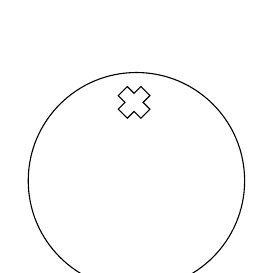
\begin{tikzpicture}[x=0.75pt,y=0.75pt,yscale=-1,xscale=1]
    %uncomment if require: \path (0,300); %set diagram left start at 0, and has height of 300
    
    %Shape: Circle [id:dp9867838680866461] 
    \draw   (77,85.13) .. controls (77,56.34) and (100.34,33) .. (129.13,33) .. controls (157.92,33) and (181.26,56.34) .. (181.26,85.13) .. controls (181.26,113.92) and (157.92,137.26) .. (129.13,137.26) .. controls (100.34,137.26) and (77,113.92) .. (77,85.13) -- cycle ;
    %Shape: Cross [id:dp053203375302823375] 
    \draw   (131.27,39.77) -- (135.62,44.13) -- (132.36,47.39) -- (135.62,50.66) -- (131.27,55.02) -- (128,51.75) -- (124.73,55.02) -- (120.38,50.66) -- (123.64,47.39) -- (120.38,44.13) -- (124.73,39.77) -- (128,43.04) -- cycle ;
    \end{tikzpicture}
    \]

\begin{itemize}
    \item We seat 9 Martian hares and fill out the rest with Jovian ones: $\displaystyle {25\choose 9}$.
    \item We place all hares (the answer we want) and then mark the table. In the end we should get the same answer of $\displaystyle{ 25\choose 9}$.\begin{itemize}
        \item How do we mark the table? There are 25 places that can be marked, but \dashuline{not all of them are distinct}! For instance:
        \[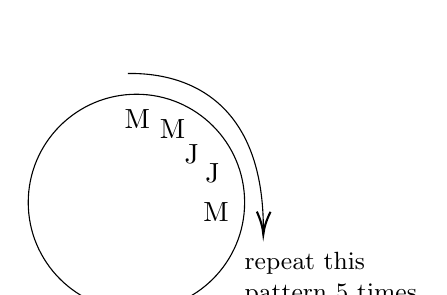
\begin{tikzpicture}[x=0.75pt,y=0.75pt,yscale=-1,xscale=1]
            %uncomment if require: \path (0,300); %set diagram left start at 0, and has height of 300
            
            %Shape: Circle [id:dp9867838680866461] 
            \draw   (77,85.13) .. controls (77,56.34) and (100.34,33) .. (129.13,33) .. controls (157.92,33) and (181.26,56.34) .. (181.26,85.13) .. controls (181.26,113.92) and (157.92,137.26) .. (129.13,137.26) .. controls (100.34,137.26) and (77,113.92) .. (77,85.13) -- cycle ;
            %Curve Lines [id:da9747269900319728] 
            \draw    (125,23) .. controls (156.93,22.53) and (190.58,39.19) .. (190.28,98.71) ;
            \draw [shift={(190.26,100.53)}, rotate = 270.94] [color={rgb, 255:red, 0; green, 0; blue, 0 }  ][line width=0.75]    (10.93,-3.29) .. controls (6.95,-1.4) and (3.31,-0.3) .. (0,0) .. controls (3.31,0.3) and (6.95,1.4) .. (10.93,3.29)   ;
            
            % Text Node
            \draw (122.13,39) node [anchor=north west][inner sep=0.75pt]   [align=left] {M};
            % Text Node
            \draw (139.13,44) node [anchor=north west][inner sep=0.75pt]   [align=left] {M};
            % Text Node
            \draw (151.13,56) node [anchor=north west][inner sep=0.75pt]   [align=left] {J};
            % Text Node
            \draw (161.13,65) node [anchor=north west][inner sep=0.75pt]   [align=left] {J};
            % Text Node
            \draw (160.13,84) node [anchor=north west][inner sep=0.75pt]   [align=left] {M};
            % Text Node
            \draw (180,108) node [anchor=north west][inner sep=0.75pt]  [font=\small] [align=left] {repeat this \\pattern 5 times};
            
            
            \end{tikzpicture}\]
        then the table only has 5 distinct markings due to rotational symmetry.
    \end{itemize}
\end{itemize}
\begin{theorem}
    Consider an arrangement on a circular table with $n$ spots. Let $R_k$ be the action of rotating this table by $k$ places. Define:\sidenote{$F$ is the \textit{stabilizer} of the group action} \[F=\{k\in \Z\mid R_k\text{ leaves the arrangement unchanged}\}\]
    Then we have: \begin{enumerate}
        \item $F$ is the set of multiples of some $d|n$.
        \item A length $d$ pattern would be repeated $\frac{n}{d}$ times (so there are only $\frac{n}{d}$ distinct markings)
    \end{enumerate}
\end{theorem}
\begin{proof}
    Let $d$ be the smallest positive integer such that $R_d\in F$. \sidenote{Review Abstract Alg. 1}
    Suppose BWOC $k\in F$ but $d\not\mid k$. Then let $k=md+r$ with $r\leq d$, and rotation by $r$ would be: $R_kR_{-md}$. Since $k\in F$, this also fixes the arrangement. However, $r<d$ contradicts the fact that $d$ is the smallest positive integer such that $R_d\in F$. 
\end{proof}

Back to \cref{alien-conference}: \(F=d\Z\) where $d=1,5,25$.
\begin{itemize}
    \item If $d=1$, 25 ways of marking the table.
    \item $d=5$, 5 ways of marking.
    \item $d=25$, 1 way of marking.
\end{itemize}

\addlink{Multichoose notation}
\defn[Multichoose notation] Define the ways to select a bag of $k$ items from $n$ different types of item to be $\left({n\choose k}\right) = {k+n-1\choose k}= {k+n-1\choose n-1}$.

\section{D Binomial Coefficients}
We know that $n\choose k$ is the number of $k$-subsets of $[n]$, which is $\frac{n!}{k!(n-k)!}$.

\subsection{D1 Binomial identities}
\begin{proposition}\label{binomial-prop1}
    \[{n\choose k}={n\choose n-k}\]
    That is, the number of ways to get $k$-subsets in $[n]$ is the same as that of $n-k$-subsets.
\end{proposition}
\begin{proposition}
    \label{binomial-prop2}
    \[{n\choose 0}+{n\choose 1}+\dots+{n\choose n}=2^n\]
    This is because the RHS counts \textbf{all} subsets of $[n]$, while each summand on the LHS counts the number of $k$-subsets thereof.
\end{proposition}
\begin{proposition}
    \label{binomial-prop3}
    For $n\geq 1$, \[{n\choose 0}+{n\choose 2}+\dots+{n\choose 2\lfloor\frac{n}{2}\rfloor}=2^{n-1}\]\sidenote{$\lfloor a\rfloor$ is the largest integer $\leq a$}
    This is because the RHS chooses any subset of $[n-1]$, then makes the subset \textbf{even} by putting or not putting the $n$ into it (the $n$ doesn't get to choose).
\end{proposition}
\begin{proposition}[Binomial recurrence]
    \label{binomial-prop4}
    \[\binom{n}{k}=\binom{n-1}{k-1}+\binom{n-1}{k}\]
    This is because the LHS chooses $k$-subsets of $[n]$, and the RHS splits the case into 1) the subset contains $n$, which gives us $\binom{n-1}{k-1}$ ways to choose the rest, and 2) the subset doesn't contain $n$, which gives us $\binom{n-1}{k}$.
\end{proposition}

This allows us to construct the table:
\[\begin{tabular}{l|lllll}
    $n\backslash k$ & 0 & 1 & 2 & 3 & 4 \\\hline
    0                  & 1 & 0 & 0 & 0 & 0 \\
    1                  & 1 & 1 & 0 & 0 & 0 \\
    2                  & 1 & 2 & 1 & 0 & 0 \\
    3                  & 1 & 3 & 3 & 1 & 0 \\
    4                  & 1 & 4 & 6 & 4 & 1
    \end{tabular}\]

\begin{proposition}
    \label{binomial-prop5}
    \[{n\choose 0}^2+{n\choose 1}^2+\dots+{n\choose n}^2=\binom{2n}{n}\]
    Say there are $2n$ students: $n$ in class G and $n$ in class S. We need to choose $n$ students.
    \begin{itemize}
        \item Method 1: choose $n$ students: $\binom{2n}{n}$
        \item Method 2: let $k=0,1,\dots,n$. Select $k$ S to go and select $k$ G to NOT go. Then we have $\binom{n}{k}$ for each of the process. Hence, the total number of ways is $\sum_{k=0}^{n}\binom{n}{k}^2$.
    \end{itemize}
\end{proposition}

\subsection{D2 Binomial theorem}
\begin{theorem}
    Let $n\geq 0$ be an integer. \sidenote{This gives a relationship between the Karaji/Pascal triangle and polynomial algebra.}Then: \[(x+y)^n=\sum_{k=0}^{n}\binom{n}{k}x^{n-k}y^k\]
\end{theorem}
\begin{proof}
    \[(x+y)^n = (x+y)(x+y)\dots (x+y)\]
    A typical term looks like $n$ terms $x,y$ multiplied together, in some amount: $x^{n-k}y^k$.

    We get that term by selecting $k$ partentheses to take the $y$ from, and we take $x$ from the rest. This gives $n\choose k$ ways.
\end{proof}
\eg \[\begin{aligned}(x+y)^{0}&=1,\\[8pt](x+y)^{1}&=x+y,\\[8pt](x+y)^{2}&=x^{2}+2xy+y^{2},\\[8pt](x+y)^{3}&=x^{3}+3x^{2}y+3xy^{2}+y^{3},\\[8pt](x+y)^{4}&=x^{4}+4x^{3}y+6x^{2}y^{2}+4xy^{3}+y^{4},\\[8pt](x+y)^{5}&=x^{5}+5x^{4}y+10x^{3}y^{2}+10x^{2}y^{3}+5xy^{4}+y^{5},\\[8pt](x+y)^{6}&=x^{6}+6x^{5}y+15x^{4}y^{2}+20x^{3}y^{3}+15x^{2}y^{4}+6xy^{5}+y^{6},\\[8pt](x+y)^{7}&=x^{7}+7x^{6}y+21x^{5}y^{2}+35x^{4}y^{3}+35x^{3}y^{4}+21x^{2}y^{5}+7xy^{6}+y^{7},\\[8pt]\dots \end{aligned}\]

\eg \begin{align*}
    1.01^5&= \sum_{k=0}^{5}\binom{5}{k}0.01^k\\
    &= 1.010510100501
\end{align*}


\begin{landscape}
    \addlink{The Karaji/Pascal triangle}
		\begin{table}[htbp]
            \caption{Jia-Karaji triangle up to $n=20$.}
			\setlength{\tabcolsep}{4.5pt}
			\def\arraystretch{1.2}
		\small
		\begin{tabular}{lllllllllllllllllllll}
		1 &    &     &      &      &       &       &       &        &        &        &        &        &       &       &       &      &      &     &    &   \\
		1 & 1  &     &      &      &       &       &       &        &        &        &        &        &       &       &       &      &      &     &    &   \\
		1 & 2  & 1   &      &      &       &       &       &        &        &        &        &        &       &       &       &      &      &     &    &   \\
		1 & 3  & 3   & 1    &      &       &       &       &        &        &        &        &        &       &       &       &      &      &     &    &   \\
		1 & 4  & 6   & 4    & 1    &       &       &       &        &        &        &        &        &       &       &       &      &      &     &    &   \\
		1 & 5  & 10  & 10   & 5    & 1     &       &       &        &        &        &        &        &       &       &       &      &      &     &    &   \\
		1 & 6  & 15  & 20   & 15   & 6     & 1     &       &        &        &        &        &        &       &       &       &      &      &     &    &   \\
		1 & 7  & 21  & 35   & 35   & 21    & 7     & 1     &        &        &        &        &        &       &       &       &      &      &     &    &   \\
		1 & 8  & 28  & 56   & 70   & 56    & 28    & 8     & 1      &        &        &        &        &       &       &       &      &      &     &    &   \\
		1 & 9  & 36  & 84   & 126  & 126   & 84    & 36    & 9      & 1      &        &        &        &       &       &       &      &      &     &    &   \\
		1 & 10 & 45  & 120  & 210  & 252   & 210   & 120   & 45     & 10     & 1      &        &        &       &       &       &      &      &     &    &   \\
		1 & 11 & 55  & 165  & 330  & 462   & 462   & 330   & 165    & 55     & 11     & 1      &        &       &       &       &      &      &     &    &   \\
		1 & 12 & 66  & 220  & 495  & 792   & 924   & 792   & 495    & 220    & 66     & 12     & 1      &       &       &       &      &      &     &    &   \\
		1 & 13 & 78  & 286  & 715  & 1287  & 1716  & 1716  & 1287   & 715    & 286    & 78     & 13     & 1     &       &       &      &      &     &    &   \\
		1 & 14 & 91  & 364  & 1001 & 2002  & 3003  & 3432  & 3003   & 2002   & 1001   & 364    & 91     & 14    & 1     &       &      &      &     &    &   \\
		1 & 15 & 105 & 455  & 1365 & 3003  & 5005  & 6435  & 6435   & 5005   & 3003   & 1365   & 455    & 105   & 15    & 1     &      &      &     &    &   \\
		1 & 16 & 120 & 560  & 1820 & 4368  & 8008  & 11440 & 12870  & 11440  & 8008   & 4368   & 1820   & 560   & 120   & 16    & 1    &      &     &    &   \\
		1 & 17 & 136 & 680  & 2380 & 6188  & 12376 & 19448 & 24310  & 24310  & 19448  & 12376  & 6188   & 2380  & 680   & 136   & 17   & 1    &     &    &   \\
		1 & 18 & 153 & 816  & 3060 & 8568  & 18564 & 31824 & 43758  & 48620  & 43758  & 31824  & 18564  & 8568  & 3060  & 816   & 153  & 18   & 1   &    &   \\
		1 & 19 & 171 & 969  & 3876 & 11628 & 27132 & 50388 & 75582  & 92378  & 92378  & 75582  & 50388  & 27132 & 11628 & 3876  & 969  & 171  & 19  & 1  &   \\
		1 & 20 & 190 & 1140 & 4845 & 15504 & 38760 & 77520 & 125970 & 167960 & 184756 & 167960 & 125970 & 77520 & 38760 & 15504 & 4845 & 1140 & 190 & 20 & 1
		\end{tabular}
		\end{table}
	\end{landscape}

\subsection{D3 Further binomial identities}

Immediate consequences from the binomial theorem:
\begin{corollary}
    \((1+x)^n = \sum_{k=1}^{n}\binom{n}{k}x^k\)
\end{corollary}
And therefore,
\begin{corollary}
    $2^n=\sum_{k=0}^{n}\binom{n}{k}$, $0^n=\sum_{k=0}^{n}(-1)^k\binom{n}{k}$\sidenote{take $x=1$ or $x=-1$}
\end{corollary}

\begin{theorem} Observe:
    \begin{enumerate}[label=(\alph*)]
        \item \[\sum_{k=1}^{n}k\binom{n}{k}=1\binom{n}{1}+2\binom{n}{2}+\dots +n\binom{n}{n}=n\cdot 2^{n-1}\]
        \item \[\sum_{k=1}^{n}k\binom{n}{k}=1\binom{n}{1}+2\binom{n}{2}+\dots +n\binom{n}{n}=(n+1)n2^{n-2}\]
    \end{enumerate}
\end{theorem}
\ontangent{

    \begin{enumerate}[label=(\alph*)]
        \item \[\begin{tikzcd}[ampersand replacement=\&,cramped,sep=tiny]
            {0\cdot 1} \\
            0\cdot1 \& 1\cdot1 \&\&\&\& {=1=1\times 1} \\
            0\cdot1 \& 1\cdot2 \& 2\cdot1 \&\&\& {=4=2\times 2} \\
            0\cdot1 \& 1\cdot3 \& 2\cdot3 \& 3\cdot1 \&\& {=12=3\times 4} \\
            0\cdot1 \& 1\cdot4 \& 2\cdot6 \& 3\cdot4 \& 4\cdot1 \& {=32=4\times 8}
        \end{tikzcd}\]
        \item \[\begin{tikzcd}[ampersand replacement=\&,cramped,sep=tiny]
            {0\cdot 1} \\
            0\cdot1 \& 1\cdot1 \&\&\&\& {=1=1\times 1} \\
            0\cdot1 \& 1\cdot2 \& 4\cdot1 \&\&\& {=6=3\times 2} \\
            0\cdot1 \& 1\cdot3 \& 4\cdot3 \& 9\cdot1 \&\& {=24=6\times 4} \\
            0\cdot1 \& 1\cdot4 \& 4\cdot6 \& 9\cdot4 \& 16\cdot1 \& {=80=10\times 8}
        \end{tikzcd}\]
    \end{enumerate}
}
\begin{proof}[Proof (a), method 1]
    We know $\sum_{k=0}^{n}\binom{n}{k}x^k \equiv (1+x)^n$. Hence, we can take  the derivative of both sides: \[\sum_{k=1}^{n}k\binom{n}{k}x^{k-1}\equiv n(1+x)^{n-1}\]
    Now let $x=1$ and obtain $\sum_{k=1}^{n}k\binom{n}{k}=n\cdot 2^{n-1}$.
\end{proof}
\begin{proof}[Proof (b), method 1]
    Similar to proof (a) but we first multiply both sides of the differentiated equation in (a) by $x$: $\sum_{k=1}^{n}k\binom{n}{k}x^{k}\equiv xn(1+x)^{n-1}$. Then we differentiate it again and plug in $x=1$.\sidenote{check this!}
\end{proof}
\begin{proof}[Proof (a), method 2]
    We let there be $n$ people, with $k$ of them selected to join the  elite squad™. One of the people in elite squad™ is given a secret microfiche. In how many ways can this be done?

    \begin{itemize}[align=left]
        \item[Way 1:] Choose $k$ be the size of the elite squad™, so $k$ could be anything from 1 to $n$. We need to choose $k$ people among $n$, giving us $n\choose k$ ways. Then, we choose one person among the $k$ to give a microfiche. The total number of ways is $\sum_{k=1}^{n}{n\choose k}k$.
        \item[Way 2:] Assign a microfiche, which can be done in $n$ ways. Decide who else is in the squad: it is either `yes' (in the elite squad™) or `no'. Hence, we make a binary decision for $n-1$ people, which gives us $2^{n-1}$ ways. The total number of ways is $n\cdot 2^{n-1}$.
    \end{itemize}
    Both methods give the same answer.
\end{proof}
\begin{proof}[Proof (b), method 2]
    We let there be $n$ people, with $k$ of them selected to jointhe  elite squad™. One of the person in elite squad™ is given a homework problem. One of the person (could be the same) in elite squad™ is given an investigation problem. In how many ways can this be done?

    \begin{itemize}[align=left]
        \item[Way 1:] Choose $k$ be the size of the elite squad™, so $k$ could be anything from 1 to $n$. We need to choose $k$ people among $n$, giving us $n\choose k$ ways. Then, we choose one person among the $k$ to give homework, and choose again to give an investigation. The total number of ways is $\sum_{k=1}^{n}{n\choose k}k^2$.
        \item[Way 2:] We first consider the case where the homework and investigation go to the same person. Assign them, which can be done in $n$ ways. Decide who else is in the squad: it is either `yes' (in the elite squad™) or `no'. Hence, we make a binary decision for $n-1$ people, which gives us $2^{n-1}$ ways. The total number of ways is $n\cdot 2^{n-1}$.
        
        Next, we consider the case where the homework and investigation go to different people. Assign homework, which can be done in $n$ ways. Then, assign investigation, which can be given to the rest $n-1$ people. We then decide who else is in the squad, giving us $2^{n-2}$ ways.

        Hence, we have \(n\cdot 2^{n-1}+ n(n-1)\cdot 2^{n-2}= n(n+1)2^{n-2}\) ways.
    \end{itemize}
    Both methods give the same answer.
\end{proof}

\subsection{D4 Newton's Binomial Theorem}

\begin{theorem}[Newton]
    If $x,y\in \R$ and $|\frac{y}{x}|<1$, let $\alpha>0$ be real.\sidenote{not only integers!} Then \begin{align*}
        (x+y)^\alpha &= \sum_{k=0}^{\infty}{\alpha\choose k}x^{\alpha-k}y^k\\
        &= x^\alpha \sum_{k=0}^{\infty}{\alpha\choose k} \left(\frac{y}{x}\right)^k
    \end{align*}
    where ${\alpha\choose k}= \frac{(\alpha)_k}{k!}$ and $(\alpha)_k=\alpha(\alpha-1)\dots (\alpha-k+1)$ is the falling factorial.
\end{theorem}
\begin{proof}
    Let $f(z)=(1+z)^\alpha$. Then $f^{(k)}(z)=(\alpha)_k(1+z)^{\alpha-k}$ and so $f^{(k)}(0)=(\alpha)_k$. By the Taylor series of $f(z)$, we get $f(z)=\sum_{k=0}^{\infty}\frac{(\alpha)_k}{k!}z^k$ for all $|z|<1$.
\end{proof}

\eg What is the $\frac{1}{2}$th row of the Karaji triangle?
\[\begin{tabular}{llllllll}
    $k$    & 0 & 1 & 2 & 3 & 4 & 5 & \dots \\
    $\left(\frac{1}{2}\right)_k$ & 1  & $\frac{1}{2}$  & $\frac{-1}{4}$  & $\frac{3}{8}$  & $\frac{-15}{16}$  & $\frac{105}{32}$  &      \\
    ${\frac{1}{2}\choose k}$ &  1 & $\frac{1}{2}$  & $\frac{-1}{8}$  & $\frac{1}{16}$  & $\frac{-5}{128}$  & $\frac{7}{256}$  &     
    \end{tabular}\]

\eg \begin{align*}
    \sqrt{103} &= \sqrt{100+3}\\
    &= 10\sum_{k=0}^{\infty}{\frac{1}{2}\choose k}\left(\frac{3}{100}\right)^k\\
    &= 10\cdot (1+\frac{15}{1000}-\frac{1125}{10^7}+\dots)\\
    &\simeq 10.148875
\end{align*}
Actual answer: 10.14889\dots

\subsection{D5 Simplex numbers}

Recall the simplex numbers $T_d(n)$:
$$
\begin{array}{cccccccc}
d\backslash n & 1 & 2 & 3 & 4 & 5 & 6 & 7 \\
1 & 1 & 2 & 3 & 4 & 5 & 6 & 7 \\
2 & 1 & 3 & 6 & 10 & 15 & 21 & 28 \\
3 & 1 & 4 & 10 & 20 & 35 & 56 & 84 \\
4 & 1 & 5 & 15 & 35 & 70 & 126 & 210 \\
5 & 1 & 6 & 21 & 56 & 126 & 252 & 462
\end{array}
$$

Observe that these are the same as binomial coefficients and just organised differently!

Consider teh nonnegative integer lattice in $d+1$ dimensions: $\N^{d+1}\subseteq \R^{d+1}$. What are the points $(a_0,a_1,\dots,a_d)$ such that $a_0+a_1+\dots+a_d=k$ for a given $k\geq 0$? How many are there?

\eg When $k=3$ and $d=0$:
\[\begin{tikzcd}[ampersand replacement=\&,cramped,sep=tiny]
	{} \& {\bullet 0} \& {\bullet 1} \& \bullet2 \& \rt{\bullet3} \& \bullet4 \& \bullet5 \& {}
	\arrow[from=1-1, to=1-8]
\end{tikzcd}\]

In general, the number of points on the plane satisfying $x_0+x_1+\dots + x_d=k-1$ is equal to $T_d(k)$. From our multichoose argument, this is $T_d(k)={d+k-1\choose d}=\left({k\choose d}\right)$.

\section{E Catalan numbers}

\subsection{E1 Examples}
\eg How many sequecnes $a_1,a_2,\dots,a_n$ are there, where $n$ of the terms are $+1$ and $n$ are $-1$, such that the partial sums are all nonnegative? That is, $a_1+a_2+\dots+a_k\geq 0$ for all $k$?

The problem concerns a multiset: $n$ objects of type 1 and $n$ of type 2. We want to count the number of permutations such that the number of type 1 occuring in the first $k$ letters is $\geq $ the number of type 2 occuring in the first $k$ letters for all $k=0,1,\dots,2n$. 

\defn Let $C_n$ be the number of permutations as above. This is the $n$-th \textbf{Catalan number}.

We can calculate a few:
\[\begin{tabular}{llll}
    $n$ & $C_n$ & $2n\choose n$ & $C_n/{2n\choose n}$ \\
    0 & 1   & 1   & 1   \\
    1 & 1   & 2   & 1/2 \\
    2 & 2   & 6   & 1/3 \\
    3 & 5   & 20  & 1/4 \\
    4 & 14  & 70  & 1/5
    \end{tabular}\]

% \ontangent{

%     \begin{itemize}
%         \item[$n=4$:] \begin{itemize}
%             \item $++++----$
%             \item $+++---+-$
%             \item $+++--+--$
%             \item $+++-+---$
%             \item $++--++--$
%             \item $++--+-+-$
%             \item $++-+$
%         \end{itemize} 
%     \end{itemize}
% }

\eg $C_n$ is also the number of anagrams of $\underset{n}{\underbrace{NN\dots N}}\underset{n}{\underbrace{EE\dots E}}$ such that every initial segment has more $N$ than $E$.

\textbf{\underline{Conjecture:}} $\displaystyle C_n=\frac{1}{n+1}{2n\choose n}$

\subsection{E2 First attempt}
\[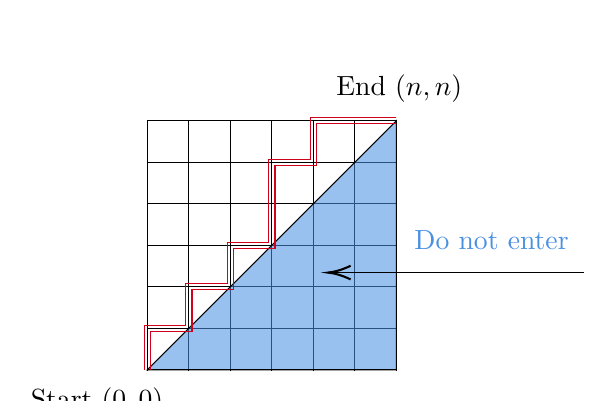
\begin{tikzpicture}[x=0.75pt,y=0.75pt,yscale=-1.,xscale=1.]
    %uncomment if require: \path (0,300); %set diagram left start at 0, and has height of 300
    
    %Shape: Grid [id:dp05086476571583698] 
    \draw  [draw opacity=0] (117,67) -- (237.26,67) -- (237.26,187.51) -- (117,187.51) -- cycle ; \draw   (117,67) -- (117,187.51)(137,67) -- (137,187.51)(157,67) -- (157,187.51)(177,67) -- (177,187.51)(197,67) -- (197,187.51)(217,67) -- (217,187.51)(237,67) -- (237,187.51) ; \draw   (117,67) -- (237.26,67)(117,87) -- (237.26,87)(117,107) -- (237.26,107)(117,127) -- (237.26,127)(117,147) -- (237.26,147)(117,167) -- (237.26,167)(117,187) -- (237.26,187) ; \draw    ;
    %Shape: Right Triangle [id:dp10810256190463985] 
    \draw  [fill={rgb, 255:red, 74; green, 144; blue, 226 }  ,fill opacity=0.56 ] (237,67) -- (117,187) -- (237,187) -- cycle ;
    %Straight Lines [id:da0992245402697518] 
    \draw    (327.46,140.2) -- (206,140.2) ;
    \draw [shift={(204,140.2)}, rotate = 360] [color={rgb, 255:red, 0; green, 0; blue, 0 }  ][line width=0.75]    (10.93,-3.29) .. controls (6.95,-1.4) and (3.31,-0.3) .. (0,0) .. controls (3.31,0.3) and (6.95,1.4) .. (10.93,3.29)   ;
    %Straight Lines [id:da160597462279765] 
    \draw [color={rgb, 255:red, 208; green, 2; blue, 27 }  ,draw opacity=1 ]   (237,68.5) -- (198.5,68.5) -- (198.5,88.5) -- (178.5,88.5) -- (178.5,128.5) -- (158.5,128.5) -- (158.5,134.86) -- (158.5,148.5) -- (138.5,148.5) -- (138.5,168.5) -- (118.5,168.5) -- (118.5,187)(237,65.5) -- (195.5,65.5) -- (195.5,85.5) -- (175.5,85.5) -- (175.5,125.5) -- (155.5,125.5) -- (155.5,134.86) -- (155.5,145.5) -- (135.5,145.5) -- (135.5,165.5) -- (115.5,165.5) -- (115.5,187) ;
    
    % Text Node
    \draw (244.4,118.6) node [anchor=north west][inner sep=0.75pt]  [color={rgb, 255:red, 74; green, 144; blue, 226 }  ,opacity=1 ] [align=left] {Do not enter};
    % Text Node
    \draw (59.6,194.2) node [anchor=north west][inner sep=0.75pt]   [align=left] {Start $\displaystyle ( 0,0)$};
    % Text Node
    \draw (206.8,43.8) node [anchor=north west][inner sep=0.75pt]   [align=left] {End $\displaystyle ( n,n)$};
    
    
    \end{tikzpicture}
    \]

    \textbf{Question:} when is the \textbf{first time} we return to the diagonal? That is, what is the smallest $k\in \{1,2,\dots,n\}$ such that we get $(k,k)$?

    \[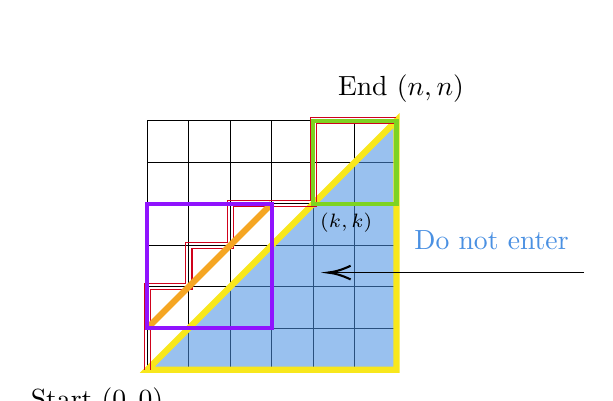
\begin{tikzpicture}[x=0.75pt,y=0.75pt,yscale=-1,xscale=1]
        %uncomment if require: \path (0,300); %set diagram left start at 0, and has height of 300
        
        %Shape: Grid [id:dp43629158818005953] 
        \draw  [draw opacity=0] (117,67) -- (237.26,67) -- (237.26,187.51) -- (117,187.51) -- cycle ; \draw   (117,67) -- (117,187.51)(137,67) -- (137,187.51)(157,67) -- (157,187.51)(177,67) -- (177,187.51)(197,67) -- (197,187.51)(217,67) -- (217,187.51)(237,67) -- (237,187.51) ; \draw   (117,67) -- (237.26,67)(117,87) -- (237.26,87)(117,107) -- (237.26,107)(117,127) -- (237.26,127)(117,147) -- (237.26,147)(117,167) -- (237.26,167)(117,187) -- (237.26,187) ; \draw    ;
        %Shape: Right Triangle [id:dp910522544221946] 
        \draw  [color={rgb, 255:red, 248; green, 231; blue, 28 }  ,draw opacity=1 ][fill={rgb, 255:red, 74; green, 144; blue, 226 }  ,fill opacity=0.56 ][line width=2.25]  (237,67) -- (117,187) -- (237,187) -- cycle ;
        %Straight Lines [id:da5998488809695885] 
        \draw    (327.46,140.2) -- (206,140.2) ;
        \draw [shift={(204,140.2)}, rotate = 360] [color={rgb, 255:red, 0; green, 0; blue, 0 }  ][line width=0.75]    (10.93,-3.29) .. controls (6.95,-1.4) and (3.31,-0.3) .. (0,0) .. controls (3.31,0.3) and (6.95,1.4) .. (10.93,3.29)   ;
        %Straight Lines [id:da8771947101201794] 
        \draw [color={rgb, 255:red, 208; green, 2; blue, 27 }  ,draw opacity=1 ]   (237,68.5) -- (198.5,68.5) -- (198.5,87) -- (198.5,108.5) -- (158.5,108.5) -- (158.5,128.5) -- (138.5,128.5) -- (138.5,148.5) -- (118.5,148.5) -- (118.5,187)(237,65.5) -- (195.5,65.5) -- (195.5,87) -- (195.5,105.5) -- (155.5,105.5) -- (155.5,125.5) -- (135.5,125.5) -- (135.5,145.5) -- (115.5,145.5) -- (115.5,187) ;
        %Straight Lines [id:da3429548095568469] 
        \draw [color={rgb, 255:red, 245; green, 166; blue, 35 }  ,draw opacity=1 ][line width=2.25]    (117,167) -- (177,107) ;
        %Shape: Rectangle [id:dp8136563088561988] 
        \draw  [color={rgb, 255:red, 144; green, 19; blue, 254 }  ,draw opacity=1 ][line width=1.5]  (117,107) -- (177,107) -- (177,167) -- (117,167) -- cycle ;
        %Shape: Rectangle [id:dp9042619059945287] 
        \draw  [color={rgb, 255:red, 126; green, 211; blue, 33 }  ,draw opacity=1 ][line width=1.5]  (197,67) -- (237,67) -- (237,107) -- (197,107) -- cycle ;
        
        % Text Node
        \draw (244.4,118.6) node [anchor=north west][inner sep=0.75pt]  [color={rgb, 255:red, 74; green, 144; blue, 226 }  ,opacity=1 ] [align=left] {Do not enter};
        % Text Node
        \draw (59.6,194.2) node [anchor=north west][inner sep=0.75pt]   [align=left] {Start $\displaystyle ( 0,0)$};
        % Text Node
        \draw (207.6,43.8) node [anchor=north west][inner sep=0.75pt]   [align=left] {End $\displaystyle ( n,n)$};
        % Text Node
        \draw (199,110.4) node [anchor=north west][inner sep=0.75pt]  [font=\scriptsize]  {$( k,k)$};
        
        
        \end{tikzpicture}
        \]

Steps: \begin{enumerate}
    \item $(0,0)\to (0,1)$\hfill 1 way
    \item $(0,1)\to (k-1, k)$ w/o crossing orange line\hfill $C_{k-1}$ ways\sidenote{in the purple square}
    \item $(k-1,k)\to (k,k)$\hfill 1 way
    \item $(0,1)\to (k-1, k)$ w/o crossing yellow line\hfill $C_{n-k}$ ways\sidenote{in the green square}
\end{enumerate}
Hence\sidenote{the Catalan recurrence} \[C_n=\sum_{k=1}^{n} C_{k-1}C_{n-k}\]
And so $C_n=C_0C_{n-1}+\dots + C_{n-1}C_0$.

\eg How many ways to triangulate a convex 47-sided polygon by drawing diagonals? ANS: $D_{47}$!

Examples: 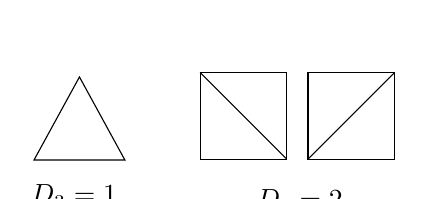
\begin{tikzpicture}[x=0.75pt,y=0.75pt,yscale=-1,xscale=1]
    %uncomment if require: \path (0,300); %set diagram left start at 0, and has height of 300
    
    %Shape: Triangle [id:dp9204215251759331] 
    \draw   (101.88,107) -- (123.76,147) -- (80,147) -- cycle ;
    %Shape: Square [id:dp6960645979215019] 
    \draw   (160,104.86) -- (201.74,104.86) -- (201.74,146.6) -- (160,146.6) -- cycle ;
    %Shape: Square [id:dp8790419330473327] 
    \draw   (212,104.86) -- (253.74,104.86) -- (253.74,146.6) -- (212,146.6) -- cycle ;
    %Straight Lines [id:da10159556423687888] 
    \draw    (160,104.86) -- (201.74,146.6) ;
    %Straight Lines [id:da3782077165685771] 
    \draw    (212,146.6) -- (253.74,104.86) ;
    
    % Text Node
    \draw (77.2,157.8) node [anchor=north west][inner sep=0.75pt]    {$D_{3} =1$};
    % Text Node
    \draw (186,160.2) node [anchor=north west][inner sep=0.75pt]    {$D_{4} =2$};
    
    
    \end{tikzpicture}
\dots    

\textbf{Conjecture:} $D_n=C_{n-2}$
\begin{proof}[Induction proof]
    Base case is done as shown above.

    Inductive step: suppose it works for $n=2,3,\dots,k+1$. Now we want to show $D_{k+2}=C_k$.

    \uline{Case $j$}: we pick a side that has a triangle that goes to the vertex $j$.
    \[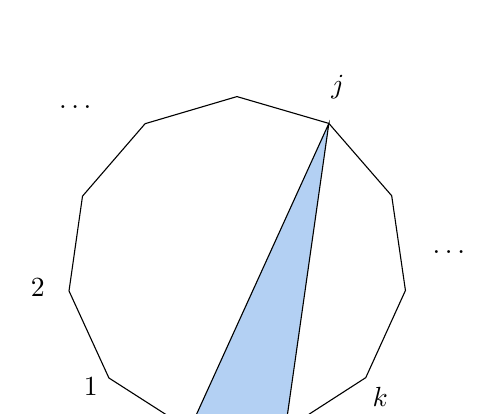
\begin{tikzpicture}[x=0.75pt,y=0.75pt,yscale=-1,xscale=1]
        %uncomment if require: \path (0,300); %set diagram left start at 0, and has height of 300
        
        %Shape: Regular Polygon [id:dp5268773396138595] 
        \draw   (282.94,161.81) -- (263.83,203.81) -- (225.06,228.81) -- (178.92,228.87) -- (140.08,203.98) -- (120.85,162.05) -- (127.35,116.37) -- (157.51,81.46) -- (201.76,68.4) -- (246.05,81.33) -- (276.31,116.16) -- cycle ;
        %Shape: Polygon [id:ds3458377758370945] 
        \draw  [fill={rgb, 255:red, 74; green, 144; blue, 226 }  ,fill opacity=0.42 ] (225.06,228.81) -- (178.92,228.87) -- (246.05,81.33) -- cycle ;
        
        % Text Node
        \draw (126.8,202.6) node [anchor=north west][inner sep=0.75pt]    {$1$};
        % Text Node
        \draw (101.2,154.8) node [anchor=north west][inner sep=0.75pt]    {$2$};
        % Text Node
        \draw (114.8,71.6) node [anchor=north west][inner sep=0.75pt]    {$\dotsc $};
        % Text Node
        \draw (246,56.8) node [anchor=north west][inner sep=0.75pt]    {$j$};
        % Text Node
        \draw (294.8,141.2) node [anchor=north west][inner sep=0.75pt]    {$\dotsc $};
        % Text Node
        \draw (265.83,207.21) node [anchor=north west][inner sep=0.75pt]    {$k$};
        
        
        \end{tikzpicture}
        \]
        On the left, we have a $j+1$ sided polygon and so the number of ways of triangulation is $D_{j+1}=C_{j-1}$.

        On the right, we have a $k-j+2$ sided polygon and so the number of ways of triangulation is $D_{k-j+2}=C_{k-j}$.

        Hence, the number of ways in total is $C_{j-1}\cdot C_{k-j}$. We conclude that \[D_{k+2}=\sum_{j=1}^{k}C_{j-1}C_{k-j}=C_k\] by the Catalan recurrence.
\end{proof}

\subsection{E3 The Catalan bijection}
Suppose a path $(0,0)\to (n,n)$ is \textbf{good} if it does not cross the diagonal $y=x$. We claim that the count of good paths is $\frac{1}{n+1}\binom{2n}{n}$.

Alternatively, we could show that the number of \textbf{bad} paths is $\#\text{ all paths} - \frac{1}{n+1}\binom{2n}{n}$, which means we want to show:\begin{align*}
    \#\text{ \textbf{bad} paths} &= \binom{2n}{n} - \frac{1}{n+1}\binom{2n}{n}\\
    &= \frac{n}{n+1}\binom{2n}{n}\\
    &= \frac{\rt{n}}{\bt{n+1}}\frac{(2n)!}{\rt{n}!\bt{n!}}\\
    &= \frac{(2n)!}{\rt{(n-1)!}\bt{(n+1)!}}\\
    &= {2n\choose n+1}
\end{align*}

A \textbf{bad} path is one that crosses the diagonal $y=x$, but that is equivalent to touching the subdiagonal $y=x-1$.
\[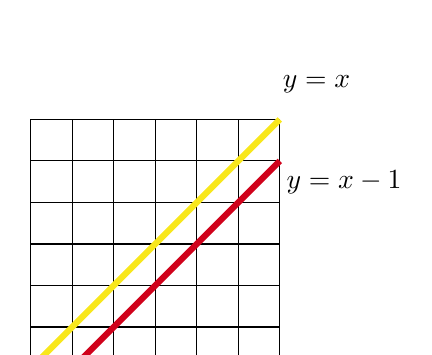
\begin{tikzpicture}[x=0.75pt,y=0.75pt,yscale=-1,xscale=1]
    %uncomment if require: \path (0,300); %set diagram left start at 0, and has height of 300
    
    %Shape: Grid [id:dp8599649850250317] 
    \draw  [draw opacity=0] (137,87) -- (257.26,87) -- (257.26,207.51) -- (137,207.51) -- cycle ; \draw   (137,87) -- (137,207.51)(157,87) -- (157,207.51)(177,87) -- (177,207.51)(197,87) -- (197,207.51)(217,87) -- (217,207.51)(237,87) -- (237,207.51)(257,87) -- (257,207.51) ; \draw   (137,87) -- (257.26,87)(137,107) -- (257.26,107)(137,127) -- (257.26,127)(137,147) -- (257.26,147)(137,167) -- (257.26,167)(137,187) -- (257.26,187)(137,207) -- (257.26,207) ; \draw    ;
    %Straight Lines [id:da23566208454469217] 
    \draw [color={rgb, 255:red, 248; green, 231; blue, 28 }  ,draw opacity=1 ][line width=2.25]    (137,207) -- (227.3,116.7) -- (257,87) ;
    %Straight Lines [id:da10185715014518837] 
    \draw [color={rgb, 255:red, 208; green, 2; blue, 27 }  ,draw opacity=1 ][line width=2.25]    (157,207) -- (257,107) ;
    
    % Text Node
    \draw (257.2,64.4) node [anchor=north west][inner sep=0.75pt]    {$y=x$};
    % Text Node
    \draw (259,110.4) node [anchor=north west][inner sep=0.75pt]    {$y=x-1$};
    
    
    \end{tikzpicture}
    \]

\textbf{Claim}: the number of paths $(0,0)\to (n,n)$ that touch the red line is the same as the number of paths $(0,0)\to (n+1,n-1)$.
\[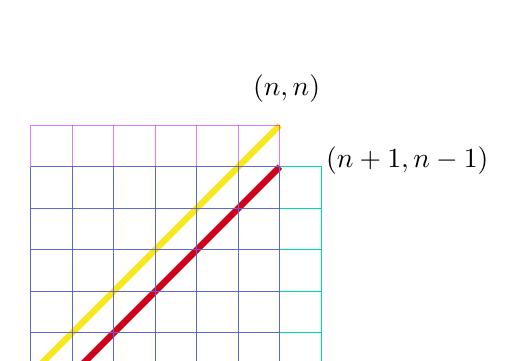
\begin{tikzpicture}[x=0.75pt,y=0.75pt,yscale=-1,xscale=1]
%uncomment if require: \path (0,300); %set diagram left start at 0, and has height of 300

%Straight Lines [id:da23566208454469217] 
\draw [color={rgb, 255:red, 248; green, 231; blue, 28 }  ,draw opacity=1 ][line width=2.25]    (137,207) -- (227.3,116.7) -- (257,87) ;
%Straight Lines [id:da10185715014518837] 
\draw [color={rgb, 255:red, 208; green, 2; blue, 27 }  ,draw opacity=1 ][line width=2.25]    (157,207) -- (257,107) ;
%Shape: Grid [id:dp17881272925547775] 
\draw  [draw opacity=0] (137,107) -- (277.36,107) -- (277.36,207.51) -- (137,207.51) -- cycle ; \draw  [color={rgb, 255:red, 0; green, 217; blue, 161 }  ,draw opacity=1 ] (137,107) -- (137,207.51)(157,107) -- (157,207.51)(177,107) -- (177,207.51)(197,107) -- (197,207.51)(217,107) -- (217,207.51)(237,107) -- (237,207.51)(257,107) -- (257,207.51)(277,107) -- (277,207.51) ; \draw  [color={rgb, 255:red, 0; green, 217; blue, 161 }  ,draw opacity=1 ] (137,107) -- (277.36,107)(137,127) -- (277.36,127)(137,147) -- (277.36,147)(137,167) -- (277.36,167)(137,187) -- (277.36,187)(137,207) -- (277.36,207) ; \draw  [color={rgb, 255:red, 0; green, 217; blue, 161 }  ,draw opacity=1 ]  ;
%Shape: Grid [id:dp45429225148021546] 
\draw  [draw opacity=0] (137,87) -- (257.26,87) -- (257.26,207.51) -- (137,207.51) -- cycle ; \draw  [color={rgb, 255:red, 187; green, 0; blue, 255 }  ,draw opacity=0.51 ] (137,87) -- (137,207.51)(157,87) -- (157,207.51)(177,87) -- (177,207.51)(197,87) -- (197,207.51)(217,87) -- (217,207.51)(237,87) -- (237,207.51)(257,87) -- (257,207.51) ; \draw  [color={rgb, 255:red, 187; green, 0; blue, 255 }  ,draw opacity=0.51 ] (137,87) -- (257.26,87)(137,107) -- (257.26,107)(137,127) -- (257.26,127)(137,147) -- (257.26,147)(137,167) -- (257.26,167)(137,187) -- (257.26,187)(137,207) -- (257.26,207) ; \draw  [color={rgb, 255:red, 187; green, 0; blue, 255 }  ,draw opacity=0.51 ]  ;

% Text Node
\draw (242.8,61.6) node [anchor=north west][inner sep=0.75pt]    {$( n,n)$};
% Text Node
\draw (278,96) node [anchor=north west][inner sep=0.75pt]    {$( n+1,n-1)$};


\end{tikzpicture}
\]
The latter quantity is just $2n\choose n+1$.

We use the following bijection:
\[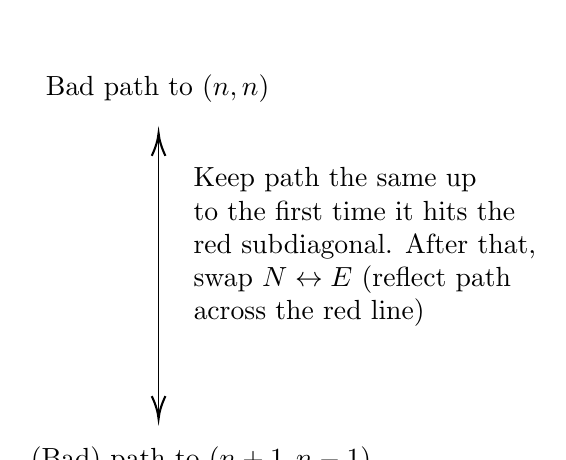
\begin{tikzpicture}[x=0.75pt,y=0.75pt,yscale=-1,xscale=1]
    %uncomment if require: \path (0,300); %set diagram left start at 0, and has height of 300
    
    %Straight Lines [id:da2675009840960558] 
    \draw    (172,67.6) -- (172,201.26) ;
    \draw [shift={(172,203.26)}, rotate = 270] [color={rgb, 255:red, 0; green, 0; blue, 0 }  ][line width=0.75]    (10.93,-3.29) .. controls (6.95,-1.4) and (3.31,-0.3) .. (0,0) .. controls (3.31,0.3) and (6.95,1.4) .. (10.93,3.29)   ;
    \draw [shift={(172,65.6)}, rotate = 90] [color={rgb, 255:red, 0; green, 0; blue, 0 }  ][line width=0.75]    (10.93,-3.29) .. controls (6.95,-1.4) and (3.31,-0.3) .. (0,0) .. controls (3.31,0.3) and (6.95,1.4) .. (10.93,3.29)   ;
    
    % Text Node
    \draw (116.4,36.4) node [anchor=north west][inner sep=0.75pt]   [align=left] {Bad path to $\displaystyle ( n,n)$};
    % Text Node
    \draw (109.2,215.4) node [anchor=north west][inner sep=0.75pt]   [align=left] {(Bad) path to $\displaystyle ( n+1,n-1)$};
    % Text Node
    \draw (187.6,81) node [anchor=north west][inner sep=0.75pt]   [align=left] {Keep path the same up\\to the first time it hits the \\red subdiagonal. After that,\\swap $\displaystyle N\leftrightarrow E$ (reflect path\\across the red line)};
    
    
    \end{tikzpicture}
    \]\sidenote{all paths are bad to $(n+1, n-1)$!}


\section{F Stirling numbers}
\subsection{F1 Table entries 11, 9, 7}
\drawing{0.95\linewidth}{table3-1.pdf}
\begin{itemize}[align=left]
    \item[\circled{11}: ] How many ways to place $s$ distinct objects into $t$ \textbf{unmarked} boxes such that none of the boxes are empty?\sidenote{Distinct objects, identical boxes, $u_i\geq 1$}
    
    $\Leftrightarrow$ organizing $s$ distinct people into $t$ nonempty teams.
    
    We don't know the (closed-form) answer yet, so we temporarily call it $\squig{s}{t}$.

    \eg We have 4 people: A,B,C and D, and we group them into 3 teams. This is the situation $s=4,t=3$. We group:\begin{itemize}
        \item AB|C|D
        \item AC|B|D
        \item AD|B|C
        \item BC|A|D
        \item BD|A|C
        \item CD|A|B
    \end{itemize}
    Therefore, $\squig{4}{3}=6$.

    \item[\circled{9}: ] How many ways to place $s$ distinct objects into $t$ \textbf{named} boxes such that none of the boxes are empty?\sidenote{Distinct objects, distinct boxes, $u_i\geq 1$}
    
    $\Leftrightarrow$ organizing $s$ distinct people into $t$ nonempty teams with different team names.

    Compared with \circled{11}, this gives $t!$ more ways due to the labelling. Therefore, the answer is $t!\squig{s}{t}$.

    \rmk This is the same as counting the number of \textit{surjective} functions $$\{1,2,\dots,s\}\to \{1,2,\dots, t\}$$ we expect some relationship with the quantity $t^s$, which counts all functions.

    \item[\circled{7}: ] How many ways to place $s$ distinct objects into $t$ \textbf{unmarked} boxes?\sidenote{Distinct objects, identical boxes, $u_i\geq 0$. i.e. \circled{11} but boxes can be empty}
    
    Answer: \(\displaystyle \sum_{k=0}^{t}\squig{s}{k}\) where $k$ is the \# of nonempty boxes.
\end{itemize}

\rmk Observe: \[\begin{array}[t]{l|l|l|}
    \cline{2-3}
    u_i\geq 0 & {^{\circled{5}}\quad} t^s&{^{\circled{7}}\quad} \sum_{k=0}^{t}\squig{s}{k}\\[6pt]\cline{2-3}
    u_i\geq 1 & {^{\circled{9}}\quad}t!\squig{s}{t}& {^{\circled{11}}\quad}\squig{s}{t}\\
    \cline{2-3}
\end{array}\]
We can get \circled{9} by multiplying \circled{11} by $t!$, but we cannot get \circled 5 from \circled 7 in the same way due to the empty boxes!

The ways to label boxes in \circled 5 is only $(t)_k$ ways for each \# of nonempty boxes $k$.

\textbf{Conclusion: } \[t^s = \sum_{k=0}^{t}(t)_k\squig{s}k\]
It follows that the quantities $0^s, 1^s,\dots ,s^s$ are \textit{linearly} related to $\squig{s}0, \squig{s}1,\dots, \squig{s}s$.

\eg Let $s=3$. \[
    \begin{bmatrix}
        0\\1\\8\\27
    \end{bmatrix} =
    \begin{bmatrix}
        1&0&0&0\\
        1&1&0&0\\
        1&2&2&0\\
        1&3&6&6
    \end{bmatrix}\cdot
    \begin{bmatrix}
        \squig{3}0\\[6pt]\squig{3}1\\[6pt]\squig{3}2\\[6pt]\squig{3}3
    \end{bmatrix}
    \]
where every entry $(i,j)$ of the matrix is $(i)_j$.

We can invert the matrix to find what $\squig{s}t$ is, but it's computationally quite terrible!

\subsection{F2 Stirling numbers of the second kind}

\defn[Stirling numbers of the second kind] \[\squig{s}t=\text{\# of ways to place $s$ distinct objects into $t$ identical empty boxes}\]

\addlink{Properties of Stirling numbers}
\begin{proposition}\hfill
    \begin{enumerate}
        \item $\squig{s}t=0$ if $t>s$ \hfill too many boxes
        \item $\squig{s}s=1$ \hfill must have object in its own box
        \item $\squig{s}1=1$ for $s\geq 1$ \hfill everything in 1 box
        \item $\squig{s}{s-1}={s\choose 2}$ \hfill which 2 ppl in the team of 2, rest solo
        \item $\squig{s}2 = 2^{s-1}-1$
        
        \item[] Ways:
        \begin{enumerate}
            \item Ask who else among the $s-1$ people are my team, count the possibilities. Subtract the case when everyone is in my team for the other team to be nonempty.
            \item Categorize $s$ people into two \textit{distinct} boxes, which gives us $2^s$ ways. Then, subtract the 2 ways where everyone is in the same box. Finally, since the boxes aren't distinct after all, we divide the result by $2!$.
        \end{enumerate}

        \item $\squig{s}0 = \begin{cases}
            1 &\text{if }s=0\\
            0 &\text{if }s\geq 1
        \end{cases}$
    \end{enumerate}
\end{proposition}
\begin{table}[H]\centering
    \begin{tabular}{l|lllllll|l}
    $s\backslash t$ & 0 & 1 & 2  & 3  & 4  & 5  & 6 & Row sum \\\hline
    0   & \rt{1} & 0 & 0  & 0  & 0  & 0  & 0 & 1       \\
    1   & 0 & \rt{1} & 0  & 0  & 0  & 0  & 0 & 1       \\
    2   & 0 & \rt{1} & \rt{1}  & 0  & 0  & 0  & 0 & 2       \\
    3   & 0 & \rt{1} & \bt{3}  & \rt{1}  & 0  & 0  & 0 & 5       \\
    4   & 0 & \rt{1} & \gt{7}  & \bt{6}  & \rt{1}  & 0  & 0 & 15      \\
    5   & 0 & \rt{1} & \gt{15} & 25 & \bt{10} & \rt{1}  & 0 & 522     \\
    6   & 0 & \rt{1} & \gt{31} & 90 & 65 & \bt{15} & \rt{1} & 203    
    \end{tabular}
\end{table}\sidenote{The row sums are Bell numbers!}

\begin{theorem}
    \[\squig{s}t = t\squig{s-1}t + \squig{s-1}{t-1}\]
\end{theorem}
Understand this as placing people $1,2,\dots, s$ into teams $T_1,\dots,T_t$.

From perspective of person $s$: \begin{itemize}[align=left]
    \item[Case 1: ] Person $s$ is alone, so $\squig{s-1}{t-1}$ ways to organize the rest.
    \item[Case 2: ] Person $s$ is not alone. \begin{itemize}
        \item Organize the rest into $t$ teams, which is $\squig{s-1}t$ ways.
        \item Join one of the teams, which is $t$ ways.
    \end{itemize}
\end{itemize}
Add the two cases.

\subsection{F3 Stirling numbers of the first kind}
\defn[Stirling numbers of the first kind] \[{n\brack k} = \# \text{ of ways of seating $n$ people at $k$ circular tables (no empty table)}\]

In general, ${n\brack k} \geq \squig{n}k$ (usually a lot bigger) because of the extra choices needed to seat the $k$ teams at tables.

\eg We let $n=5,k=2$.
\begin{itemize}[align=left]
    \item[Case 1: ] split into 3+2 \[\begin{tikzpicture}[x=0.75pt,y=0.75pt,yscale=-1,xscale=1]
        %uncomment if require: \path (0,300); %set diagram left start at 0, and has height of 300
        
        %Shape: Circle [id:dp8811209584476829] 
        \draw   (100,148.63) .. controls (100,128.4) and (116.4,112) .. (136.63,112) .. controls (156.86,112) and (173.26,128.4) .. (173.26,148.63) .. controls (173.26,168.86) and (156.86,185.26) .. (136.63,185.26) .. controls (116.4,185.26) and (100,168.86) .. (100,148.63) -- cycle ;
        %Shape: Circle [id:dp0797589490382733] 
        \draw   (234,167.13) .. controls (234,154.91) and (243.91,145) .. (256.13,145) .. controls (268.35,145) and (278.26,154.91) .. (278.26,167.13) .. controls (278.26,179.35) and (268.35,189.26) .. (256.13,189.26) .. controls (243.91,189.26) and (234,179.35) .. (234,167.13) -- cycle ;
        
        % Text Node
        \draw (96,96.4) node [anchor=north west][inner sep=0.75pt]    {$1$};
        % Text Node
        \draw (180,119.4) node [anchor=north west][inner sep=0.75pt]    {$2$};
        % Text Node
        \draw (118,192.4) node [anchor=north west][inner sep=0.75pt]    {$3$};
        % Text Node
        \draw (250,123.4) node [anchor=north west][inner sep=0.75pt]    {$4$};
        % Text Node
        \draw (251,196.4) node [anchor=north west][inner sep=0.75pt]    {$5$};
        
        
        \end{tikzpicture}
        \]
        \begin{itemize}
            \item Choose two people to sit at the table for two: $5\choose 2$=10
            \item Place around the circular tables: $(3-1)!\times(2-1)!=2$
        \end{itemize}
    \item[Case 2: ] split into 4+1 \[\begin{tikzpicture}[x=0.75pt,y=0.75pt,yscale=-1,xscale=1]
        %uncomment if require: \path (0,300); %set diagram left start at 0, and has height of 300
        
        %Shape: Circle [id:dp8811209584476829] 
        \draw   (100,148.63) .. controls (100,128.4) and (116.4,112) .. (136.63,112) .. controls (156.86,112) and (173.26,128.4) .. (173.26,148.63) .. controls (173.26,168.86) and (156.86,185.26) .. (136.63,185.26) .. controls (116.4,185.26) and (100,168.86) .. (100,148.63) -- cycle ;
        %Shape: Circle [id:dp0797589490382733] 
        \draw   (236,141.13) .. controls (236,128.91) and (245.91,119) .. (258.13,119) .. controls (270.35,119) and (280.26,128.91) .. (280.26,141.13) .. controls (280.26,153.35) and (270.35,163.26) .. (258.13,163.26) .. controls (245.91,163.26) and (236,153.35) .. (236,141.13) -- cycle ;
        
        % Text Node
        \draw (90,99.4) node [anchor=north west][inner sep=0.75pt]    {$1$};
        % Text Node
        \draw (171,100.4) node [anchor=north west][inner sep=0.75pt]    {$2$};
        % Text Node
        \draw (89,176.4) node [anchor=north west][inner sep=0.75pt]    {$3$};
        % Text Node
        \draw (170,174.4) node [anchor=north west][inner sep=0.75pt]    {$4$};
        % Text Node
        \draw (253,170.4) node [anchor=north west][inner sep=0.75pt]    {$5$};
        
        
        \end{tikzpicture}
        \]
        \begin{itemize}
            \item Choose 1 person to sit alone: 5
            \item Place around circular table: $(4-1)!=6$
        \end{itemize}
\end{itemize}
Hence, the total ways is ${5\brack 2}=20+30=50$.

\rmk The first task of each case gives us $\squig{5}2=10+5=15$. We can get crude bounds: \[2\squig{5}2<{5\brack 2}<6\squig{5}2\]

\begin{proposition}\hfill
    \begin{enumerate}
        \item \({n\brack k}=0\) if $k>n$: too many tables
        \item \({n\brack 0}=0\) if $n\geq 1$: not enough tables
        \item \({n\brack n}=1\): one person per table
        \item \({n\brack 1}=(n-1)!\) for $n\geq 1$: simple circular permutation
        \item \({n\brack n-1}={n\choose 2}\): which 2 sit at the table for 2
    \end{enumerate}
\end{proposition}

\subsubsection{Table of values of \(n\brack k\)}
\begin{table}[H]\centering
    \begin{tabular}{l|lllllll|l|l}
    $s\backslash t$ & 0 & 1 & 2  & 3  & 4  & 5  & 6 & Row sum & Alternating sum\\\hline
    0   & \rt{1} & 0 & 0  & 0  & 0  & 0  & 0 & 1 & 1      \\
    1   & 0 & \rt{1} & 0  & 0  & 0  & 0  & 0 & 1 & -1      \\
    2   & 0 & \bt{1} & \rt{1}  & 0  & 0  & 0  & 0 & 2 & 0      \\
    3   & 0 & \pt{2} & \bt{3}  & \rt{1}  & 0  & 0  & 0 & 6  &0     \\
    4   & 0 & \pt{6} & 11  & \bt{6}  & \rt{1}  & 0  & 0 & 24  &0    \\
    5   & 0 & \pt{24} & 50 & 35 & \bt{10} & \rt{1}  & 0 & 120  &0   \\
    6   & 0 & \pt{120} & 274 & 225 & 85 & \bt{15} & \rt{1} & 720 &0   
    \end{tabular}
\end{table}

\addlink{Recurrence of Stirling numbers of the first kind}
\begin{theorem}
    \[{n\brack k}=(n-1){n-1\brack k}+{n-1\brack k-1}\]
\end{theorem}
\begin{proof}
    Consider from the perspective of yourself. We seat $n$ people at $k$ table.\begin{itemize}
        \item You sit alone: \begin{itemize}
            \item You seat the rest of the people at $k-1$ tables: $n-1\brack k-1$ ways
            \item Claim the last table by yourself
        \end{itemize}
        \item You don't sit alone: \begin{itemize}
            \item Seat the rest of the people at $k$ tables: $n-1\brack k$ ways
            \item You sit to the left of somebody: $n-1$ ways
        \end{itemize}
    \end{itemize}
\end{proof}

\begin{theorem}
    \[\sum_{k=0}^{n}{n\brack k}=n!\]
\end{theorem}
\begin{proof}[Proof outline]
    We claim: \begin{align*}
        \text{LHS} &= \#\text{ ways to seat $n$ people at circular tables}\\
        \text{RHS} &= \#\text{ permutations of }[n]=\{1,2,\dots,n\}
    \end{align*}
    and there is a bijections between ways to seat $n$ people at circular tables and permutations of $[n]$. \sidenote{Consider the elements of $S_n$.}
\end{proof}

\begin{theorem}
    \[\sum_{k=0}^{n}(-1)^k{n\brack k} = \begin{cases}
        1 & n=0\\
        -1 & n=1\\
        0 & n\geq 2
    \end{cases}\]
\end{theorem}
\begin{proof}[Sketch]
    We are effectively counting the permutations with $\pm$ sign according to whether the number of cycles is even or odd.

    It turns out: \[(-1)^{\#\text{ cycles}} = (-1)^{n}\cdot (\text{sign of permutation})\] and follows that \[LHS = (-1)^{n}\cdot \det \begin{bmatrix}
        1&1&\dots&1\\
        1&1&\dots&1\\
        \vdots&\vdots&\ddots &\vdots\\
        1&1&\dots&1
    \end{bmatrix}\]

    Since $\det[]=1$, $\det[1]=1$ and $\det=0$ otherwise, we are done.
\end{proof}

\begin{theorem}
    \[1+\frac{1}{2}+\frac{1}{3}+\dots+\frac{1}{n} = \frac{{n+1\brack 2}}{n!}\]
\end{theorem}
\begin{proof}[Proof by induction]
    True for: \begin{align*}
        1 &= \frac{1}{1}\\
        1+\frac{1}{2} &= \frac{3}{2!}\\
        1+\frac{1}{2} + \frac{1}{3} &= \frac{11}{3!}
    \end{align*}
    Then, suppose true for $n=k-1$. Then \begin{align*}
        1+\frac{1}{2}+\dots+\frac{1}{k-1}+\frac{1}{n}&=\frac{{k\brack 2}}{(k-1)!}+\frac{1}{k}\\
        &= \frac{k{k\brack 2}+(k-1)!}{k!}\\
        &= \frac{k{k\brack 2}+{k\brack 1}}{k!}\\
        &= \frac{{k+1\brack 2}}{k!}
    \end{align*}
\end{proof}

\section{G The inclusion-exclusion (IE) principle}
\textit{Sometimes AND is easy, but OR is difficult.} This is when IE can help.

It is really about handling Venn diagrams or indicator functions.

\subsection{G1 Introduction}
\eg How many anagrams of MATHFUN have \textbf{neither} of the substrings MATH or FUN?

Let $S=\{\text{anagrams of MATHFUN}\}, A_{MATH}=\{\text{anagrams of MATH}\}$ and $A_{FUN}=\{\text{anagrams of FUN}\}$. We can draw the following Venn diagram:
\[
    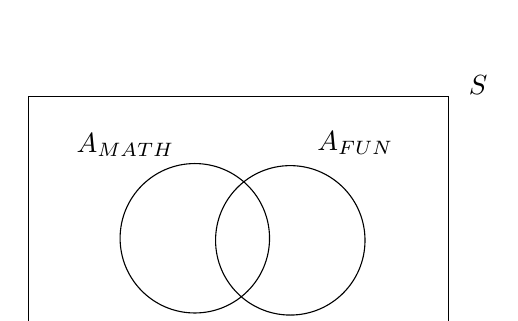
\begin{tikzpicture}[x=0.75pt,y=0.75pt,yscale=-1,xscale=1]
        %uncomment if require: \path (0,300); %set diagram left start at 0, and has height of 300
        
        %Shape: Rectangle [id:dp38802884054568243] 
        \draw   (100,119) -- (302.59,119) -- (302.59,234.76) -- (100,234.76) -- cycle ;
        %Shape: Circle [id:dp7635323589331515] 
        \draw   (190.26,188.26) .. controls (190.26,168.37) and (206.37,152.26) .. (226.26,152.26) .. controls (246.14,152.26) and (262.26,168.37) .. (262.26,188.26) .. controls (262.26,208.14) and (246.14,224.26) .. (226.26,224.26) .. controls (206.37,224.26) and (190.26,208.14) .. (190.26,188.26) -- cycle ;
        %Shape: Circle [id:dp7030560583467587] 
        \draw   (144.26,187.26) .. controls (144.26,167.37) and (160.37,151.26) .. (180.26,151.26) .. controls (200.14,151.26) and (216.26,167.37) .. (216.26,187.26) .. controls (216.26,207.14) and (200.14,223.26) .. (180.26,223.26) .. controls (160.37,223.26) and (144.26,207.14) .. (144.26,187.26) -- cycle ;
        
        % Text Node
        \draw (311,107.4) node [anchor=north west][inner sep=0.75pt]    {$S$};
        % Text Node
        \draw (122,135.4) node [anchor=north west][inner sep=0.75pt]    {$A_{MATH}$};
        % Text Node
        \draw (238,134.4) node [anchor=north west][inner sep=0.75pt]    {$A_{FUN}$};
        
        
        \end{tikzpicture}      
\]
Where:
\[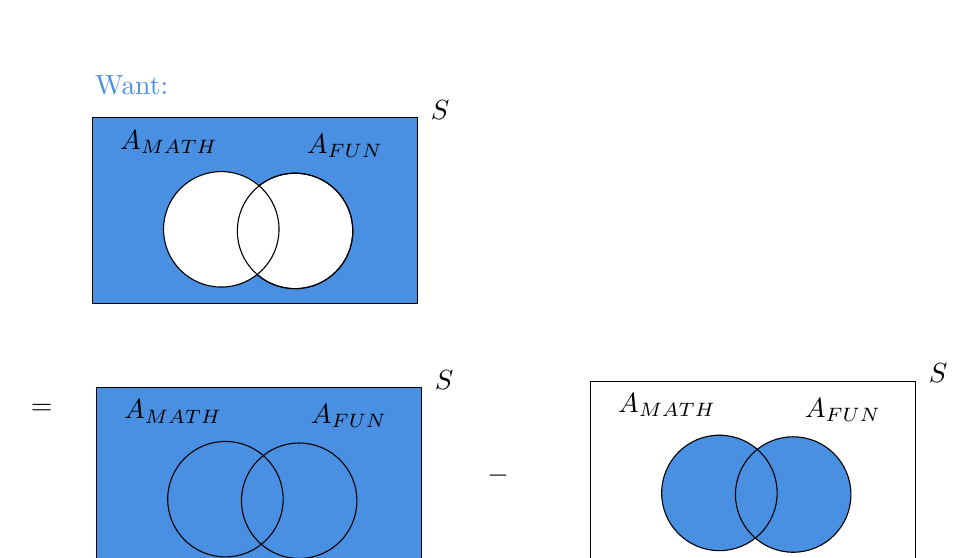
\begin{tikzpicture}[x=0.75pt,y=0.75pt,yscale=-1,xscale=1]
    %uncomment if require: \path (0,300); %set diagram left start at 0, and has height of 300
    
    %Shape: Rectangle [id:dp4731520072226425] 
    \draw  [fill={rgb, 255:red, 74; green, 144; blue, 226 }  ,fill opacity=1 ] (55,36.82) -- (211.53,36.82) -- (211.53,126.26) -- (55,126.26) -- cycle ;
    %Shape: Ellipse [id:dp805463853475932] 
    \draw  [fill={rgb, 255:red, 255; green, 255; blue, 255 }  ,fill opacity=1 ] (124.74,91.33) .. controls (124.74,75.97) and (137.19,63.51) .. (152.55,63.51) .. controls (167.92,63.51) and (180.37,75.97) .. (180.37,91.33) .. controls (180.37,106.69) and (167.92,119.14) .. (152.55,119.14) .. controls (137.19,119.14) and (124.74,106.69) .. (124.74,91.33) -- cycle ;
    %Shape: Circle [id:dp23502392099226754] 
    \draw  [fill={rgb, 255:red, 255; green, 255; blue, 255 }  ,fill opacity=1 ] (89.19,90.56) .. controls (89.19,75.19) and (101.65,62.74) .. (117.01,62.74) .. controls (132.37,62.74) and (144.83,75.19) .. (144.83,90.56) .. controls (144.83,105.92) and (132.37,118.37) .. (117.01,118.37) .. controls (101.65,118.37) and (89.19,105.92) .. (89.19,90.56) -- cycle ;
    %Shape: Ellipse [id:dp335874410640951] 
    \draw   (124.74,91.33) .. controls (124.74,75.97) and (137.19,63.51) .. (152.55,63.51) .. controls (167.92,63.51) and (180.37,75.97) .. (180.37,91.33) .. controls (180.37,106.69) and (167.92,119.14) .. (152.55,119.14) .. controls (137.19,119.14) and (124.74,106.69) .. (124.74,91.33) -- cycle ;
    %Shape: Rectangle [id:dp7196978245248316] 
    \draw  [fill={rgb, 255:red, 74; green, 144; blue, 226 }  ,fill opacity=1 ] (57,166.82) -- (213.53,166.82) -- (213.53,256.26) -- (57,256.26) -- cycle ;
    %Shape: Ellipse [id:dp9282199642226638] 
    \draw   (126.74,221.33) .. controls (126.74,205.97) and (139.19,193.51) .. (154.55,193.51) .. controls (169.92,193.51) and (182.37,205.97) .. (182.37,221.33) .. controls (182.37,236.69) and (169.92,249.14) .. (154.55,249.14) .. controls (139.19,249.14) and (126.74,236.69) .. (126.74,221.33) -- cycle ;
    %Shape: Circle [id:dp035150929059933445] 
    \draw   (91.19,220.56) .. controls (91.19,205.19) and (103.65,192.74) .. (119.01,192.74) .. controls (134.37,192.74) and (146.83,205.19) .. (146.83,220.56) .. controls (146.83,235.92) and (134.37,248.37) .. (119.01,248.37) .. controls (103.65,248.37) and (91.19,235.92) .. (91.19,220.56) -- cycle ;
    %Shape: Rectangle [id:dp5897864622911284] 
    \draw   (295,163.82) -- (451.53,163.82) -- (451.53,253.26) -- (295,253.26) -- cycle ;
    %Shape: Ellipse [id:dp2470635995527788] 
    \draw  [draw opacity=0][fill={rgb, 255:red, 74; green, 144; blue, 226 }  ,fill opacity=1 ] (364.74,218.33) .. controls (364.74,202.97) and (377.19,190.51) .. (392.55,190.51) .. controls (407.92,190.51) and (420.37,202.97) .. (420.37,218.33) .. controls (420.37,233.69) and (407.92,246.14) .. (392.55,246.14) .. controls (377.19,246.14) and (364.74,233.69) .. (364.74,218.33) -- cycle ;
    %Shape: Circle [id:dp3814434746266411] 
    \draw  [fill={rgb, 255:red, 74; green, 144; blue, 226 }  ,fill opacity=1 ] (329.19,217.56) .. controls (329.19,202.19) and (341.65,189.74) .. (357.01,189.74) .. controls (372.37,189.74) and (384.83,202.19) .. (384.83,217.56) .. controls (384.83,232.92) and (372.37,245.37) .. (357.01,245.37) .. controls (341.65,245.37) and (329.19,232.92) .. (329.19,217.56) -- cycle ;
    %Shape: Ellipse [id:dp249347285064065] 
    \draw   (364.74,218.33) .. controls (364.74,202.97) and (377.19,190.51) .. (392.55,190.51) .. controls (407.92,190.51) and (420.37,202.97) .. (420.37,218.33) .. controls (420.37,233.69) and (407.92,246.14) .. (392.55,246.14) .. controls (377.19,246.14) and (364.74,233.69) .. (364.74,218.33) -- cycle ;
    
    % Text Node
    \draw (216.67,27.13) node [anchor=north west][inner sep=0.75pt]    {$S$};
    % Text Node
    \draw (66.97,41.53) node [anchor=north west][inner sep=0.75pt]    {$A_{MATH}$};
    % Text Node
    \draw (156.97,43.76) node [anchor=north west][inner sep=0.75pt]    {$A_{FUN}$};
    % Text Node
    \draw (55,15) node [anchor=north west][inner sep=0.75pt]  [color={rgb, 255:red, 74; green, 144; blue, 226 }  ,opacity=1 ] [align=left] {Want:};
    % Text Node
    \draw (24,173.4) node [anchor=north west][inner sep=0.75pt]    {$=$};
    % Text Node
    \draw (218.67,157.13) node [anchor=north west][inner sep=0.75pt]    {$S$};
    % Text Node
    \draw (68.97,171.53) node [anchor=north west][inner sep=0.75pt]    {$A_{MATH}$};
    % Text Node
    \draw (158.97,173.76) node [anchor=north west][inner sep=0.75pt]    {$A_{FUN}$};
    % Text Node
    \draw (244,203.4) node [anchor=north west][inner sep=0.75pt]    {$-$};
    % Text Node
    \draw (456.67,154.13) node [anchor=north west][inner sep=0.75pt]    {$S$};
    % Text Node
    \draw (306.97,168.53) node [anchor=north west][inner sep=0.75pt]    {$A_{MATH}$};
    % Text Node
    \draw (396.97,170.76) node [anchor=north west][inner sep=0.75pt]    {$A_{FUN}$};
    
    
    \end{tikzpicture}
    \]
Note that \[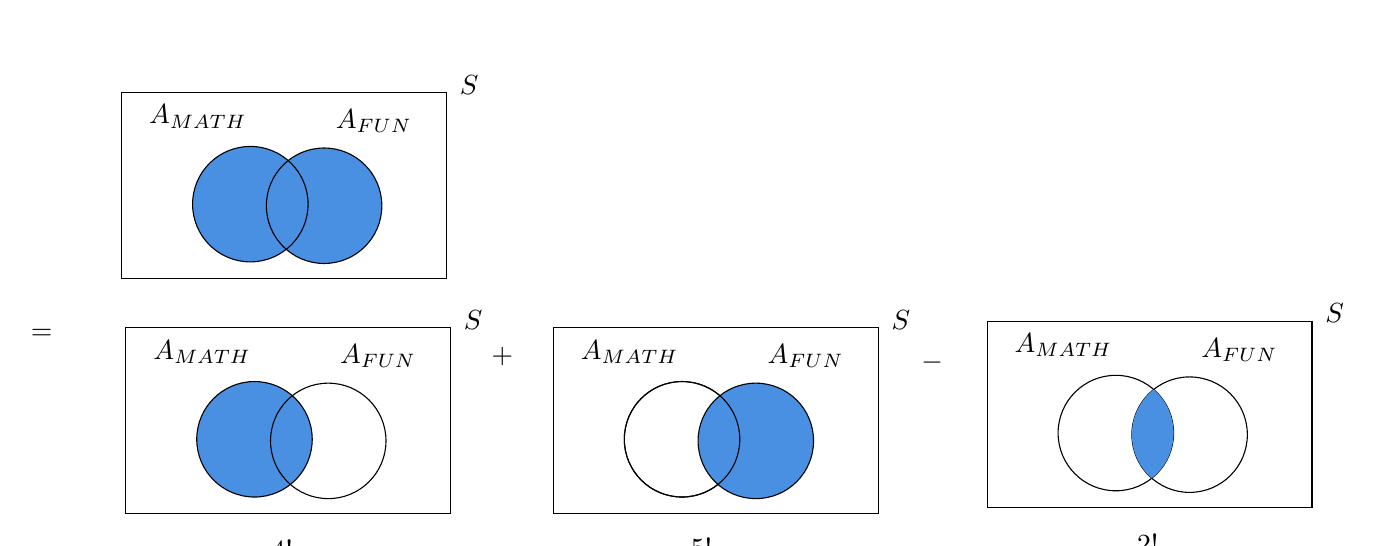
\begin{tikzpicture}[x=0.75pt,y=0.75pt,yscale=-1,xscale=1]
    %uncomment if require: \path (0,300); %set diagram left start at 0, and has height of 300
    
    %Shape: Rectangle [id:dp5763862696816828] 
    \draw   (57,24.81) -- (213.53,24.81) -- (213.53,114.25) -- (57,114.25) -- cycle ;
    %Shape: Ellipse [id:dp05980937945318687] 
    \draw  [draw opacity=0][fill={rgb, 255:red, 74; green, 144; blue, 226 }  ,fill opacity=1 ] (126.74,79.32) .. controls (126.74,63.96) and (139.19,51.5) .. (154.55,51.5) .. controls (169.92,51.5) and (182.37,63.96) .. (182.37,79.32) .. controls (182.37,94.68) and (169.92,107.13) .. (154.55,107.13) .. controls (139.19,107.13) and (126.74,94.68) .. (126.74,79.32) -- cycle ;
    %Shape: Circle [id:dp4971746073701815] 
    \draw  [fill={rgb, 255:red, 74; green, 144; blue, 226 }  ,fill opacity=1 ] (91.19,78.55) .. controls (91.19,63.18) and (103.65,50.73) .. (119.01,50.73) .. controls (134.37,50.73) and (146.83,63.18) .. (146.83,78.55) .. controls (146.83,93.91) and (134.37,106.36) .. (119.01,106.36) .. controls (103.65,106.36) and (91.19,93.91) .. (91.19,78.55) -- cycle ;
    %Shape: Ellipse [id:dp8356592235586819] 
    \draw   (126.74,79.32) .. controls (126.74,63.96) and (139.19,51.5) .. (154.55,51.5) .. controls (169.92,51.5) and (182.37,63.96) .. (182.37,79.32) .. controls (182.37,94.68) and (169.92,107.13) .. (154.55,107.13) .. controls (139.19,107.13) and (126.74,94.68) .. (126.74,79.32) -- cycle ;
    %Shape: Rectangle [id:dp11788061120560678] 
    \draw   (59,138.09) -- (215.53,138.09) -- (215.53,227.54) -- (59,227.54) -- cycle ;
    %Shape: Circle [id:dp742012315778511] 
    \draw  [fill={rgb, 255:red, 74; green, 144; blue, 226 }  ,fill opacity=1 ] (93.19,191.83) .. controls (93.19,176.47) and (105.65,164.01) .. (121.01,164.01) .. controls (136.37,164.01) and (148.83,176.47) .. (148.83,191.83) .. controls (148.83,207.19) and (136.37,219.65) .. (121.01,219.65) .. controls (105.65,219.65) and (93.19,207.19) .. (93.19,191.83) -- cycle ;
    %Shape: Ellipse [id:dp6649356813499605] 
    \draw   (128.74,192.6) .. controls (128.74,177.24) and (141.19,164.79) .. (156.55,164.79) .. controls (171.92,164.79) and (184.37,177.24) .. (184.37,192.6) .. controls (184.37,207.96) and (171.92,220.42) .. (156.55,220.42) .. controls (141.19,220.42) and (128.74,207.96) .. (128.74,192.6) -- cycle ;
    %Shape: Rectangle [id:dp3887579247680759] 
    \draw   (265,138.09) -- (421.53,138.09) -- (421.53,227.54) -- (265,227.54) -- cycle ;
    %Shape: Circle [id:dp654203325014189] 
    \draw   (299.19,191.83) .. controls (299.19,176.47) and (311.65,164.01) .. (327.01,164.01) .. controls (342.37,164.01) and (354.83,176.47) .. (354.83,191.83) .. controls (354.83,207.19) and (342.37,219.65) .. (327.01,219.65) .. controls (311.65,219.65) and (299.19,207.19) .. (299.19,191.83) -- cycle ;
    %Shape: Ellipse [id:dp8217413530832947] 
    \draw  [fill={rgb, 255:red, 74; green, 144; blue, 226 }  ,fill opacity=1 ] (334.74,192.6) .. controls (334.74,177.24) and (347.19,164.79) .. (362.55,164.79) .. controls (377.92,164.79) and (390.37,177.24) .. (390.37,192.6) .. controls (390.37,207.96) and (377.92,220.42) .. (362.55,220.42) .. controls (347.19,220.42) and (334.74,207.96) .. (334.74,192.6) -- cycle ;
    %Shape: Circle [id:dp6982878886377983] 
    \draw   (299.19,191.83) .. controls (299.19,176.47) and (311.65,164.01) .. (327.01,164.01) .. controls (342.37,164.01) and (354.83,176.47) .. (354.83,191.83) .. controls (354.83,207.19) and (342.37,219.65) .. (327.01,219.65) .. controls (311.65,219.65) and (299.19,207.19) .. (299.19,191.83) -- cycle ;
    %Shape: Rectangle [id:dp08306957984161611] 
    \draw   (474,135.09) -- (630.53,135.09) -- (630.53,224.54) -- (474,224.54) -- cycle ;
    %Shape: Circle [id:dp8242567873480398] 
    \draw   (508.19,188.83) .. controls (508.19,173.47) and (520.65,161.01) .. (536.01,161.01) .. controls (551.37,161.01) and (563.83,173.47) .. (563.83,188.83) .. controls (563.83,204.19) and (551.37,216.65) .. (536.01,216.65) .. controls (520.65,216.65) and (508.19,204.19) .. (508.19,188.83) -- cycle ;
    %Shape: Ellipse [id:dp5235224069392781] 
    \draw   (543.74,189.6) .. controls (543.74,174.24) and (556.19,161.79) .. (571.55,161.79) .. controls (586.92,161.79) and (599.37,174.24) .. (599.37,189.6) .. controls (599.37,204.96) and (586.92,217.42) .. (571.55,217.42) .. controls (556.19,217.42) and (543.74,204.96) .. (543.74,189.6) -- cycle ;
    %Shape: Path Data [id:dp3308211305694244] 
    \draw  [draw opacity=0][fill={rgb, 255:red, 74; green, 144; blue, 226 }  ,fill opacity=1 ] (563.83,188.83) .. controls (563.83,197.65) and (559.72,205.51) .. (553.32,210.61) .. controls (547.45,205.51) and (543.74,197.99) .. (543.74,189.6) .. controls (543.74,180.78) and (547.84,172.92) .. (554.25,167.82) .. controls (560.12,172.92) and (563.83,180.44) .. (563.83,188.83) -- cycle ;
    
    % Text Node
    \draw (218.67,15.12) node [anchor=north west][inner sep=0.75pt]    {$S$};
    % Text Node
    \draw (68.97,29.52) node [anchor=north west][inner sep=0.75pt]    {$A_{MATH}$};
    % Text Node
    \draw (158.97,31.75) node [anchor=north west][inner sep=0.75pt]    {$A_{FUN}$};
    % Text Node
    \draw (12,137.4) node [anchor=north west][inner sep=0.75pt]    {$=$};
    % Text Node
    \draw (220.67,128.4) node [anchor=north west][inner sep=0.75pt]    {$S$};
    % Text Node
    \draw (70.97,142.81) node [anchor=north west][inner sep=0.75pt]    {$A_{MATH}$};
    % Text Node
    \draw (160.97,145.03) node [anchor=north west][inner sep=0.75pt]    {$A_{FUN}$};
    % Text Node
    \draw (426.67,128.4) node [anchor=north west][inner sep=0.75pt]    {$S$};
    % Text Node
    \draw (276.97,142.81) node [anchor=north west][inner sep=0.75pt]    {$A_{MATH}$};
    % Text Node
    \draw (366.97,145.03) node [anchor=north west][inner sep=0.75pt]    {$A_{FUN}$};
    % Text Node
    \draw (635.67,125.4) node [anchor=north west][inner sep=0.75pt]    {$S$};
    % Text Node
    \draw (485.97,139.81) node [anchor=north west][inner sep=0.75pt]    {$A_{MATH}$};
    % Text Node
    \draw (575.97,142.03) node [anchor=north west][inner sep=0.75pt]    {$A_{FUN}$};
    % Text Node
    \draw (234,146.4) node [anchor=north west][inner sep=0.75pt]    {$+$};
    % Text Node
    \draw (441,149.4) node [anchor=north west][inner sep=0.75pt]    {$-$};
    % Text Node
    \draw (128,239.4) node [anchor=north west][inner sep=0.75pt]    {$4!$};
    % Text Node
    \draw (330,238.4) node [anchor=north west][inner sep=0.75pt]    {$5!$};
    % Text Node
    \draw (545,236.4) node [anchor=north west][inner sep=0.75pt]    {$2!$};
    
    
    \end{tikzpicture}
    \]
And hence, the answer is $7!-(4!+5!-2!)=4898$.

\subsubsection{Indicator functions}
These are $\{0,1\}$-valued functions on $S$.
\eg Let: \begin{align*}
    \1_s(x) &=1 \text{\quad for all anagrams of $x$}\\
    \1_{MATH}(x) &= \begin{cases}
        1 & \text{if $x$ contains MATH}\\
        0 & \text{otherwise}
    \end{cases}\\
    \1_{FUN}(x) &= \begin{cases}
        1 & \text{if $x$ contains FUN}\\
        0 & \text{otherwise}
    \end{cases}\\
\end{align*}

\begin{proposition} Key facts about indicator functions:
    \begin{itemize}[align=left]
        \item[AND:] $$\1_{A\cap B}=\1_A\1_B$$
        \item[COMPLEMENT:] $$\1_{A}^c = 1-\1_A$$
        \item[OR:] \begin{align*}
            \1_{A\cup B} &= 1- \1_{A^c\cap B^c}\\
            &= 1-\1_{A^c}\1_{B^c}\\
            &= 1-(1-\1_A)(1-\1_B)\\
            &= \1_A+\1_B-\1_{A\cap B}
        \end{align*}  
    \end{itemize}
\end{proposition}

So we get the same formula for the previous example: \[\1_{\text{MATH or FUN}} = \1_{MATH} + \1_{FUN} - \1_{\text{MATH and FUN}}\qquad (*)\]

\defn For any function $f:S\to \R$, we can define \[\int f = \sum_{x\in S} f(x)\] For indicator functions,\[\int {\1_A} = \sum_{x\in S}\begin{cases}
    1 & x\in A\\ 0 & x\not \in A
\end{cases} = \sum_{x\in A} 1 = |A|\] we get the cardinality of $A$.

Therefore, we integrate both sides of $(*)$ and get the cardinality of $A_{MATH}\cup A_{FUN}$.

\eg How many anagrams of MATHISFUN do contain at least one of MATH, IS or FUN?

\textbf{Method 1:} \[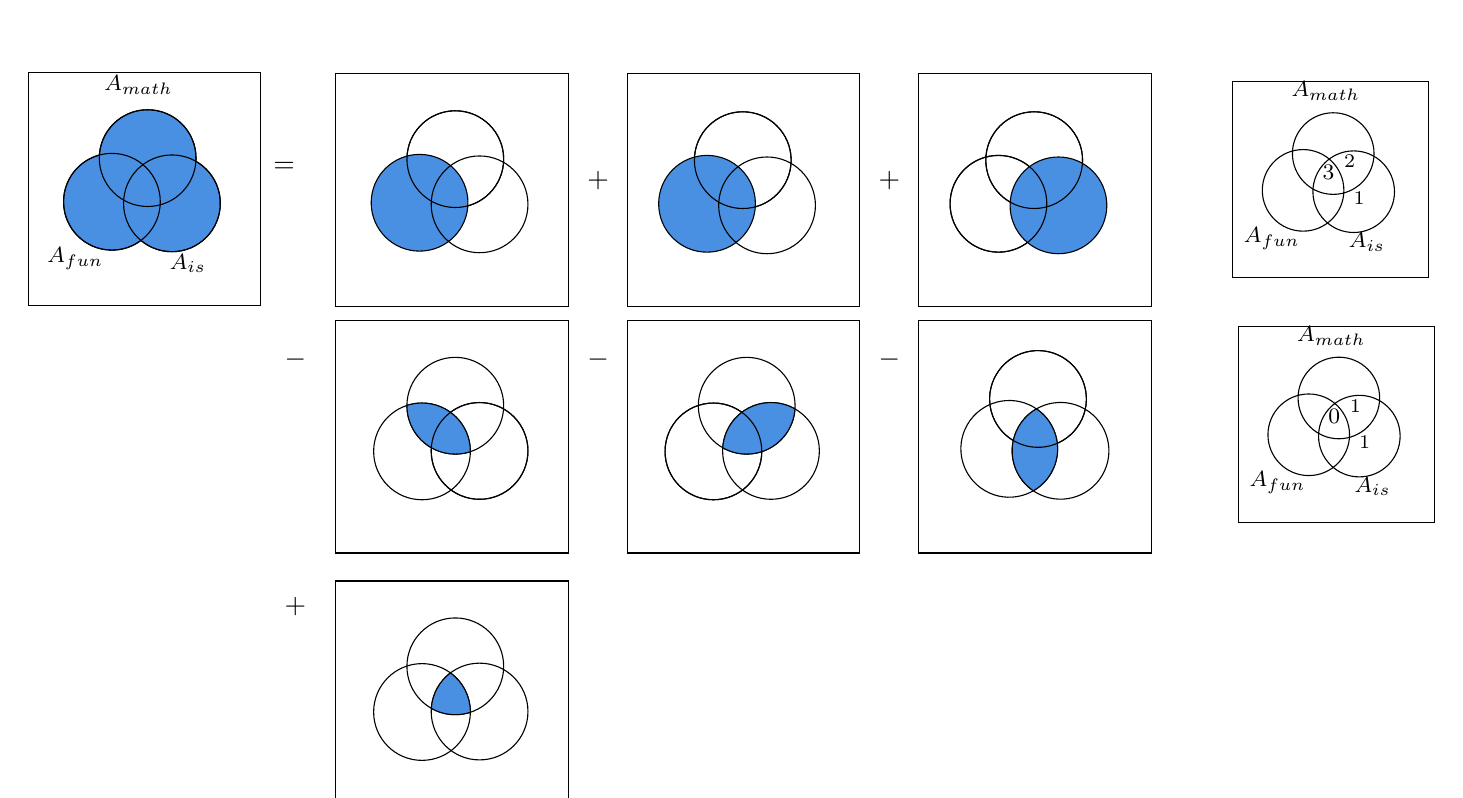
\begin{tikzpicture}[x=0.75pt,y=0.75pt,yscale=-1.08,xscale=1.08]
    %uncomment if require: \path (0,384); %set diagram left start at 0, and has height of 384
    
    %Shape: Rectangle [id:dp1385864763397704] 
    \draw   (560,13.48) -- (647.49,13.48) -- (647.49,100.97) -- (560,100.97) -- cycle ;
    %Shape: Ellipse [id:dp6084455910460216] 
    \draw   (586.73,45.56) .. controls (586.73,35.51) and (594.88,27.36) .. (604.93,27.36) .. controls (614.98,27.36) and (623.13,35.51) .. (623.13,45.56) .. controls (623.13,55.61) and (614.98,63.76) .. (604.93,63.76) .. controls (594.88,63.76) and (586.73,55.61) .. (586.73,45.56) -- cycle ;
    %Shape: Ellipse [id:dp9503734948864271] 
    \draw   (573.29,61.97) .. controls (573.29,51.93) and (581.44,43.78) .. (591.49,43.78) .. controls (601.54,43.78) and (609.68,51.93) .. (609.68,61.97) .. controls (609.68,72.02) and (601.54,80.17) .. (591.49,80.17) .. controls (581.44,80.17) and (573.29,72.02) .. (573.29,61.97) -- cycle ;
    %Shape: Ellipse [id:dp3309171920842988] 
    \draw   (595.87,62.57) .. controls (595.87,52.52) and (604.01,44.37) .. (614.06,44.37) .. controls (624.11,44.37) and (632.26,52.52) .. (632.26,62.57) .. controls (632.26,72.62) and (624.11,80.77) .. (614.06,80.77) .. controls (604.01,80.77) and (595.87,72.62) .. (595.87,62.57) -- cycle ;
    %Shape: Rectangle [id:dp20126277047926977] 
    \draw   (22.76,9.55) -- (126.5,9.55) -- (126.5,113.29) -- (22.76,113.29) -- cycle ;
    %Shape: Path Data [id:dp8391565900615001] 
    \draw  [fill={rgb, 255:red, 74; green, 144; blue, 226 }  ,fill opacity=1 ] (76.04,26.01) .. controls (87.95,26.01) and (97.62,35.67) .. (97.62,47.59) .. controls (97.62,48.07) and (97.6,48.54) .. (97.57,49.02) .. controls (104.07,52.73) and (108.45,59.73) .. (108.45,67.76) .. controls (108.45,79.67) and (98.78,89.34) .. (86.87,89.34) .. controls (81.6,89.34) and (76.78,87.45) .. (73.04,84.32) .. controls (69.43,87.03) and (64.95,88.63) .. (60.1,88.63) .. controls (48.18,88.63) and (38.52,78.97) .. (38.52,67.05) .. controls (38.52,57.07) and (45.3,48.67) .. (54.5,46.21) .. controls (55.22,34.93) and (64.59,26.01) .. (76.04,26.01) -- cycle ;
    %Shape: Ellipse [id:dp46046756094481256] 
    \draw   (54.46,47.59) .. controls (54.46,35.67) and (64.12,26.01) .. (76.04,26.01) .. controls (87.95,26.01) and (97.62,35.67) .. (97.62,47.59) .. controls (97.62,59.51) and (87.95,69.17) .. (76.04,69.17) .. controls (64.12,69.17) and (54.46,59.51) .. (54.46,47.59) -- cycle ;
    %Shape: Ellipse [id:dp4217247992143103] 
    \draw   (38.52,67.05) .. controls (38.52,55.14) and (48.18,45.48) .. (60.1,45.48) .. controls (72.01,45.48) and (81.67,55.14) .. (81.67,67.05) .. controls (81.67,78.97) and (72.01,88.63) .. (60.1,88.63) .. controls (48.18,88.63) and (38.52,78.97) .. (38.52,67.05) -- cycle ;
    %Shape: Ellipse [id:dp9992002108420008] 
    \draw   (65.29,67.76) .. controls (65.29,55.84) and (74.95,46.18) .. (86.87,46.18) .. controls (98.78,46.18) and (108.45,55.84) .. (108.45,67.76) .. controls (108.45,79.67) and (98.78,89.34) .. (86.87,89.34) .. controls (74.95,89.34) and (65.29,79.67) .. (65.29,67.76) -- cycle ;
    %Shape: Rectangle [id:dp18255589750601886] 
    \draw   (160,10) -- (263.74,10) -- (263.74,113.74) -- (160,113.74) -- cycle ;
    %Shape: Ellipse [id:dp5641527242529034] 
    \draw   (191.7,48.04) .. controls (191.7,36.13) and (201.36,26.47) .. (213.28,26.47) .. controls (225.2,26.47) and (234.86,36.13) .. (234.86,48.04) .. controls (234.86,59.96) and (225.2,69.62) .. (213.28,69.62) .. controls (201.36,69.62) and (191.7,59.96) .. (191.7,48.04) -- cycle ;
    %Shape: Ellipse [id:dp465443294411954] 
    \draw  [fill={rgb, 255:red, 74; green, 144; blue, 226 }  ,fill opacity=1 ] (175.76,67.51) .. controls (175.76,55.59) and (185.42,45.93) .. (197.34,45.93) .. controls (209.26,45.93) and (218.92,55.59) .. (218.92,67.51) .. controls (218.92,79.42) and (209.26,89.08) .. (197.34,89.08) .. controls (185.42,89.08) and (175.76,79.42) .. (175.76,67.51) -- cycle ;
    %Shape: Ellipse [id:dp6017902480771649] 
    \draw   (202.53,68.21) .. controls (202.53,56.29) and (212.19,46.63) .. (224.11,46.63) .. controls (236.03,46.63) and (245.69,56.29) .. (245.69,68.21) .. controls (245.69,80.13) and (236.03,89.79) .. (224.11,89.79) .. controls (212.19,89.79) and (202.53,80.13) .. (202.53,68.21) -- cycle ;
    %Shape: Ellipse [id:dp9660606654384503] 
    \draw   (191.7,48.04) .. controls (191.7,36.13) and (201.36,26.47) .. (213.28,26.47) .. controls (225.2,26.47) and (234.86,36.13) .. (234.86,48.04) .. controls (234.86,59.96) and (225.2,69.62) .. (213.28,69.62) .. controls (201.36,69.62) and (191.7,59.96) .. (191.7,48.04) -- cycle ;
    %Shape: Rectangle [id:dp3119329977387051] 
    \draw   (290,10) -- (393.74,10) -- (393.74,113.74) -- (290,113.74) -- cycle ;
    %Shape: Ellipse [id:dp9145122221690523] 
    \draw   (319.94,48.5) .. controls (319.94,36.58) and (329.61,26.92) .. (341.52,26.92) .. controls (353.44,26.92) and (363.1,36.58) .. (363.1,48.5) .. controls (363.1,60.41) and (353.44,70.07) .. (341.52,70.07) .. controls (329.61,70.07) and (319.94,60.41) .. (319.94,48.5) -- cycle ;
    %Shape: Ellipse [id:dp04954559590183538] 
    \draw  [fill={rgb, 255:red, 74; green, 144; blue, 226 }  ,fill opacity=1 ] (304,67.96) .. controls (304,56.04) and (313.66,46.38) .. (325.58,46.38) .. controls (337.5,46.38) and (347.16,56.04) .. (347.16,67.96) .. controls (347.16,79.88) and (337.5,89.54) .. (325.58,89.54) .. controls (313.66,89.54) and (304,79.88) .. (304,67.96) -- cycle ;
    %Shape: Ellipse [id:dp9968900799399258] 
    \draw   (330.77,68.67) .. controls (330.77,56.75) and (340.44,47.09) .. (352.35,47.09) .. controls (364.27,47.09) and (373.93,56.75) .. (373.93,68.67) .. controls (373.93,80.58) and (364.27,90.24) .. (352.35,90.24) .. controls (340.44,90.24) and (330.77,80.58) .. (330.77,68.67) -- cycle ;
    %Shape: Ellipse [id:dp43041773033581743] 
    \draw   (319.94,48.5) .. controls (319.94,36.58) and (329.61,26.92) .. (341.52,26.92) .. controls (353.44,26.92) and (363.1,36.58) .. (363.1,48.5) .. controls (363.1,60.41) and (353.44,70.07) .. (341.52,70.07) .. controls (329.61,70.07) and (319.94,60.41) .. (319.94,48.5) -- cycle ;
    %Shape: Rectangle [id:dp18968448045815234] 
    \draw   (420,10) -- (523.74,10) -- (523.74,113.74) -- (420,113.74) -- cycle ;
    %Shape: Ellipse [id:dp2831761645994837] 
    \draw   (449.94,48.5) .. controls (449.94,36.58) and (459.61,26.92) .. (471.52,26.92) .. controls (483.44,26.92) and (493.1,36.58) .. (493.1,48.5) .. controls (493.1,60.41) and (483.44,70.07) .. (471.52,70.07) .. controls (459.61,70.07) and (449.94,60.41) .. (449.94,48.5) -- cycle ;
    %Shape: Ellipse [id:dp9745880968688798] 
    \draw   (434,67.96) .. controls (434,56.04) and (443.66,46.38) .. (455.58,46.38) .. controls (467.5,46.38) and (477.16,56.04) .. (477.16,67.96) .. controls (477.16,79.88) and (467.5,89.54) .. (455.58,89.54) .. controls (443.66,89.54) and (434,79.88) .. (434,67.96) -- cycle ;
    %Shape: Ellipse [id:dp5809407409841494] 
    \draw  [fill={rgb, 255:red, 74; green, 144; blue, 226 }  ,fill opacity=1 ] (460.77,68.67) .. controls (460.77,56.75) and (470.44,47.09) .. (482.35,47.09) .. controls (494.27,47.09) and (503.93,56.75) .. (503.93,68.67) .. controls (503.93,80.58) and (494.27,90.24) .. (482.35,90.24) .. controls (470.44,90.24) and (460.77,80.58) .. (460.77,68.67) -- cycle ;
    %Shape: Ellipse [id:dp42102921291137463] 
    \draw   (449.94,48.5) .. controls (449.94,36.58) and (459.61,26.92) .. (471.52,26.92) .. controls (483.44,26.92) and (493.1,36.58) .. (493.1,48.5) .. controls (493.1,60.41) and (483.44,70.07) .. (471.52,70.07) .. controls (459.61,70.07) and (449.94,60.41) .. (449.94,48.5) -- cycle ;
    %Shape: Ellipse [id:dp5296385237610579] 
    \draw   (434,67.96) .. controls (434,56.04) and (443.66,46.38) .. (455.58,46.38) .. controls (467.5,46.38) and (477.16,56.04) .. (477.16,67.96) .. controls (477.16,79.88) and (467.5,89.54) .. (455.58,89.54) .. controls (443.66,89.54) and (434,79.88) .. (434,67.96) -- cycle ;
    %Shape: Rectangle [id:dp7264671340932358] 
    \draw   (160,120) -- (263.74,120) -- (263.74,223.74) -- (160,223.74) -- cycle ;
    %Shape: Ellipse [id:dp6822275359492851] 
    \draw   (191.7,158.04) .. controls (191.7,146.13) and (201.36,136.47) .. (213.28,136.47) .. controls (225.2,136.47) and (234.86,146.13) .. (234.86,158.04) .. controls (234.86,169.96) and (225.2,179.62) .. (213.28,179.62) .. controls (201.36,179.62) and (191.7,169.96) .. (191.7,158.04) -- cycle ;
    %Shape: Ellipse [id:dp133375669588228] 
    \draw   (176.85,178.42) .. controls (176.85,166.51) and (186.51,156.85) .. (198.42,156.85) .. controls (210.34,156.85) and (220,166.51) .. (220,178.42) .. controls (220,190.34) and (210.34,200) .. (198.42,200) .. controls (186.51,200) and (176.85,190.34) .. (176.85,178.42) -- cycle ;
    %Shape: Ellipse [id:dp7094409731784375] 
    \draw   (202.53,178.21) .. controls (202.53,166.29) and (212.19,156.63) .. (224.11,156.63) .. controls (236.03,156.63) and (245.69,166.29) .. (245.69,178.21) .. controls (245.69,190.13) and (236.03,199.79) .. (224.11,199.79) .. controls (212.19,199.79) and (202.53,190.13) .. (202.53,178.21) -- cycle ;
    %Shape: Path Data [id:dp3269729749030599] 
    \draw  [fill={rgb, 255:red, 74; green, 144; blue, 226 }  ,fill opacity=1 ] (213.28,179.62) .. controls (201.36,179.62) and (191.7,169.96) .. (191.7,158.04) .. controls (191.7,158) and (191.7,157.96) .. (191.7,157.91) .. controls (193.82,157.22) and (196.08,156.85) .. (198.42,156.85) .. controls (210.34,156.85) and (220,166.51) .. (220,178.42) .. controls (220,178.47) and (220,178.51) .. (220,178.55) .. controls (217.88,179.25) and (215.63,179.62) .. (213.28,179.62) -- cycle ;
    %Shape: Ellipse [id:dp5030553664227198] 
    \draw   (202.53,178.21) .. controls (202.53,166.29) and (212.19,156.63) .. (224.11,156.63) .. controls (236.03,156.63) and (245.69,166.29) .. (245.69,178.21) .. controls (245.69,190.13) and (236.03,199.79) .. (224.11,199.79) .. controls (212.19,199.79) and (202.53,190.13) .. (202.53,178.21) -- cycle ;
    %Shape: Rectangle [id:dp1921528399722785] 
    \draw   (290,120) -- (393.74,120) -- (393.74,223.74) -- (290,223.74) -- cycle ;
    %Shape: Ellipse [id:dp904576386471551] 
    \draw   (321.7,158.04) .. controls (321.7,146.13) and (331.36,136.47) .. (343.28,136.47) .. controls (355.2,136.47) and (364.86,146.13) .. (364.86,158.04) .. controls (364.86,169.96) and (355.2,179.62) .. (343.28,179.62) .. controls (331.36,179.62) and (321.7,169.96) .. (321.7,158.04) -- cycle ;
    %Shape: Ellipse [id:dp25226409277586437] 
    \draw   (306.85,178.42) .. controls (306.85,166.51) and (316.51,156.85) .. (328.42,156.85) .. controls (340.34,156.85) and (350,166.51) .. (350,178.42) .. controls (350,190.34) and (340.34,200) .. (328.42,200) .. controls (316.51,200) and (306.85,190.34) .. (306.85,178.42) -- cycle ;
    %Shape: Ellipse [id:dp15511924061052307] 
    \draw   (332.53,178.21) .. controls (332.53,166.29) and (342.19,156.63) .. (354.11,156.63) .. controls (366.03,156.63) and (375.69,166.29) .. (375.69,178.21) .. controls (375.69,190.13) and (366.03,199.79) .. (354.11,199.79) .. controls (342.19,199.79) and (332.53,190.13) .. (332.53,178.21) -- cycle ;
    %Shape: Path Data [id:dp38832991798092986] 
    \draw  [color={rgb, 255:red, 0; green, 0; blue, 0 }  ,draw opacity=1 ][fill={rgb, 255:red, 74; green, 144; blue, 226 }  ,fill opacity=1 ] (354.11,156.63) .. controls (358,156.63) and (361.66,157.67) .. (364.81,159.47) .. controls (364.08,170.72) and (354.72,179.62) .. (343.28,179.62) .. controls (339.39,179.62) and (335.73,178.59) .. (332.58,176.78) .. controls (333.31,165.53) and (342.67,156.63) .. (354.11,156.63) -- cycle ;
    %Shape: Ellipse [id:dp36417968462836003] 
    \draw   (306.85,178.42) .. controls (306.85,166.51) and (316.51,156.85) .. (328.42,156.85) .. controls (340.34,156.85) and (350,166.51) .. (350,178.42) .. controls (350,190.34) and (340.34,200) .. (328.42,200) .. controls (316.51,200) and (306.85,190.34) .. (306.85,178.42) -- cycle ;
    %Shape: Rectangle [id:dp8050006164360177] 
    \draw   (523.74,120) -- (523.74,223.74) -- (420,223.74) -- (420,120) -- cycle ;
    %Shape: Ellipse [id:dp1542080690290697] 
    \draw   (494.2,159.56) .. controls (504.48,165.59) and (507.92,178.81) .. (501.88,189.09) .. controls (495.85,199.36) and (482.63,202.8) .. (472.35,196.77) .. controls (462.07,190.74) and (458.64,177.51) .. (464.67,167.24) .. controls (470.7,156.96) and (483.93,153.52) .. (494.2,159.56) -- cycle ;
    %Shape: Ellipse [id:dp48293382805299734] 
    \draw   (484.15,136.42) .. controls (494.43,142.46) and (497.87,155.68) .. (491.83,165.96) .. controls (485.8,176.23) and (472.58,179.67) .. (462.3,173.64) .. controls (452.02,167.6) and (448.58,154.38) .. (454.62,144.11) .. controls (460.65,133.83) and (473.87,130.39) .. (484.15,136.42) -- cycle ;
    %Shape: Ellipse [id:dp12515371889753424] 
    \draw   (471.33,158.68) .. controls (481.6,164.72) and (485.04,177.94) .. (479.01,188.21) .. controls (472.97,198.49) and (459.75,201.93) .. (449.48,195.9) .. controls (439.2,189.86) and (435.76,176.64) .. (441.79,166.36) .. controls (447.83,156.09) and (461.05,152.65) .. (471.33,158.68) -- cycle ;
    %Shape: Path Data [id:dp8064306480110812] 
    \draw  [color={rgb, 255:red, 0; green, 0; blue, 0 }  ,draw opacity=1 ][fill={rgb, 255:red, 74; green, 144; blue, 226 }  ,fill opacity=1 ] (479.01,188.21) .. controls (477.04,191.57) and (474.3,194.2) .. (471.14,196.01) .. controls (461.81,189.68) and (458.88,177.1) .. (464.67,167.24) .. controls (466.64,163.88) and (469.38,161.25) .. (472.53,159.44) .. controls (481.86,165.78) and (484.8,178.35) .. (479.01,188.21) -- cycle ;
    %Shape: Ellipse [id:dp6798281969702227] 
    \draw   (484.15,136.42) .. controls (494.43,142.46) and (497.87,155.68) .. (491.83,165.96) .. controls (485.8,176.23) and (472.58,179.67) .. (462.3,173.64) .. controls (452.02,167.6) and (448.58,154.38) .. (454.62,144.11) .. controls (460.65,133.83) and (473.87,130.39) .. (484.15,136.42) -- cycle ;
    %Shape: Rectangle [id:dp2018454976411257] 
    \draw   (562.51,122.51) -- (650,122.51) -- (650,210) -- (562.51,210) -- cycle ;
    %Shape: Ellipse [id:dp21594179213200082] 
    \draw   (589.25,154.6) .. controls (589.25,144.55) and (597.4,136.4) .. (607.45,136.4) .. controls (617.49,136.4) and (625.64,144.55) .. (625.64,154.6) .. controls (625.64,164.65) and (617.49,172.79) .. (607.45,172.79) .. controls (597.4,172.79) and (589.25,164.65) .. (589.25,154.6) -- cycle ;
    %Shape: Ellipse [id:dp670043073325592] 
    \draw   (575.81,171.01) .. controls (575.81,160.96) and (583.95,152.81) .. (594,152.81) .. controls (604.05,152.81) and (612.2,160.96) .. (612.2,171.01) .. controls (612.2,181.06) and (604.05,189.21) .. (594,189.21) .. controls (583.95,189.21) and (575.81,181.06) .. (575.81,171.01) -- cycle ;
    %Shape: Ellipse [id:dp1324063228187844] 
    \draw   (598.38,171.6) .. controls (598.38,161.55) and (606.53,153.41) .. (616.58,153.41) .. controls (626.63,153.41) and (634.77,161.55) .. (634.77,171.6) .. controls (634.77,181.65) and (626.63,189.8) .. (616.58,189.8) .. controls (606.53,189.8) and (598.38,181.65) .. (598.38,171.6) -- cycle ;
    %Shape: Rectangle [id:dp027873497486135212] 
    \draw   (160,236.26) -- (263.74,236.26) -- (263.74,340) -- (160,340) -- cycle ;
    %Shape: Ellipse [id:dp18051473507320437] 
    \draw   (191.7,274.3) .. controls (191.7,262.38) and (201.36,252.72) .. (213.28,252.72) .. controls (225.2,252.72) and (234.86,262.38) .. (234.86,274.3) .. controls (234.86,286.22) and (225.2,295.88) .. (213.28,295.88) .. controls (201.36,295.88) and (191.7,286.22) .. (191.7,274.3) -- cycle ;
    %Shape: Ellipse [id:dp30587606474262885] 
    \draw   (176.85,294.68) .. controls (176.85,282.76) and (186.51,273.1) .. (198.42,273.1) .. controls (210.34,273.1) and (220,282.76) .. (220,294.68) .. controls (220,306.6) and (210.34,316.26) .. (198.42,316.26) .. controls (186.51,316.26) and (176.85,306.6) .. (176.85,294.68) -- cycle ;
    %Shape: Ellipse [id:dp8409696478377897] 
    \draw   (202.53,294.47) .. controls (202.53,282.55) and (212.19,272.89) .. (224.11,272.89) .. controls (236.03,272.89) and (245.69,282.55) .. (245.69,294.47) .. controls (245.69,306.39) and (236.03,316.05) .. (224.11,316.05) .. controls (212.19,316.05) and (202.53,306.39) .. (202.53,294.47) -- cycle ;
    %Shape: Path Data [id:dp5141504149992335] 
    \draw  [fill={rgb, 255:red, 74; green, 144; blue, 226 }  ,fill opacity=1 ] (213.28,295.88) .. controls (209.39,295.88) and (205.73,294.85) .. (202.58,293.04) .. controls (203,286.59) and (206.26,280.91) .. (211.12,277.24) .. controls (216.5,281.16) and (220,287.51) .. (220,294.68) .. controls (220,294.72) and (220,294.77) .. (220,294.81) .. controls (217.88,295.5) and (215.63,295.88) .. (213.28,295.88) -- cycle ;
    
    % Text Node
    \draw (599.06,49.56) node [anchor=north west][inner sep=0.75pt]  [font=\footnotesize]  {$3$};
    % Text Node
    \draw (608.66,45.09) node [anchor=north west][inner sep=0.75pt]  [font=\scriptsize]  {$2$};
    % Text Node
    \draw (612.82,61.5) node [anchor=north west][inner sep=0.75pt]  [font=\scriptsize]  {$1$};
    % Text Node
    \draw (585.19,12.4) node [anchor=north west][inner sep=0.75pt]  [font=\footnotesize]  {$A_{math}$};
    % Text Node
    \draw (610.77,79.69) node [anchor=north west][inner sep=0.75pt]  [font=\footnotesize]  {$A_{is}$};
    % Text Node
    \draw (563.94,77.16) node [anchor=north west][inner sep=0.75pt]  [font=\footnotesize]  {$A_{fun}$};
    % Text Node
    \draw (55.6,9.4) node [anchor=north west][inner sep=0.75pt]  [font=\footnotesize]  {$A_{math}$};
    % Text Node
    \draw (84.73,89.19) node [anchor=north west][inner sep=0.75pt]  [font=\footnotesize]  {$A_{is}$};
    % Text Node
    \draw (30.12,86.19) node [anchor=north west][inner sep=0.75pt]  [font=\footnotesize]  {$A_{fun}$};
    % Text Node
    \draw (131,48.4) node [anchor=north west][inner sep=0.75pt]    {$=$};
    % Text Node
    \draw (601.57,158.6) node [anchor=north west][inner sep=0.75pt]  [font=\footnotesize]  {$0$};
    % Text Node
    \draw (611.17,154.12) node [anchor=north west][inner sep=0.75pt]  [font=\scriptsize]  {$1$};
    % Text Node
    \draw (615.33,170.54) node [anchor=north west][inner sep=0.75pt]  [font=\scriptsize]  {$1$};
    % Text Node
    \draw (587.7,121.43) node [anchor=north west][inner sep=0.75pt]  [font=\footnotesize]  {$A_{math}$};
    % Text Node
    \draw (613.29,188.72) node [anchor=north west][inner sep=0.75pt]  [font=\footnotesize]  {$A_{is}$};
    % Text Node
    \draw (566.45,186.19) node [anchor=north west][inner sep=0.75pt]  [font=\footnotesize]  {$A_{fun}$};
    % Text Node
    \draw (271,52.4) node [anchor=north west][inner sep=0.75pt]    {$+$};
    % Text Node
    \draw (401,52.4) node [anchor=north west][inner sep=0.75pt]    {$+$};
    % Text Node
    \draw (136,242.4) node [anchor=north west][inner sep=0.75pt]    {$+$};
    % Text Node
    \draw (136,132.4) node [anchor=north west][inner sep=0.75pt]    {$-$};
    % Text Node
    \draw (271,132.4) node [anchor=north west][inner sep=0.75pt]    {$-$};
    % Text Node
    \draw (401,132.4) node [anchor=north west][inner sep=0.75pt]    {$-$};
    
    
    \end{tikzpicture}
    \]
Hence: \begin{align*}
    ANS =& 6!+8!+7!\\
    &-5!-6!-4!\\
    &+3!\\
    =& 45222
\end{align*}

\textbf{Method 2:} Let $\1_M,\1_I,\1_F$ be the indicator functions. Then: \begin{align*}
    \1_{M\lor I\lor F} &= 1-\1_{M^c\land I^c \land F^c}\\
    &= 1-(1-\1_M)(1-\1_I)(1-\1_F)
\end{align*}
and the formula is the same as method 1.

\subsection{G2 The IE formula}
Let $S$ be a set of objects (e.g. anagrams). Let $P_1,\dots,P_n$ be properties these objects could satisfy (e.g. ``contains MATH''). Then sets $A_i = \{x\in S\mid P(x) \text{ true}\}$.

\begin{theorem}\hfill
    \begin{enumerate}
        \item[0.] $$|S|=|S|$$
        \item $$\left|A_1^c\right| = |S|-|A_1|$$
        \item \[\left|A_1^c\cap A_2^c\right| = |S| -|A_1|-|A_2|+|A_1\cap A_2|\]
        \item \begin{align*}
            \left|A_1^c\cap A_2^c\cap A_3^c\right| =& |S|\\
            &- |A_1|-|A_2|-|A_3|\\
            &+ |A_1\cap A_2| + |A_2\cap A_3| + |A_3\cap A_1|\\
            &- |A_1\cap A_2\cap A_3|
        \end{align*}
        \item[$\vdots$]
        \item[$n$.] \begin{align*}
            \left|A_1^c\cap \dots\cap A_n^c\right| &= \sum_{I\subseteq [n]}(-1)^{|I|}\left|\bigcap_{i\in I}A_i\right|\\
            &= |S|-(|A_1|+\dots+|A_n|)+(\dots+|A_i\cap A_j|+\dots)-\dots+(-1)^n|A_1\cap\dots\cap A_n|
        \end{align*}
    \end{enumerate}
\end{theorem}
\begin{proof}[Proof by indicator function]
    We observe: \begin{align*}
        \1_{A_1^c\cap\dots\cap A_n^c} &= \1_{A_1^c}\cdot \dots\cdot \1_{A_n^c}\\
        &= \sum_{I\subseteq[n]}\prod_{i=1}^{n}\begin{cases}
            -\1_{A_i} &\text{if }c\in I\\
            1 & \text{if }c\not\in I
        \end{cases}\\
        &= \sum_{I\subseteq[n]} \prod_{i\in I}(-\1_{A_i})\\
        &= \sum_{I\subseteq[n]} (-1)^{|I|} \1_{\bigcap_{i\in I}A_i}
    \end{align*}
    Now integrate both sides and get the result.
\end{proof}

\spl

\eg How many integers in $S=\{1,2,\dots,1000\}$ are not divisible by 5 or 6 or 8?

Let $A_i=\{x\in S \mid x \text{ divisible by }i\}$. We want $\left|A_2^c\cap A_5^c\cap A_8^c\right|$.

We know that we need to subtract from 1000: \begin{align*}
    |A_5| &= \frac{1000}{5}=200\\
    |A_6| &= \lfloor\frac{1000}{6}\rfloor=166\\
    |A_8| &= \frac{1000}{8}=125
\end{align*}
The least common multiple (lcm) helps with the rest to add back:\begin{align*}
    |A_5\cap A_6| &= |A_{30}| = \lfloor\frac{1000}{30}\rfloor=33\\
    |A_6\cap A_8| &= |A_{24}| = \lfloor\frac{1000}{24}\rfloor=41\\
    |A_8\cap A_5| &= |A_{40}| = \frac{1000}{40}=25\\
    -|A_5\cap A_6\cap A_8| &= -|A_{120}| = -\lfloor\frac{1000}{120}\rfloor=-8\\
\end{align*}
Therefore, ANS = 600.

\eg How many anagrams of HAPPYMATH contain neither HAPPY nor MATH?
\begin{align*}
    S&=\{\text{all anagrams}\} &&|S| = \frac{9!}{2!2!2!}\\
    A_1 &= \{\text{Anagrams with HAPPY}\} && |A_1|=5!&\text{\circled{HAPPY}MATH}\\
    A_2 &= \{\text{Anagrams with MATH}\} && |A_2|=\frac{6!}{2!}&\text{HAPPY\circled{MATH}}\\
    A_1\cap A_2  &= \{\text{Anagrams with MATH and HAPPY}\}
\end{align*}
\begin{enumerate}[label=\textit{Case} \arabic*:]
    \item \circled{HAPPY}\circled{MATH} \hfill 2!
    \item \circled{MATHAPPY}H\hfill 2!
\end{enumerate}
So $|A_1\cap A_2|=4$. Hence, ANS is \[|S|-|A_1|-|A_2|+|A_1\cap A_2| = 45360-120-360+4=44884\]


\subsection{G3 Combinations of a multiset}
\begin{itemize}
    \item How many ways to take 7 scrabble tiles from a bag?

    \item How many ways to get a bag of 12 bagels from limited supply of different bags?
    \item How many ways to place $r$ identical pigeons in $k$ pigeonholes without exceeding capacities $n_1,n_2,\dots, n_k$.
\end{itemize}

In general, let $X=\{n_1\cdot a_1,n_2\cdot a_2,\dots, n_k\cdot a_k\}$ be a multiset. How many $r$-combinations of $X$ are there? (i.e. objects of types $a_1,\dots,a_k$ of maximum quantities $n_1,n_2,\dots,n_k$.)

\textbf{Special cases:} \begin{enumerate}
    \item If $n_1=\dots=n_k=1$: \hfill$k\choose r$
    \item If $n_1=n_2=\dots=n_k=\infty$: \hfill$\left({k\choose r}\right) = {r+k-1\choose r}$
    \item If $n_1,n_2,\dots,n_k\geq r$: \hfill$\left({k\choose r}\right) = {r+k-1\choose r}$
    \item If $r>n_1+n_2+\dots+n_k$: \hfill0\sidenote{by Strong Pigeonhole}
\end{enumerate}

\eg How many ways to select 10 jewels from a bag of 3 Amethyst, 4 Beryl and 5 Citrine?

\textbf{Method 1}: Easy answer by complement: choose which 2 to stay in the bag: AA, AB, AC, BB, BC, CC\hfill \circled{6 ways}

\textbf{Method 2}: Integer solutions to $a+b+c=10$ such that \begin{align*}
    0\leq a&\leq 3\\
    0\leq b&\leq 4\\
    0\leq c&\leq 5
\end{align*}
We first pretend there are infinite supply of jewels and call the set of ways $S$. Let the sets $S_A,S_B,S_C$ be the ways with too many A ($a\geq 4$), B ($b\geq 5$) and C ($c\geq 6$) respectively. Then:
\begin{align*}
    |S| &= \left({3\choose 10}\right) = {12\choose 10} = 66\\
    |S_A| &= \left({3\choose 6}\right) = {8\choose 6} = 28\\
    |S_B| &= \left({3\choose 5}\right) = {7\choose 5} = 21\\
    |S_C| &= \left({3\choose 4}\right) = {6\choose 4} = 15\\
    |S_A\cap S_B| &= \left({3\choose 1}\right) = {3\choose 1} = 3\\
    |S_A\cap S_C| &= \left({3\choose 0}\right) = 1\\
    |S_B\cap S_C| &= 0\\
    |S_A\cap S_B\cap S_C| &= 0
\end{align*}
Hence, the answer would be, by IE, $66-(28+21+15)+(3+1+0)-0=6$.

\subsection{G4 Symmetric IE}
\rmk The previous example is not symmetric since the three jewels have different constraints.

Now suppose $|A_{i_1}\cap A_{i_2}\cap\dots\cap A_{i_h}| $ depends only on the number of distinct indices chosen and not on which indices are chosen. 

Then set \begin{align*}
    \alpha_0&=|S|\\
    \alpha_1&=|A_1|=\dots =|A_n|\\
    \alpha_2 &= |A_1\cap A_2|=\dots = |A_i\cap A_j|=\dots\\
    \vdots\\
    \alpha_n &= |A_1\cap A_2\cap \dots \cap A_n|
\end{align*}
Then the $2^n$ terms of the IE formula collapse to $n+1$ terms:\begin{align*}
    |A_1^c\cap \dots\cap A_n^c| &= \rt{\alpha_0}-n\rt{\alpha_1}+\dots+(-1)^i {n\choose i}\rt{\alpha_i}+\dots +(-1)^n\rt{\alpha_n}\\
    &=\sum_{k=0}^{n}(-1)^k{n\choose k}\alpha_k
\end{align*}

\eg How many integers $0,1,\dots, 99999$ contain each of $2,5,8$ in their digits?

We know $(5)_3\cdot 7^2<ANS<(5)_3\cdot 10^2$. Using symmetric IE, let $A_i$ be the set of numbers without digit $i$. Then: \begin{align*}
    \alpha_0&=|S| = 10^5\\
    \alpha_1&=|A_2|=|A_5|=|A_8| = 9^5\\
    \alpha_2 &= |A_2\cap A_5|=\dots = |A_5\cap A_8|= 8^5\\
    \alpha_3 &= |A_2\cap A_5\cap A_8| = 7^5
\end{align*}
Hence, \[ANS = 10^5-{3\choose 1}9^5+{3\choose 2}8^5-{3\choose 3}7^5=4350\]

\subsection{G5 Rook problems}

\eg How many ways to place 6 identical rooks on $6\times6$ board such that \begin{enumerate}
    \item no two in the same row or column
    \item no rook on blue squares:\[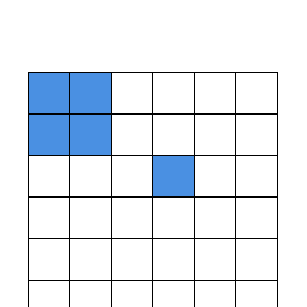
\begin{tikzpicture}[x=0.75pt,y=0.75pt,yscale=-1,xscale=1]
        %uncomment if require: \path (0,300); %set diagram left start at 0, and has height of 300
        
        %Shape: Grid [id:dp5859411922947491] 
        \draw  [draw opacity=0] (130,56.37) -- (250.26,56.37) -- (250.26,176.88) -- (130,176.88) -- cycle ; \draw   (130,56.37) -- (130,176.88)(150,56.37) -- (150,176.88)(170,56.37) -- (170,176.88)(190,56.37) -- (190,176.88)(210,56.37) -- (210,176.88)(230,56.37) -- (230,176.88)(250,56.37) -- (250,176.88) ; \draw   (130,56.37) -- (250.26,56.37)(130,76.37) -- (250.26,76.37)(130,96.37) -- (250.26,96.37)(130,116.37) -- (250.26,116.37)(130,136.37) -- (250.26,136.37)(130,156.37) -- (250.26,156.37)(130,176.37) -- (250.26,176.37) ; \draw    ;
        %Shape: Square [id:dp8831764696734834] 
        \draw  [fill={rgb, 255:red, 74; green, 144; blue, 226 }  ,fill opacity=1 ] (190,96.37) -- (210,96.37) -- (210,116.37) -- (190,116.37) -- cycle ;
        %Shape: Square [id:dp5537318101713737] 
        \draw  [fill={rgb, 255:red, 74; green, 144; blue, 226 }  ,fill opacity=1 ] (130,56.37) -- (150,56.37) -- (150,76.37) -- (130,76.37) -- cycle ;
        %Shape: Square [id:dp1925471334706612] 
        \draw  [fill={rgb, 255:red, 74; green, 144; blue, 226 }  ,fill opacity=1 ] (150,56.37) -- (170,56.37) -- (170,76.37) -- (150,76.37) -- cycle ;
        %Shape: Square [id:dp9750373039987941] 
        \draw  [fill={rgb, 255:red, 74; green, 144; blue, 226 }  ,fill opacity=1 ] (150,76.37) -- (170,76.37) -- (170,96.37) -- (150,96.37) -- cycle ;
        %Shape: Square [id:dp1124365862723069] 
        \draw  [fill={rgb, 255:red, 74; green, 144; blue, 226 }  ,fill opacity=1 ] (130,76.37) -- (150,76.37) -- (150,96.37) -- (130,96.37) -- cycle ;
        \end{tikzpicture}
        \]
\end{enumerate}

\textbf{Solution}: We'll solve the problem for distinct rooks labelled $1,2,\dots,6$ and then divide by $6!$. Let $S=$ all arrangements ignoring blue squares and $A_i=$ arrangements where rook $i$ is on a blue square.

We use symmetric IE:\sidenote{choose rows and choose columns} \begin{align*}
    \alpha_0 &= |S| = 6!\times 6!\\
    \alpha_1 &= |A_1| = \bt{5}\times (5!)^2\\
    \alpha_2 &= |A_1\cap A_2| = \bt{6}\cdot \rt{2!}\cdot (4!)^2
\end{align*}
\[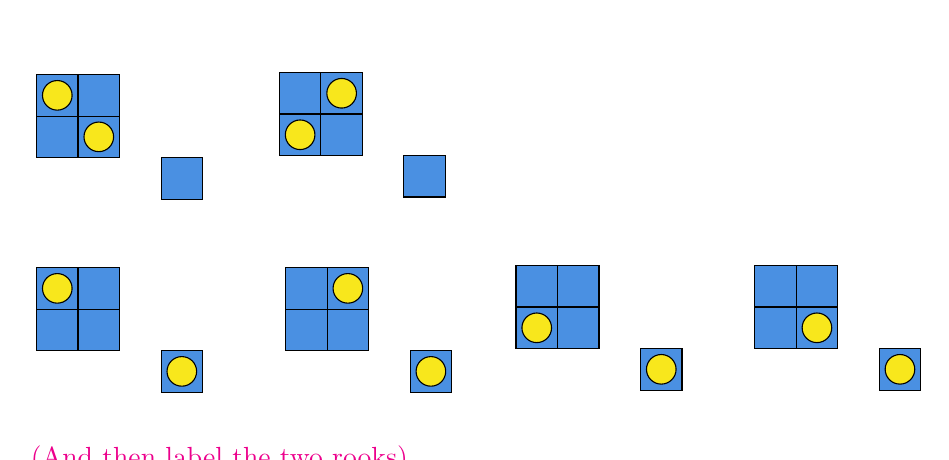
\begin{tikzpicture}[x=0.75pt,y=0.75pt,yscale=-1,xscale=1]
    %uncomment if require: \path (0,300); %set diagram left start at 0, and has height of 300
    
    %Shape: Square [id:dp8831764696734834] 
    \draw  [fill={rgb, 255:red, 74; green, 144; blue, 226 }  ,fill opacity=1 ] (115,85.37) -- (135,85.37) -- (135,105.37) -- (115,105.37) -- cycle ;
    %Shape: Square [id:dp5537318101713737] 
    \draw  [fill={rgb, 255:red, 74; green, 144; blue, 226 }  ,fill opacity=1 ] (55,45.37) -- (75,45.37) -- (75,65.37) -- (55,65.37) -- cycle ;
    %Shape: Square [id:dp1925471334706612] 
    \draw  [fill={rgb, 255:red, 74; green, 144; blue, 226 }  ,fill opacity=1 ] (75,45.37) -- (95,45.37) -- (95,65.37) -- (75,65.37) -- cycle ;
    %Shape: Square [id:dp9750373039987941] 
    \draw  [fill={rgb, 255:red, 74; green, 144; blue, 226 }  ,fill opacity=1 ] (75,65.37) -- (95,65.37) -- (95,85.37) -- (75,85.37) -- cycle ;
    %Shape: Square [id:dp1124365862723069] 
    \draw  [fill={rgb, 255:red, 74; green, 144; blue, 226 }  ,fill opacity=1 ] (55,65.37) -- (75,65.37) -- (75,85.37) -- (55,85.37) -- cycle ;
    %Shape: Circle [id:dp5567487821346038] 
    \draw  [fill={rgb, 255:red, 248; green, 231; blue, 28 }  ,fill opacity=1 ] (57.87,55.37) .. controls (57.87,51.43) and (61.06,48.24) .. (65,48.24) .. controls (68.94,48.24) and (72.13,51.43) .. (72.13,55.37) .. controls (72.13,59.31) and (68.94,62.5) .. (65,62.5) .. controls (61.06,62.5) and (57.87,59.31) .. (57.87,55.37) -- cycle ;
    %Shape: Circle [id:dp6716432582969902] 
    \draw  [fill={rgb, 255:red, 248; green, 231; blue, 28 }  ,fill opacity=1 ] (77.87,75.37) .. controls (77.87,71.43) and (81.06,68.24) .. (85,68.24) .. controls (88.94,68.24) and (92.13,71.43) .. (92.13,75.37) .. controls (92.13,79.31) and (88.94,82.5) .. (85,82.5) .. controls (81.06,82.5) and (77.87,79.31) .. (77.87,75.37) -- cycle ;
    %Shape: Square [id:dp4680473069566855] 
    \draw  [fill={rgb, 255:red, 74; green, 144; blue, 226 }  ,fill opacity=1 ] (232,84.37) -- (252,84.37) -- (252,104.37) -- (232,104.37) -- cycle ;
    %Shape: Square [id:dp14960112082385857] 
    \draw  [fill={rgb, 255:red, 74; green, 144; blue, 226 }  ,fill opacity=1 ] (172,44.37) -- (192,44.37) -- (192,64.37) -- (172,64.37) -- cycle ;
    %Shape: Square [id:dp428788690057446] 
    \draw  [fill={rgb, 255:red, 74; green, 144; blue, 226 }  ,fill opacity=1 ] (192,44.37) -- (212,44.37) -- (212,64.37) -- (192,64.37) -- cycle ;
    %Shape: Square [id:dp04451289815970538] 
    \draw  [fill={rgb, 255:red, 74; green, 144; blue, 226 }  ,fill opacity=1 ] (192,64.37) -- (212,64.37) -- (212,84.37) -- (192,84.37) -- cycle ;
    %Shape: Square [id:dp259419935190194] 
    \draw  [fill={rgb, 255:red, 74; green, 144; blue, 226 }  ,fill opacity=1 ] (172,64.37) -- (192,64.37) -- (192,84.37) -- (172,84.37) -- cycle ;
    %Shape: Circle [id:dp4647101461804377] 
    \draw  [fill={rgb, 255:red, 248; green, 231; blue, 28 }  ,fill opacity=1 ] (174.87,74.37) .. controls (174.87,70.43) and (178.06,67.24) .. (182,67.24) .. controls (185.94,67.24) and (189.13,70.43) .. (189.13,74.37) .. controls (189.13,78.31) and (185.94,81.5) .. (182,81.5) .. controls (178.06,81.5) and (174.87,78.31) .. (174.87,74.37) -- cycle ;
    %Shape: Circle [id:dp611186225390719] 
    \draw  [fill={rgb, 255:red, 248; green, 231; blue, 28 }  ,fill opacity=1 ] (194.87,54.37) .. controls (194.87,50.43) and (198.06,47.24) .. (202,47.24) .. controls (205.94,47.24) and (209.13,50.43) .. (209.13,54.37) .. controls (209.13,58.31) and (205.94,61.5) .. (202,61.5) .. controls (198.06,61.5) and (194.87,58.31) .. (194.87,54.37) -- cycle ;
    %Shape: Square [id:dp8903745605566249] 
    \draw  [fill={rgb, 255:red, 74; green, 144; blue, 226 }  ,fill opacity=1 ] (115,178.37) -- (135,178.37) -- (135,198.37) -- (115,198.37) -- cycle ;
    %Shape: Square [id:dp849694591772084] 
    \draw  [fill={rgb, 255:red, 74; green, 144; blue, 226 }  ,fill opacity=1 ] (55,138.37) -- (75,138.37) -- (75,158.37) -- (55,158.37) -- cycle ;
    %Shape: Square [id:dp04633393218424331] 
    \draw  [fill={rgb, 255:red, 74; green, 144; blue, 226 }  ,fill opacity=1 ] (75,138.37) -- (95,138.37) -- (95,158.37) -- (75,158.37) -- cycle ;
    %Shape: Square [id:dp8918671859575977] 
    \draw  [fill={rgb, 255:red, 74; green, 144; blue, 226 }  ,fill opacity=1 ] (75,158.37) -- (95,158.37) -- (95,178.37) -- (75,178.37) -- cycle ;
    %Shape: Square [id:dp5490922197293115] 
    \draw  [fill={rgb, 255:red, 74; green, 144; blue, 226 }  ,fill opacity=1 ] (55,158.37) -- (75,158.37) -- (75,178.37) -- (55,178.37) -- cycle ;
    %Shape: Circle [id:dp011688520313485773] 
    \draw  [fill={rgb, 255:red, 248; green, 231; blue, 28 }  ,fill opacity=1 ] (57.87,148.37) .. controls (57.87,144.43) and (61.06,141.24) .. (65,141.24) .. controls (68.94,141.24) and (72.13,144.43) .. (72.13,148.37) .. controls (72.13,152.31) and (68.94,155.5) .. (65,155.5) .. controls (61.06,155.5) and (57.87,152.31) .. (57.87,148.37) -- cycle ;
    %Shape: Circle [id:dp48423444740504906] 
    \draw  [fill={rgb, 255:red, 248; green, 231; blue, 28 }  ,fill opacity=1 ] (117.87,188.37) .. controls (117.87,184.43) and (121.06,181.24) .. (125,181.24) .. controls (128.94,181.24) and (132.13,184.43) .. (132.13,188.37) .. controls (132.13,192.31) and (128.94,195.5) .. (125,195.5) .. controls (121.06,195.5) and (117.87,192.31) .. (117.87,188.37) -- cycle ;
    %Shape: Square [id:dp42908952577197135] 
    \draw  [fill={rgb, 255:red, 74; green, 144; blue, 226 }  ,fill opacity=1 ] (235,178.37) -- (255,178.37) -- (255,198.37) -- (235,198.37) -- cycle ;
    %Shape: Square [id:dp2376698716530623] 
    \draw  [fill={rgb, 255:red, 74; green, 144; blue, 226 }  ,fill opacity=1 ] (175,138.37) -- (195,138.37) -- (195,158.37) -- (175,158.37) -- cycle ;
    %Shape: Square [id:dp44221223901669493] 
    \draw  [fill={rgb, 255:red, 74; green, 144; blue, 226 }  ,fill opacity=1 ] (195,138.37) -- (215,138.37) -- (215,158.37) -- (195,158.37) -- cycle ;
    %Shape: Square [id:dp07104162862528662] 
    \draw  [fill={rgb, 255:red, 74; green, 144; blue, 226 }  ,fill opacity=1 ] (195,158.37) -- (215,158.37) -- (215,178.37) -- (195,178.37) -- cycle ;
    %Shape: Square [id:dp206940095815624] 
    \draw  [fill={rgb, 255:red, 74; green, 144; blue, 226 }  ,fill opacity=1 ] (175,158.37) -- (195,158.37) -- (195,178.37) -- (175,178.37) -- cycle ;
    %Shape: Circle [id:dp5074157301280751] 
    \draw  [fill={rgb, 255:red, 248; green, 231; blue, 28 }  ,fill opacity=1 ] (197.87,148.37) .. controls (197.87,144.43) and (201.06,141.24) .. (205,141.24) .. controls (208.94,141.24) and (212.13,144.43) .. (212.13,148.37) .. controls (212.13,152.31) and (208.94,155.5) .. (205,155.5) .. controls (201.06,155.5) and (197.87,152.31) .. (197.87,148.37) -- cycle ;
    %Shape: Circle [id:dp842906997930893] 
    \draw  [fill={rgb, 255:red, 248; green, 231; blue, 28 }  ,fill opacity=1 ] (237.87,188.37) .. controls (237.87,184.43) and (241.06,181.24) .. (245,181.24) .. controls (248.94,181.24) and (252.13,184.43) .. (252.13,188.37) .. controls (252.13,192.31) and (248.94,195.5) .. (245,195.5) .. controls (241.06,195.5) and (237.87,192.31) .. (237.87,188.37) -- cycle ;
    %Shape: Square [id:dp3632936104650424] 
    \draw  [fill={rgb, 255:red, 74; green, 144; blue, 226 }  ,fill opacity=1 ] (346,177.37) -- (366,177.37) -- (366,197.37) -- (346,197.37) -- cycle ;
    %Shape: Square [id:dp8656436396921494] 
    \draw  [fill={rgb, 255:red, 74; green, 144; blue, 226 }  ,fill opacity=1 ] (286,137.37) -- (306,137.37) -- (306,157.37) -- (286,157.37) -- cycle ;
    %Shape: Square [id:dp3111030828407515] 
    \draw  [fill={rgb, 255:red, 74; green, 144; blue, 226 }  ,fill opacity=1 ] (306,137.37) -- (326,137.37) -- (326,157.37) -- (306,157.37) -- cycle ;
    %Shape: Square [id:dp49317680881038295] 
    \draw  [fill={rgb, 255:red, 74; green, 144; blue, 226 }  ,fill opacity=1 ] (306,157.37) -- (326,157.37) -- (326,177.37) -- (306,177.37) -- cycle ;
    %Shape: Square [id:dp659501862336836] 
    \draw  [fill={rgb, 255:red, 74; green, 144; blue, 226 }  ,fill opacity=1 ] (286,157.37) -- (306,157.37) -- (306,177.37) -- (286,177.37) -- cycle ;
    %Shape: Circle [id:dp8099820734048515] 
    \draw  [fill={rgb, 255:red, 248; green, 231; blue, 28 }  ,fill opacity=1 ] (288.87,167.37) .. controls (288.87,163.43) and (292.06,160.24) .. (296,160.24) .. controls (299.94,160.24) and (303.13,163.43) .. (303.13,167.37) .. controls (303.13,171.31) and (299.94,174.5) .. (296,174.5) .. controls (292.06,174.5) and (288.87,171.31) .. (288.87,167.37) -- cycle ;
    %Shape: Circle [id:dp4627082431613787] 
    \draw  [fill={rgb, 255:red, 248; green, 231; blue, 28 }  ,fill opacity=1 ] (348.87,187.37) .. controls (348.87,183.43) and (352.06,180.24) .. (356,180.24) .. controls (359.94,180.24) and (363.13,183.43) .. (363.13,187.37) .. controls (363.13,191.31) and (359.94,194.5) .. (356,194.5) .. controls (352.06,194.5) and (348.87,191.31) .. (348.87,187.37) -- cycle ;
    %Shape: Square [id:dp4889034753402557] 
    \draw  [fill={rgb, 255:red, 74; green, 144; blue, 226 }  ,fill opacity=1 ] (461,177.37) -- (481,177.37) -- (481,197.37) -- (461,197.37) -- cycle ;
    %Shape: Square [id:dp8539531217122311] 
    \draw  [fill={rgb, 255:red, 74; green, 144; blue, 226 }  ,fill opacity=1 ] (401,137.37) -- (421,137.37) -- (421,157.37) -- (401,157.37) -- cycle ;
    %Shape: Square [id:dp18832607171881954] 
    \draw  [fill={rgb, 255:red, 74; green, 144; blue, 226 }  ,fill opacity=1 ] (421,137.37) -- (441,137.37) -- (441,157.37) -- (421,157.37) -- cycle ;
    %Shape: Square [id:dp018087259514916187] 
    \draw  [fill={rgb, 255:red, 74; green, 144; blue, 226 }  ,fill opacity=1 ] (421,157.37) -- (441,157.37) -- (441,177.37) -- (421,177.37) -- cycle ;
    %Shape: Square [id:dp6676767610401377] 
    \draw  [fill={rgb, 255:red, 74; green, 144; blue, 226 }  ,fill opacity=1 ] (401,157.37) -- (421,157.37) -- (421,177.37) -- (401,177.37) -- cycle ;
    %Shape: Circle [id:dp9658612427583175] 
    \draw  [fill={rgb, 255:red, 248; green, 231; blue, 28 }  ,fill opacity=1 ] (423.87,167.37) .. controls (423.87,163.43) and (427.06,160.24) .. (431,160.24) .. controls (434.94,160.24) and (438.13,163.43) .. (438.13,167.37) .. controls (438.13,171.31) and (434.94,174.5) .. (431,174.5) .. controls (427.06,174.5) and (423.87,171.31) .. (423.87,167.37) -- cycle ;
    %Shape: Circle [id:dp9203997506720898] 
    \draw  [fill={rgb, 255:red, 248; green, 231; blue, 28 }  ,fill opacity=1 ] (463.87,187.37) .. controls (463.87,183.43) and (467.06,180.24) .. (471,180.24) .. controls (474.94,180.24) and (478.13,183.43) .. (478.13,187.37) .. controls (478.13,191.31) and (474.94,194.5) .. (471,194.5) .. controls (467.06,194.5) and (463.87,191.31) .. (463.87,187.37) -- cycle ;
    
    % Text Node
    \draw (51,223) node [anchor=north west][inner sep=0.75pt]   [align=left] {\rt{(And then label the two rooks)}};
    
    
    \end{tikzpicture}
    \]
    \begin{align*}
        \alpha_3 &= |A_1\cap A_2\cap A_3| = \bt{2}\cdot \rt{3!}\cdot (3!)^2
    \end{align*}
    \[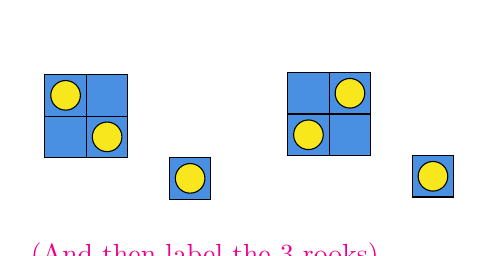
\begin{tikzpicture}[x=0.75pt,y=0.75pt,yscale=-1,xscale=1]
        %uncomment if require: \path (0,300); %set diagram left start at 0, and has height of 300
        
        %Shape: Square [id:dp7647996785236888] 
        \draw  [fill={rgb, 255:red, 74; green, 144; blue, 226 }  ,fill opacity=1 ] (115,85.37) -- (135,85.37) -- (135,105.37) -- (115,105.37) -- cycle ;
        %Shape: Square [id:dp015685356939575845] 
        \draw  [fill={rgb, 255:red, 74; green, 144; blue, 226 }  ,fill opacity=1 ] (55,45.37) -- (75,45.37) -- (75,65.37) -- (55,65.37) -- cycle ;
        %Shape: Square [id:dp43847879373489773] 
        \draw  [fill={rgb, 255:red, 74; green, 144; blue, 226 }  ,fill opacity=1 ] (75,45.37) -- (95,45.37) -- (95,65.37) -- (75,65.37) -- cycle ;
        %Shape: Square [id:dp6228251360346071] 
        \draw  [fill={rgb, 255:red, 74; green, 144; blue, 226 }  ,fill opacity=1 ] (75,65.37) -- (95,65.37) -- (95,85.37) -- (75,85.37) -- cycle ;
        %Shape: Square [id:dp38618928842407807] 
        \draw  [fill={rgb, 255:red, 74; green, 144; blue, 226 }  ,fill opacity=1 ] (55,65.37) -- (75,65.37) -- (75,85.37) -- (55,85.37) -- cycle ;
        %Shape: Circle [id:dp29543074502201283] 
        \draw  [fill={rgb, 255:red, 248; green, 231; blue, 28 }  ,fill opacity=1 ] (57.87,55.37) .. controls (57.87,51.43) and (61.06,48.24) .. (65,48.24) .. controls (68.94,48.24) and (72.13,51.43) .. (72.13,55.37) .. controls (72.13,59.31) and (68.94,62.5) .. (65,62.5) .. controls (61.06,62.5) and (57.87,59.31) .. (57.87,55.37) -- cycle ;
        %Shape: Circle [id:dp05505992816398875] 
        \draw  [fill={rgb, 255:red, 248; green, 231; blue, 28 }  ,fill opacity=1 ] (77.87,75.37) .. controls (77.87,71.43) and (81.06,68.24) .. (85,68.24) .. controls (88.94,68.24) and (92.13,71.43) .. (92.13,75.37) .. controls (92.13,79.31) and (88.94,82.5) .. (85,82.5) .. controls (81.06,82.5) and (77.87,79.31) .. (77.87,75.37) -- cycle ;
        %Shape: Square [id:dp47440460175044663] 
        \draw  [fill={rgb, 255:red, 74; green, 144; blue, 226 }  ,fill opacity=1 ] (232,84.37) -- (252,84.37) -- (252,104.37) -- (232,104.37) -- cycle ;
        %Shape: Square [id:dp976583308270353] 
        \draw  [fill={rgb, 255:red, 74; green, 144; blue, 226 }  ,fill opacity=1 ] (172,44.37) -- (192,44.37) -- (192,64.37) -- (172,64.37) -- cycle ;
        %Shape: Square [id:dp12942166734557947] 
        \draw  [fill={rgb, 255:red, 74; green, 144; blue, 226 }  ,fill opacity=1 ] (192,44.37) -- (212,44.37) -- (212,64.37) -- (192,64.37) -- cycle ;
        %Shape: Square [id:dp09091446381146073] 
        \draw  [fill={rgb, 255:red, 74; green, 144; blue, 226 }  ,fill opacity=1 ] (192,64.37) -- (212,64.37) -- (212,84.37) -- (192,84.37) -- cycle ;
        %Shape: Square [id:dp8035752753802121] 
        \draw  [fill={rgb, 255:red, 74; green, 144; blue, 226 }  ,fill opacity=1 ] (172,64.37) -- (192,64.37) -- (192,84.37) -- (172,84.37) -- cycle ;
        %Shape: Circle [id:dp26388211245030435] 
        \draw  [fill={rgb, 255:red, 248; green, 231; blue, 28 }  ,fill opacity=1 ] (174.87,74.37) .. controls (174.87,70.43) and (178.06,67.24) .. (182,67.24) .. controls (185.94,67.24) and (189.13,70.43) .. (189.13,74.37) .. controls (189.13,78.31) and (185.94,81.5) .. (182,81.5) .. controls (178.06,81.5) and (174.87,78.31) .. (174.87,74.37) -- cycle ;
        %Shape: Circle [id:dp009695476041065465] 
        \draw  [fill={rgb, 255:red, 248; green, 231; blue, 28 }  ,fill opacity=1 ] (194.87,54.37) .. controls (194.87,50.43) and (198.06,47.24) .. (202,47.24) .. controls (205.94,47.24) and (209.13,50.43) .. (209.13,54.37) .. controls (209.13,58.31) and (205.94,61.5) .. (202,61.5) .. controls (198.06,61.5) and (194.87,58.31) .. (194.87,54.37) -- cycle ;
        %Shape: Circle [id:dp49805507666280247] 
        \draw  [fill={rgb, 255:red, 248; green, 231; blue, 28 }  ,fill opacity=1 ] (117.87,95.37) .. controls (117.87,91.43) and (121.06,88.24) .. (125,88.24) .. controls (128.94,88.24) and (132.13,91.43) .. (132.13,95.37) .. controls (132.13,99.31) and (128.94,102.5) .. (125,102.5) .. controls (121.06,102.5) and (117.87,99.31) .. (117.87,95.37) -- cycle ;
        %Shape: Circle [id:dp09557794098498462] 
        \draw  [fill={rgb, 255:red, 248; green, 231; blue, 28 }  ,fill opacity=1 ] (234.87,94.37) .. controls (234.87,90.43) and (238.06,87.24) .. (242,87.24) .. controls (245.94,87.24) and (249.13,90.43) .. (249.13,94.37) .. controls (249.13,98.31) and (245.94,101.5) .. (242,101.5) .. controls (238.06,101.5) and (234.87,98.31) .. (234.87,94.37) -- cycle ;
        
        % Text Node
        \draw (47,125) node [anchor=north west][inner sep=0.75pt]   [align=left] {\rt{(And then label the 3 rooks)}};
        
        
        \end{tikzpicture}
        \]
        \begin{align*}
            \alpha_4=\alpha_5=\alpha_6=0
        \end{align*}

Hence, by symmetric IE, the answer for labelled rooks would be: \begin{align*}
    &(6!)^2-\pt{6\choose 1}\cdot \bt{5}\cdot \rt 1!\cdot (5!)^2 + \pt{6\choose 2}\cdot \bt{6}\cdot \rt{2!}\cdot (4!)^2 -\pt{6\choose 3}\cdot \bt{2}\cdot \rt{3!}\cdot (3!)^2\\
    =& 6!6! - \pt{\frac{6!}{1!5!}}\cdot \bt{5}\cdot \rt{1}\cdot5!5!+\pt{\frac{6!}{2!4!}}\cdot\bt{6}\cdot\rt{2!}\cdot4!4! - \pt{\frac{6!}{3!3!}}\cdot\bt{2}\cdot \rt{3!}3!3!\\
    =& 6!(6!-\bt{5}\cdot5!+\bt{6}\cdot4!-\bt{2}\cdot3!)
\end{align*}
Therefore, the \textbf{unlabelled} rooks have an answer of $6!-\bt{5}\cdot5!+\bt{6}\cdot4!-\bt{2}\cdot3!=252$.

\subsubsection{General rook formula}
The number of ways to place $n$ rooks on a $n\times n$ board such that \begin{enumerate}
    \item no two in the same row or column
    \item no rook on blue squares\end{enumerate}
is \[n!-\bt{r_1}(n-1)!+\dots+(-1)^n\bt{r_n}0!\] where $\bt{r_k}$ is the number of ways to place $k$ identical rooks on blue squares satisfying rule 1.

\section{H Power series}
\subsection{H1 Geometric series}
Let $$\begin{matrix}
    S &= 1+&x+x^2+\dots + x^n\\
    xS &= &x+x^2+\dots + x^n +x^{n+1}
\end{matrix}$$
Hence, \rt{$1+x+\dots+x^n = \frac{1-x^{n+1}}{1-x}$} whenever $x\neq 1$. If $x=1$, then the sum is simply $n+1$.\sidenote{Works in any division ring!}

\rmk A variation: 
\tbd{Do notes from 3/25 and 3/27}

\begin{theorem}
    It is impossible to tile a $10\times 10$ square using $1\times 4$ tiles.
\end{theorem}

\subsection{H3 9899\textsuperscript{-1}}
Mystery: \[\frac{1}{9899}=0.00\,01\,01\,02\,03\,05\dots\]

Explanation: If we have $f_0=0, f_1=1$ and $f_n=f_{n-1}+f_{n-2}$, then the RHS looks like \[\sum_{k=0}^{\infty}\frac{f_k}{100^{k+1}}=\frac{1}{100}\sum_{k=0}^{\infty}f_k\left(\frac{1}{100}\right)^k\]
Consider \(F(x)=\sum_{k=0}^{\infty}f_kx^k\). The series converges for $|x|<\frac{1}{2}$ because we can easily bound it above through $f_k\leq 2^k$\sidenote{There exists a better bound, but this is sufficient.} by induction. Hence, we observe:\[\begin{array}{rlll}
    F &= 0+x+ & x^2+  & 2x^3+\dots +f_nx^n+\dots \\
    xF &= & x^2+ & x^3+\dots +f_{n-1}x^n+\dots\\
    x^2F &= & & x^3+\dots +f_{n-2}x^n+\dots\\ \hline
    F-xF-x^2F &= 0+x + & 0x^2 + &\dots
    \end{array}
    \]
Therefore, we have a closed form for $f_n$: \[\sum f_n x^n = \frac{x}{1-x-x^2}\]
Therefore, the RHS could be written as: \begin{align*}
    0.0001010203\dots &= \frac{1}{100}\sum f_n\left(\frac{1}{100}\right)^n\\
    &= \frac{1}{100}\cdot \frac{\frac{1}{100}}{1-\frac{1}{100}-\frac{1}{100^2}}\\
    &= \frac{1}{9899}\\
    &= LHS
\end{align*}\qed

\subsubsection{More on the closed form of $f_n$}
Write $1-x-x^2=(x-\alpha)(x-\beta)$. 
Therefore, $\alpha,\beta=-\frac{1\pm \sqrt{5}}{2}$. We then use partial fractions to get \begin{align*}
    \sum f_nx^n &=\frac{x}{1-x-x^2}\\
    &= \frac{-\alpha}{\alpha-\beta}\cdot \frac{1}{x-\alpha}+\frac{\beta}{\alpha-\beta}\cdot \frac{1}{x-\beta}\\
    &= \frac{-1}{\alpha-\beta}\left(\frac{1}{\frac{x}{\alpha}-1}-\frac{1}{\frac{x}{\beta}-1}\right)\\
    &= \frac{1}{\alpha-\beta}\left(\frac{1}{1-\frac{x}{\alpha}}-\frac{1}{1-\frac{x}{\beta}}\right)\qquad \text{by geometric series formula,}\\
    &= \frac{1}{\alpha-\beta}\left(\sum_{i=0}^{\infty}\left(\frac{x}{\alpha}\right)^i-\sum_{i=0}^{\infty}\left(\frac{x}{\beta}\right)^i\right)
\end{align*}
Hence, we get the constant term of the $n$-th derivative:
	\begin{align*}
		\frac{f^{(n)}(0)}{n!} &= \frac{1}{\alpha-\beta}\cdot \left(n!\frac{1}{\alpha^n}-n!\frac{1}{\beta^n}\right)\cdot \frac{1}{n!}\\
		&= \frac{1}{\alpha-\beta}\cdot \left(\frac{1}{\alpha^n}-\frac{1}{\beta^n}\right)\\
		&=\frac{1}{\sqrt{5}}\left(\frac{1}{\beta^n}-\frac{1}{\alpha^n}\right)
	\end{align*}
	Since $\alpha=\frac{-(1+\sqrt{5})}{2}, \beta=\frac{-(1-\sqrt{5})}{2}$, we observe that $\frac{1}{\alpha}=\frac{1-\sqrt{5}}{2}$ and $\frac{1}{\beta}=\frac{1+\sqrt{5}}{2}$. Thus, we substitute them back in:
	\begin{align*}
		\frac{f^{(n)}(0)}{n!} &= \frac{1}{\sqrt{5}}\left(\frac{1}{\beta^n}-\frac{1}{\alpha^n}\right)\\
		&=\frac{1}{\sqrt{5}} \bigg( \bigg( \frac{1 + \sqrt{5}}{2}\bigg)^n - \bigg( \frac{1 - \sqrt{5}}{2}\bigg)^n \bigg)
	\end{align*}
	which is Binet's formula.

\begin{theorem}[Binet's formula]
    $\displaystyle
				f_n = \frac{1}{\sqrt{5}} \bigg( \bigg( \frac{1 + \sqrt{5}}{2}\bigg)^n - \bigg( \frac{1 - \sqrt{5}}{2}\bigg)^n \bigg)$
\end{theorem}

\begin{corollary}
    $\displaystyle
				f_n \to \frac{1}{\sqrt{5}} \bigg( \frac{1 + \sqrt{5}}{2}\bigg)^n$ as $n\to \infty$.
\end{corollary}

\tbd{Type the $\sigma$ example}
\subsection{H4 Polynomial power series}

We were able to obtain a formula for the Fibonacci numbers \[0,1,1,2,3,5,8,\dots\]
by converting the sequence into a function \[F(x)=\sum_{n=0}^{\infty}f_nx^n\]
We showed that \[F(x)=\frac{x}{1-x-x^2} = \frac{A}{1-\alpha x}+\frac{B}{1-\beta x}\]
and we used the geometric series \[\frac{1}{1-\alpha x}=\sum_{n=0}^{\infty}(\alpha x)^n\]
to get \[f_n=A\alpha^n +B\beta^n\]
\spl

In general, partial fractions will involve terms of the form \[\frac{1}{1-\alpha x},\frac{1}{(1-\alpha x)^2},\frac{1}{(1-\alpha x)^3},\dots\]

\begin{theorem}
    \[\frac{1}{(1-x)^k}=\sum_{n=0}^{\infty}\left({k\choose n}\right)x^n\]
    valid when $|x|<1$. \sidenote{\(\left({k\choose n}\right) = {k+n-1\choose n}\)}
    It follows that:
    \[\frac{1}{(1-\alpha x)^k}=\sum_{n=0}^{\infty}\left({k\choose n}\right)\alpha^nx^n\] when \(|x|<\left|\frac{1}{\alpha}\right|\).
\end{theorem}

\begin{proof}
    We observe that when the geometric sequence converges absolutely: \begin{align*}
        LHS &= (1+x+x^2+\dots)^k\\
        &= \underset{k}{\underbrace{(1+x+x^2+\dots)\cdot (1+x+x^2+\dots)\cdot \dots \cdot (1+x+x^2+\dots)}}
    \end{align*}
    To get the coefficient for $x^n$, we want to select terms from each bracket \[x^{a_1},x^{a_2},\dots,x^{a_k}\]
    such that $a_1+a_2+\dots+a_k=n$. This is equivalent to the problem of choosing a bag of $n$ bagels of $k$ different types.
\end{proof}

\spl

Last time, we found a formula \[\sum_{n=0}^{\infty}n^2x^n = \frac{x+x^2}{(1-x)^3}\] using derivatives.

We now have an alternative approach:
\begin{align*}
    \mchoose{1}{n} &= {n+0\choose 0}=1\\
    \mchoose{2}{n} &= {n+1\choose 1}=n+1\\
    \mchoose{3}{n} &= {n+2\choose 2} = \frac{(n+2)(n+1)}{2}
\end{align*}
Write $n^2$ as a linear combination of them:\[n^2 = \rt{2}\cdot \frac{(n+2)(n+1)}{2} \rt{-3}(n+1)+\rt{1}\cdot1\]
And so \begin{align*}
    \sum_{n=0}^{\infty}n^2x^n &= \sum_{n=0}^{\infty}\left(\rt{2}\cdot \frac{(n+2)(n+1)}{2} -\rt{3}(n+1)+\rt{1}\cdot1\right)x^n\\
    &= \frac{\rt{2}}{(1-x)^3}+\frac{\rt{-3}}{(1-x)^2}+\frac{\rt{1}}{1-x}\\
    &= \frac{x^2+x}{(1-x)^3}
\end{align*}

\rmk We have two natural bases for the vector space of polynomials in $n$:\[\begin{matrix}
    1,&n,&n^2,&n^3,\dots\\
    \mchoose{1}{n},&\mchoose{2}{n},&\mchoose{3}{n},&\mchoose{4}{n},\dots
\end{matrix}\]

\subsection{H5 Linear recurrence relations}
We can apply our analysis of the Fibonacci series $f_0=0,f_1=1,f_n=f_{n-1}+f_{n-2}$ to more general recursively-defined sequences.

\subsubsection{Homogeneous order-$k$ linear recurrence}
\[g_n=c_{1}g_{n-1} + c_{2}g_{n-2} +\dots + c_{k}g_{n-k}\]
with $n\geq k$ and initial conditions $g_0=a_0, g_1=a_1,\dots, g_{k-1}=a_{k-1}$.

\eg Order 2 with distinct roots: \[\begin{cases}
    g_n = 2g_{n-1}+3g_{n-2}\\
    g_0=3,g_1=5
\end{cases}\]
And so $(g_n)=(3,5,19,53,163,\dots)$.

Let $G(x)=\sum_{n=0}^{\infty}g_nx^n$.
\[\begin{array}{rlll}
    G &= 3+&5x+ & 19x^2+   \dots +g_nx^n+\dots \\
    xG &= &3x+& 5x^2+\dots +g_{n-1}x^n+\dots\\
    x^2G &= && 3x^2 + \dots +g_{n-2}x^n+\dots\\ \hline
    G-2xG-3x^2G &= 3-&x + & 0x^2 + \dots
    \end{array}
    \]
And hence $(1-2x-3x^2)G=3-x$. Therefore, \begin{align*}
    G= \frac{3-x}{1-2x-3x^2} &= \frac{3-x}{(1-3x)(1+x)}\\
    &= \frac{2}{1-3x}+\frac{1}{1+x}\\
    &= \sum_{n=0}^{\infty}(2\cdot 3^n + 1\cdot(-1)^n)x^n
\end{align*}
And so $g_n=2\cdot 3^n + (-1)^n$.

\eg Order 2 with repeated roots:
\[\begin{cases}
    g_n = 4g_{n-1}+4g_{n-2}\\
    g_0=1,g_1=6
\end{cases}\]
Thus, the sequence is $(g_n)=(1,6,20,56,144\dots)$.

Let $G(x)=\sum_{n=0}^{\infty}g_nx^n$.
\[\begin{array}{rlll}
    G &= 1+&6x+ & 20x^2+   \dots +g_nx^n+\dots \\
    xG &= &x+& 6x^2+\dots +g_{n-1}x^n+\dots\\
    x^2G &= && x^2 + \dots +g_{n-2}x^n+\dots\\ \hline
    G-4xG-4x^2G &=1+&2x + & 0x^2 + \dots
    \end{array}
    \]
    And hence $(1-4x-4x^2)G=1+2x$. Therefore, \begin{align*}
        G= \frac{1+2x}{1-4x-4x^2} &= \frac{1+2x}{(1-2x)^2}\\
        &= \frac{2}{(1-2x)^2}+\frac{-1}{1-2x}\\
        &= \sum_{n=0}^{\infty}(2\cdot \mchoose{2}{n}2^n +(-1)2^n)x^n
    \end{align*}
We observe $\mchoose{2}{n} = n+1$, so $g_n=2^n(2n+1)$.

\subsubsection{Inhomogeneous recurrence}
Inhomogeneous: there are some other known sequences added.
\eg Inhomogeneous, order 1:\[\begin{cases}
    g_n=-g_{n-1}+2^n\\
    g_0=1
\end{cases}\]
Then $(g_n)=(1,1,3,5,11,\dots)$.

Let $G =\sum_{n=0}^{\infty}g_nx^n$ and observe that $H= \sum_{n=0}^{\infty}2^nx^n=\frac{1}{1-2x}$.
\[\begin{array}{rlll}
    G &= 1+&x+ & 3x^2+   \dots +g_nx^n+\dots \\
    xG &= &x+& x^2+\dots +g_{n-1}x^n+\dots\\
    H &= 1 + &2x & 4x^2 + \dots +g_{n-2}x^n+\dots\\ \hline
    G+xG-H &=1+&2x + & 4x^2 + 0 + \dots
    \end{array}
 \]
Thus, $G=\frac{1}{(1+x)(1-2x)}=\frac{2/3}{1-2x}+\frac{1/3}{1+x} = \sum_{n=0}^{\infty}(\frac{2}{3}\cdot 2^n +\frac{1}{3}(-1)^n)$. Hence, $g_n = \frac{2^{n+1}+(-1)^n}{3}$.

\subsection{H6 Nickels and dimes}
\eg \label[example]{nickels-only} How many ways are there to make \$1.03 out of nickels (5¢) and pennies (1¢)?

Answer: that would be the number of solutions to $5a+b=103$ with $a,b\in \N$. We can have: \[(a,b)=(0,103),(1,98),\dots,(20,3)\]

More generally, the number of solutions to $5a+b=n$ is $\lfloor \frac{n}{5}\rfloor + 1$ since the number of nickels have to be $a=0,1,\dots,\lfloor\frac{n}{5}\rfloor$.

\eg \label[example]{nickels-dime} How many ways are there to make \$1.03 out of dimes (10¢), nickels (5¢) and pennies (1¢)?

We use the previous solution: \begin{itemize}
    \item 0 dimes: $\lfloor\frac{103}{5}\rfloor + 1 = 21$
    \item 1 dimes: $\lfloor\frac{93}{5}\rfloor + 1 = 19$
    \item \dots
    \item 10 dimes: $\lfloor\frac{3}{5}\rfloor + 1 = 1$
\end{itemize}
Then we sum them up. Since they are consecutive odd numbers, \[21+19+17+\dots+1=11^2=121\]

\subsubsection{Another method}
Revisit \cref{nickels-only}. 

Consider the rational function \[\frac{1}{1-x}\cdot \frac{1}{1-x^5}= (1+x+x^2+x^3+\dots)(1+x^5+x^{10}+x^{15}+\dots)\]
we want to know what the coefficient for $x^{103}$ is. Note this is equivalent to the previous example since we are choosing $x^p$ terms from the first part and $x^{5q}$ terms from the second part, and we are looking for ways to get $5q+p=103$.

To get the coefficient of $x^{103}$, consider \[1+x+x^2+x^3+x^4 = \frac{1-x^5}{1-x}\]

And hence $\frac{1}{1-x}=\frac{1+x+x^2+x^3+x^4}{1-x^5}$. Furthermore, we see that \[\frac{1}{(1-x^5)^2}=\sum_{n\geq 0}\mchoose{2}{n}(x^5)^n\] We observe that the LHS becomes: \begin{align*}
    \frac{1}{1-x}\cdot \frac{1}{1-x^5} &= \frac{1+x+x^2+x^3+x^4}{1-x^5}\cdot \frac{1}{1-x^5}\\
    &= (\rt{1+x+x^2+x^3+x^4})\cdot \bt{\sum_{n\geq 0}\mchoose{2}{n}(x^5)^n}
\end{align*}
To get $x^{103}$, we want $x^p \cdot x^{5q}=x^{103}$ such that $0\leq p\leq 4$ and $q\geq 0$. The only solution is $(p,q)=(3,20)$. The coefficient is therefore \[\rt{1}\cdot \bt{\mchoose{2}{20}}=21\]

Now revisit \cref{nickels-dime}
Similarly, consider \[\frac{1}{1-x}\cdot \frac{1}{1-x^5}\cdot \frac{1}{1-x^{10}}= (1+x+x^2+x^3+\dots)(1+x^5+x^{10}+x^{15}+\dots)(1+x^{10}+x^{20}+\dots)\]
We now want to get the coefficient of $x^{103}$, which are from choosing terms $x^{a}, x^{5b}$, and $x^{10c}$ from the parts above such that $a+5b+10c=103$.

Also, we prepare that \[\frac{1}{1-x}=\frac{1+x+x^2+x^3+\dots+x^9}{1-x^{10}}\] and \[\frac{1}{1-x^5}=\frac{1+x^5}{1-x^{10}}\]
We observe that the LHS becomes:
\begin{align*}
    &\frac{1}{1-x}\cdot \frac{1}{1-x^5}\cdot \frac{1}{1-x^{10}}\\
    =& \frac{1+x+x^2+x^3+\dots+x^9}{1-x^{10}}\cdot \frac{1+x^5}{1-x^{10}} + \frac{1}{1-x^{10}}\\
    =& \rt{(1+x+\dots + x^4 + 2(x^5+\dots+x^9)+x^{10}+\dots + x^{14})} \cdot \bt{\sum_{n\geq 0}\mchoose{3}{n}x^{10}}
\end{align*}
We pick an $\rt{x^p}$ term from the first part and a $\bt{x^{10q}}$ term from the 2nd part such that $p+10q=103$, $0\leq p\leq 14$ and $q\geq 0$. 

There are two solutions: $(p,q)=(3,10)$ or $(13,9)$. The coefficient of $x^{103}$ is $$1\cdot \mchoose{3}{10}+1\cdot \mchoose{3}{9}=66+55=121$$

\subsection{H7 Characteristic ops and egf}\hypertarget{characteristic-ops-egf}{}
\cref{nickels-only} and \cref{nickels-dime} are equivalent to asking \textit{How many ways to get a bag of 103 bagels}:
\begin{enumerate}
    \item of 2 types, plain + garlic such that we can get any number of plain but garlic must be a multiple of 5?
    \item of 3 types, plain + garlic + onion, where can get any number of plain, but garlic must be a multiple of 5 and onion has to be a multiple of 10?
\end{enumerate}

These are combinations with constraints. That is, we want to put 103 ``balls'' in buckets \[U_{p}, U_{g}, U_{o}\] with capacities \begin{align*}
    U_p&\in \{0,1,2,\dots\} = N_p\\
    U_g&\in \{0,5,10,\dots\}= N_g\\
    U_o&\in \{0,10,20,\dots\}= N_0\\
\end{align*}
Effectively, we convert each set to a power series. There are two ways to convert a subset $N\subseteq\N$ into a power series. \begin{itemize}
    \item Step 1: Convert $N$ into a 0-1 sequence: \[a=(a_n) \text{ where }a_n=\begin{cases}
        1 & \text{if }n\in N\\
        0 & \text{ otherwise}
    \end{cases}\]
    \item Step 2: \begin{itemize}
        \item Characteristic OPS (ordinary power series) $X_N$ of $N$: \[(a_n)\mapsto \sum_{n\geq 0 }a_nx^n\]
        \item Characteristic EGF (exponential generating function) $\mathfrak{X}_n$ of $N$: \[(a_n)\mapsto \sum_{n\geq 0}\frac{a_n}{n!}x^n\]
    \end{itemize}
\end{itemize}

\eg $N=\{0,1,2,\dots\}$ \hfill(no constraint)\begin{align*}
    a^N &= 1,1,1,\dots\\
    X_N &= 1+x+x^2 +\dots = \frac{1}{1-x}\\
    \mathfrak{X}_N &= 1+x+\frac{x^2}{2!}+\dots = e^x
\end{align*}

\eg $N=\{1,2,3,\dots\}$ \hfill(at least 1 object)\begin{align*}
    a^N &= 0,1,1,\dots\\
    X_N &= x+x^2 +\dots = \frac{x}{1-x}\\
    \mathfrak{X}_N &= x+\frac{x^2}{2!}+\dots = e^x-1
\end{align*}

\eg $N=\{0,1\}$ \hfill(at most 1 object)\begin{align*}
    a^N &= 1,1,0,0,\dots\\
    X_N &= 1+x\\
    \mathfrak{X}_N &= 1+x
\end{align*}

\eg $N=\{0,2,4,6,\dots\}$ \hfill(even numbers of object)\begin{align*}
    a^N &= 1,0,1,0,\dots\\
    X_N &= 1+x^2 +x^4+\dots = \frac{x}{1-x^2}\\
    \mathfrak{X}_N &= 1+\frac{x^2}{2!}+\frac{x^4}{4!}+\dots = \cosh x = \frac{e^x+e^{-x}}{2}
\end{align*}

\eg $N=\{1,3,5,7,\dots\}$ \hfill(odd numbers of object)\begin{align*}
    a^N &= 0,1,0,1,\dots\\
    X_N &= x+x^3 +x^5+\dots = \frac{x}{1-x^2}\\
    \mathfrak{X}_N &= x+\frac{x^3}{3!}+\frac{x^5}{5!}+\dots = \sinh x = \frac{e^x-e^{-x}}{2}
\end{align*}

\eg $N=\{0,5,10,15,\dots\}$ \hfill(multiples of 5 numbers of object)\begin{align*}
    a^N &= 1,0,0,0,0,1,0,\dots\\
    X_N &= 1+x^5 +x^10+\dots = \frac{1}{1-x^5}\\
    \mathfrak{X}_N &= 1+\frac{x^5}{5!}+\frac{x^{10}}{10!}+\dots = \frac{1}{5}\sum_{k=0}^{4}e^{\omega^k x}
\end{align*}
where $\omega=e^{2\pi i/5}$ is a primitive 5th root of unity.

\section{I Generating functions}
\subsection{I1 OPS and EGF}
Suppose a combiatorial problem has an answer $a_n$ for each $n\geq 0$. We will encode an entire sequence $(a_n)$ as a function and try to find the function.

\defn[Ordinary power series] \[g(x)=\sum_n a_nx^n\]

\defn[Exponential generating function]\[G(x)=\sum_n \frac{a_n}{n!}x^n\]

\rmk Special case mentioned \hyperlink{characteristic-ops-egf}{here}: if $(a_n)$ is a sequence of 0s and 1s where $a_n=\begin{cases}
    1 & n\in N\\
    0 & n\notin N
\end{cases}$ for some set $N\subseteq\N$, then $g=X_n$ and $G=\mathfrak{X}_n$.

% \rmk Notes: \tbd{}

\eg Sequence: $1,1,1,1,\dots$
\begin{itemize}
    \item OPS: $1+x+x^2+\dots=\frac{1}{1-x}$\sidenote{$|x|<1$}
    \item EGF: $1+x+\frac{x^2}{2!}+\dots = e^x$
\end{itemize}

\eg Sequence: $1,\alpha,\alpha^2,\dots$
\begin{itemize}
    \item OPS: $1+\alpha x+\alpha x^2+\dots=\frac{1}{1-\alpha x}$\sidenote{$|x|<1/|\alpha|$}
    \item EGF: $1+\alpha x+\frac{\alpha^2x^2}{2!}+\dots = e^{\alpha }$
\end{itemize}

\eg Sequence: $a_n={m\choose n}$ \[{m\choose 0}, {m\choose 1}, \dots, {m\choose m}, 0,0,0,\dots\]
\begin{itemize}
    \item OPS: ${m\choose 0}+ {m\choose 1}x+ \dots+ {m\choose m}x^m =(1+x)^m$
    \item EGF: ${m\choose 0}+ {m\choose 1}x+{m\choose 2}\frac{x^2}{2!}+ \dots+{m\choose m}\frac{x^m}{m!}=??$\sidenote{We don't know how to solve this yet!}
\end{itemize}

\eg Sequence: $a_n=(m)_n$ \[(m)_0,(m)_1,\dots, (m)_m, 0,0,0,\dots\]
\begin{itemize}
    \item OPS: $(m)_0+(m)_1x+\dots+(m)_mx^m=??$\sidenote{We don't know how to solve this yet!}
    \item EGF: $(m)_0+(m)_1x+\frac{(m)_2}{2!}x^2+\dots +\frac{(m)_m}{m!}x^m = (1+x)^m$\sidenote{Since $\frac{(m)_k}{k!}={m\choose k}$}
\end{itemize}

\rmk Two skills needed: \begin{enumerate}
    \item Recognizing OPS/EGF as a function
    \item Given OPS/EGF, finding sequence $(a_n)$.
\end{enumerate}

\defn Notation: Write $[x^n:g]= x^n$ coefficient of the Taylor series of function $g$.

\rmk If $(a_n)\xrightarrow{ops} g(x)$, then $a_n=[x^n:g]$. Similarly, if $(a_n)\xrightarrow{egf}G(x)$, then $a_n=n![x^n:G]$. 

\subsection{I2 The multiplication rule}
\begin{proposition} \label[proposition]{ops-mult-rule}
    Suppose $$\begin{aligned}
    (a_n)&\xrightarrow{ops}f\\
    (b_n)&\xrightarrow{ops}g
\end{aligned}$$ Let $f\circ g\xleftarrow{ops}(c_n)$. Then \[c_n=\sum_{k=0}^{n}a_kb_{n-k}\]
\end{proposition}

\begin{proof}
    Make a multiplication table.
    \tbd{}
\end{proof}

\begin{proposition}
    Suppose $$\begin{aligned}
        (a_n)&\xrightarrow{egf}F\\
        (b_n)&\xrightarrow{egf}G
    \end{aligned}$$ Let $F\circ G\xleftarrow{egf}(c_n)$. Then \[c_n=\sum_{k=0}^{n}{n\choose k}a_kb_{n-k}\]
\end{proposition}
\begin{proof}
    We observe \begin{align*}
        (a_n)\xrightarrow{egf}&F\xleftarrow{ops}\left(\frac{a_n}{n!}\right)\\
        (b_n)\xrightarrow{egf}&G\xleftarrow{ops}\left(\frac{b_n}{n!}\right)\\
        (c_n)\xrightarrow{egf}&F\circ G\xleftarrow{ops}\left(\frac{c_n}{n!}\right)\\
    \end{align*}
    By \cref{ops-mult-rule}, we get \[\frac{c_n}{n!}=\sum_{k=0}^{n}\left(\frac{a_k}{k!}\right)\left(\frac{b_{n-k}}{(n-k)!}\right)\]
    Therefore, $\displaystyle c_n=\sum_{k=0}^{n}{n\choose k}a_kb_{n-k}$.
\end{proof}

\begin{proposition}[Generalization]
    Sequences \[\begin{tikzcd}[ampersand replacement=\&,cramped]
        {(a_n^1),(a_n^2),\dots,(a_n^t)} \\
        {f_1,f_2,\dots,f_t}
        \arrow["ops", from=1-1, to=2-1]
    \end{tikzcd}\]
    Then $f_1\circ f_2\circ\dots\circ f_t=:f \xleftarrow{ops}(c_n)$
    where \[c_n=\sum_{\substack{k_1,k_2,\dots,k_t\geq 0\\ k_1+\dots+k_t=n}}a_n^1a_n^2\dots a_n^t\]

    Similarly, if \[\begin{tikzcd}[ampersand replacement=\&,cramped]
        {(a_n^1),(a_n^2),\dots,(a_n^t)} \\
        {F_1,F_2,\dots,F_t}
        \arrow["egf", from=1-1, to=2-1]
    \end{tikzcd}\]
    Then $F_1\circ F_2\circ\dots\circ F_t=:F \xleftarrow{egf}(d_n)$
    where \[d_n=\sum_{\substack{k_1,k_2,\dots,k_t\geq 0\\ k_1+\dots+k_t=n}}{n\choose k_1,k_2,\dots,k_t}a_n^1a_n^2\dots a_n^t\]
\end{proposition}

\eg[Use of OPS] Let $a_n={p\choose n}, b_n={q\choose n}$. Hence \begin{align*}
    (a_n)&\xrightarrow{ops}(1+x)^p = f(x)\\
    (b_n)&\xrightarrow{ops}(1+x)^q = g(x)
\end{align*}
then \[f(x)\circ g(x)= (1+x)^p(1+x)^q = (1+x)^{p+q}\xleftarrow{ops}(c_n)\]
where $c_n={p+q\choose n}$. The multiplication rule also gives \[c_n=\sum_{k=0}^{n}a_nb_n\]
which means \sidenote{can also prove by combinatorics: think of Hogwarts!}\[{p+q\choose n} = \sum_{k=0}^{n}a_nb_n\]

Similarly, we can use the general version to get \[{p_1+\dots + p_t\choose n} = \sum_{\substack{k_i\geq 0\\ k_1+\dots+k_t=n}}{p_1\choose k_1}{p_2\choose k_2}\dots {p_t\choose k_t}\]

\eg[Use of EGF] Say \begin{align*}
    (\alpha^n)&\xrightarrow{egf}e^{\alpha x}\\
    (\beta^n)&\xrightarrow{egf}e^{\beta x}
\end{align*}
Then \[e^{(\alpha+\beta)x} \xleftarrow{egf}(\alpha+\beta)^n\]
The multiplication rule gives us \[(\alpha+\beta)^n= \sum_{k=0}^{n}{n\choose k}\alpha^n\beta^n\]
We just reproved the binomial theorem!

\subsection{I3 Combinations with constraints}
We now tackle \circled{16} in the table.
\drawing{0.95\linewidth}{table3-1.pdf}

\begin{theorem}
    Let $N_1,N_2,\dots,N_t$ be subsets of $\N$. Let $c_s$ be the \# of solutions to \[x_1+x_2+\dots+x_t=s\]
    such that $x_i\in N_i$ for all $i$.

    This is equivalent to \# of ways to place $s$ identical objects in $t$ distinct boxes s.t. \# of objects $u_i$ in box $i$ is in $N_i$ for all $i$.

    Also equivalent to \# ways to select bag of $s$ bagels from $t$ types, s.t. \# of bagels of type $i\in N_i$ for all $i$.

    Let $(c_n)\xrightarrow{ops}f$. Then \[f=\underbrace{X_{N_1}\cdot X_{N_2}\dots X_{N_t}}_{\text{prod. of characteristic ops}}\]
\end{theorem}
\begin{proof}[Proof omitted] Similar reasoning to \cref{nickels-dime}.
\end{proof}

\eg How many ways to pick 10 marbles from $\{3R,4G,5B\}$?

Answer: \begin{align*}
    N_R&= \{0,1,2,3\}&\xrightarrow{ops}\frac{1-x^4}{1-x}=X_R\\
    N_G&= \{0,1,2,3,4\}&\xrightarrow{ops}\frac{1-x^5}{1-x}=X_G\\
    N_B&= \{0,1,2,3,4,5\}&\xrightarrow{ops}\frac{1-x^6}{1-x}=X_B
\end{align*}
We want to know $c_{10}$. Theorem above tells us $(c_n)\xleftarrow{ops}X_RX_GX_B$ and so we want the $x^10$ coeff. of \begin{align*}
    &\frac{1-x^4}{1-x}\cdot \frac{1-x^5}{1-x}\cdot \frac{1-x^6}{1-x}\\
    =& (1-x^4-x^5-x^6+x^9+x^{10}+x^{11}-x^{15})\cdot \frac{1}{(1-x)^3}\\
    =& \rt{(1-x^4-x^5-x^6+x^9+x^{10}+x^{11}-x^{15})}\cdot \bt{\sum_{n\geq 0 }\mchoose{3}{n}x^n}
\end{align*}
Hence we \rt{select $x^a$} and \bt{select $x^b$} from the two product factors. We table the possibilities:
\[\begin{array}{rr}
    (a,b) = (0,10) & \text{coefficient: }\rt{1}\cdot \bt{\mchoose{3}{10}} = 66\\
    (4,6) & \rt{-1}\cdot \bt{\mchoose{ 3}{6}}= -28\\
    (5,5) & \rt{-1}\cdot \bt{\mchoose{ 3}{5}}= -21\\
    (6,4) & \rt{-1}\cdot \bt{\mchoose{ 3}{4}}= -15\\
    (9,1) & \rt{1}\cdot \bt{\mchoose{ 3}{1}}= 3\\
    (10,0) & \rt{1}\cdot \bt{\mchoose{ 3}{0}}= 1\\
    \hline 
    & \text{total} = 6
\end{array}\]


\eg How many ways to select a bag of 47 fruits of 4 types, namely: \begin{itemize}
    \item \# apples is even
    \item \# bananas is a multiple of 5
    \item \# cherries is $\leq 4$
    \item \# dragon fruit is $\leq 1$
\end{itemize}

\textbf{Combinatorial way:} we let $k=$ \# of bananas and cherries.

For each $k=0,1,\dots,47$:\begin{itemize}
    \item Choose $k$ bananas + cherries \begin{align*}
       1 \text{ way}\begin{cases}
        \#B = \lfloor\frac{k}{5}\rfloor \cdot 5 &\text{largest mult. of 5}\\
        \#C=k-\lfloor\frac{k}{5}\rfloor \cdot 5 &\text{remainder}
       \end{cases}
    \end{align*}
    \item Choose $47-k$ apples and dragon fruit\begin{align*}
        1 \text{ way}\begin{cases}
         \#A = \lfloor\frac{47-k}{2}\rfloor \cdot 2 &\text{largest mult. of 2}\\
         \#D=(47-k)-\lfloor\frac{47-k}{2}\rfloor \cdot 2 &\text{remainder}
        \end{cases}
     \end{align*}
\end{itemize}
Hence the only choices made are through choosing $k$, which gives us 48 ways.

\textbf{Generating function:} Consider this as a combinations with constraints problem. Let $c_n$ be the number of ways  to choose $n$ fruit with the aforementioned conditions. Then \[f\left( x\right) =\sum _{n}c_{n}x^{n}\] satisfies \[f=X_{A}X_{B}X_{c}X_{D}\]
Now since \begin{align*}
    N_{A}&=\left\{ 0,2,4,\ldots \right\}\\
    N_B &= \{0,5,10,\dots\}\\
    N_C&=\{0,1,2,3,4\}\\
    N_D &= \{0,1\}
\end{align*}
We could write their OPS:
\begin{align*}
    X_{A}&=1+x^{2}+x^{4}+\ldots =\dfrac{1}{1-x^{2}}\\ 
    X_{B}&=1+x^{5}+x^{10}+\ldots =\dfrac{1}{1-x^{5}}\\
    X_{c}&=1+x+x^{2}+x^{3}+x^{4}=\dfrac{1-x^{5}}{1-x}\\ X_{D}&=1+x
\end{align*}
Thus, \begin{align*}
    f\left( x\right) &=\dfrac{1}{1-x^{2}}\cdot \dfrac{1}{1-x^{5}}\cdot \dfrac{1-x^{5}}{1-x}\cdot \left( 1+x\right) \\ &=\dfrac{1+x}{\left( 1+x\right) \left( 1-x\right) \left( 1-x\right) }\\ &=\dfrac{1}{(1-x)^{2}}\\
    &=\sum _{n=0}\left( \begin{pmatrix} 2 \\ n \end{pmatrix}\right) x^{n}\\ &=\sum _{n\geq 0}\left( n+1\right) x^{n}\\ \Rightarrow c_{n}&=n+1
\end{align*}
Therefore, $c_{47}=47+1=48$.
% \tbd{type up from photo}

\subsection{I4 Permutations with constraints}
\eg We have R, G, B marbles. We want to place 7 of them in a row such that \begin{itemize}
    \item \#R is odd
    \item \#G is a multiple of 3
    \item \#B is anything
\end{itemize}
\textbf{Combinatorial way:} split into cases by first selecting combinations of (R, G, B): \[(1,0,6), (1,3,3),(1,6,0),(3,0,4),(3,3,1),(5,0,2),(7,0,0)\]
And then we solve each anagram problem:
\[{7\choose 1,0,6}, {7\choose 1,3,3},{7\choose 1,6,0},{7\choose 3,0,4},{7\choose 3,3,1},{7\choose 5,0,2},{7\choose 7,0,0}\]
Sum them up and we get 351 ways.

\textbf{Generating function:} Consider \begin{align*}
    \mathfrak{X}_R &-=x+\frac{x^3}{3!}+\dots = \sinh x=\frac{e^x-e^{-x}}{2}\\
    \mathfrak{X}_G &= 1+\frac{x^3}{3!}+\frac{x^6}{6!}+\dots = \frac{e^x+e^{\zeta_3x}+e^{\zeta_3^2x}}{3}\\
    \mathfrak{X}_B &= 1+x+\frac{x^2}{2!}+\dots = e^x
\end{align*}
Let $F=\mathfrak{X}_R\mathfrak{X}_G \mathfrak{X}_B$. What is $[x^7:F]$\sidenote{the coeff. of F on $x^7$ term}?

We need to pick powers $x^r$ in $\mathfrak{X}_R$, $x^g$ in $\mathfrak{X}_G$, $x^b$ in $\mathfrak{X}_B$ such that $r+g+b=7$. The solutions $(r,g,b)$ are the same ones as before: \[(1,0,6), (1,3,3),(1,6,0),(3,0,4),(3,3,1),(5,0,2),(7,0,0)\]
We want the coefficients for each such case. For instance, \[(r,g,b)=(1,3,3) \qquad \to \qquad \rt{x}\gt{\frac{x^3}{3!}}\bt{\frac{x^3}{3!}}\qquad \text{coefficient is } \frac{1}{1!3!3!} = \frac{1}{7!}{7\choose 1,3,3}\] and similar for other cases.

Thus, the answer is $7![x^7:F]$.

In general, if $p_n$ is the number of ways to line up $n$ marbles with the aforementioned constraints, then $p_n = n![x^n :\mathfrak{X}_R\mathfrak{X}_G \mathfrak{X}_B]$. That is, \[(p_n)\xrightarrow{egf}\mathfrak{X}_R\mathfrak{X}_G \mathfrak{X}_B\]

General formula\sidenote{(Optional content)} for $F = \mathfrak{X}_R\mathfrak{X}_G \mathfrak{X}_B$:
\begin{align*}
    F&=\dfrac{1}{6}\left( e^{x}-e^{-x}\right) \left( e^{x}+e^{\zeta _{3}x}+e^{\zeta _{3}^{2}x}\right) e^{x}\\
    &= \dfrac{1}{6}\left( e^{3x}-e^{x}+e^{\left( 2+\zeta_3\right) x}+e^{\zeta_3x}+e^{\left( 2+\zeta_3^{2}\right) x}-e^{\zeta_3^{2}x}\right)
\end{align*}
Thus \[ANS = \dfrac{1}{6}\left( 3^{n}-\left( -1\right) ^{n}+\left( z+\zeta_3\right) ^{n}-\zeta_3^{n}+\left( z+\zeta_3 ^{2}\right) ^{n}-\zeta_3^{2n}\right)\]

\begin{theorem}
    Let constraints $N_1,N_2,\dots,N_t\subseteq \N$. Let $p_s=\#\, s$-permutations of $\{\infty\cdot 1, \infty\cdot 2,\dots ,\infty\cdot t\}$ such that \# of type $k$ is in the set $N_k$.
    Let $(p_G)\xrightarrow{egf}F$. Then \[F=\mathfrak{X}_{N_1}\mathfrak{X}_{N_2}\dots \mathfrak{X}_{N_t}\]
    where $\mathfrak{X}_{N_i}$ is the characteristic EGF of $N_i$.
\end{theorem}

\eg How many 47-digit \sidenote{allowing leading 0s} numbers have at least 2 digits equal to 1?

This is a question about permutations with constraints: $\mathfrak{X}_0=\mathfrak{X}_2=\dots=\mathfrak{X}_9 = e^x$, and $\mathfrak{X}_1=\frac{x^2}{2!}+\frac{x^3}{3!}+\dots= e^x-1-x$. Let $a_n$ be the number of the $n$-digit numbers with the aforementioned constraints. Then $$(a_n)\xrightarrow{egf}\mathfrak{X}_{0}\mathfrak{X}_{1}\dots \mathfrak{X}_{9} = (e^x)^9 (e^x-1-x)$$
meaning $F=e^{10x}-e^{9x}-xe^{9x}$. We want to find $47![x^{47}:F]$. We observe that since \begin{align*}
    e^{10x} &\xleftarrow{egf} (10^n)\\
    e^{9x} &\xleftarrow{egf} (9^n)\\
    xe^{9x} &\xleftarrow{egf} (n9^{n-1})
\end{align*}
Therefore, $F\xleftarrow{egf}(10^n-9^n-n9^{n-1})$.
Hence \begin{align*}
    xe^{9x} &= \sum_{n=0}^{\infty}x\frac{9^nx^n}{n!}\\
    &= \sum_{m=1}^{\infty}9^{m-1}\cdot m \cdot \frac{x^m}{m!} &&m=n+1
\end{align*}
When $n=47$, we have $10^{47}-9^{47}-47\cdot 9^{46}$ ways.

\begin{lemma}
    \[x^ke^{\alpha x} \xleftarrow{egf} \left((n)_k\alpha^{n0k}\right)\]
\end{lemma}

\begin{proof}
    For $n<k$, coefficient of LHS is 0 and RHS is also 0.

    For $n\geq k$, coefficient of LHS is \begin{align*}
        x^k\frac{(\alpha x)^{n-k}}{(n-k)!} =\frac{\alpha^{n-k}x^n}{(n-k)!} = (n)_k\alpha^{n-k}\frac{x^n}{n!}
    \end{align*}
\end{proof}

\eg How many $n$-digit numbers have an odd number of digits of each prime 2,3,5,7?
We have \begin{align*}
    \mathfrak{X}_{2}=\mathfrak{X}_{3}=\mathfrak{X}_{5}=\mathfrak{X}_{7} = \sinh x&=\frac{e^x-e^{-x}}{2}\\
    \mathfrak{X}_0=\mathfrak{X}_{1}=\mathfrak{X}_{4}=\dots=\mathfrak{X}_{9} &=e^x
\end{align*}
\begin{align*}
    F&= \left(\frac{e^x-e^{-x}}{2}\right)^4e^{6x}\\
    &= \frac{1}{16}\left(e^{10x}-4e^{8x}+6e^{6x}-4e^{4x}+e^{2x}\right)
\end{align*}
Therefore, the answer is \[\frac{1}{16}\left(10^n-4\cdot 8^n+6\cdot 6^n-4\cdot 4^n + 2^n\right)\]

\subsection{I5 Return of the counting table}
Now we re-calculate these entries using generating functions:
\[\begin{array}[t]{l|l|l|l}
    \cline{2-3}
    u_i\leq 1 & {^{\circled{1}}\quad} (t)_s & {^{\circled{2}}\quad} {t\choose s}&N=\{0,1\}\\[6pt]\cline{2-3}
    u_i\geq 0 & {^{\circled{5}}\quad} t^s & {^{\circled{6}}\quad} \mchoose{t}{s} &N=\{0,1,2,\dots\}\\[6pt]\cline{2-3}
    u_i\geq 1 & {^{\circled{9}}\quad}\pt{t!\squig{s}{t}} & {^{\circled{10}}\quad}\mchoose{t}{s-t}={s-1\choose t-1}&N = \{1,2,3,\dots\}\\[6pt]\cline{2-3}
\end{array}\]

\begin{itemize}
    \item[] We use OPS for \textbf{combinations}.
    \item[\circled{2}] We observe \[N=\{0,1\}\xrightarrow[ops]{char} 1+x\] 
    since there are $t$ distinct boxes, we need to do this for each box, so we have $(1+x)^t$. Let \[F\xleftarrow{ops}(1+x)^t=\sum_{s=0}^{t}{t\choose s}x^s\] and we have $[x^s:F]={t\choose s}$.
    \item[\circled{6}] We observe \[N=\{0,1,2,\dots\}\xrightarrow[ops]{char} 1+x+x^2+\dots \stackrel{geom}{=} \frac{1}{1-x}\] we do that for all $t$ distinct boxes, so we have $\left(\frac{1}{1-x}\right)^t$. Let \[F\xleftarrow{ops}\left(\frac{1}{1-x}\right)^t=\sum_{s=0}^{\infty}\mchoose{t}{s}x^s\] and we have $[x^s:F]=\left({t\choose s}\right)$.
    \item[\circled{10}]  We observe \[N=\{1,2,\dots\}\xrightarrow[ops]{char} x+x^2+\dots \stackrel{geom}{=} \frac{x}{1-x}\] we do that for all $t$ distinct boxes, so we have $\left(\frac{x}{1-x}\right)^t$. Let \[F\xleftarrow{ops}\left(\frac{x}{1-x}\right)^t=\sum_{s=0}^{\infty}x^t \mchoose{t}{s}x^s = \sum_{r=t}^{\infty}\mchoose{t}{r-t}x^r\] and we have $[x^s:F]=\mchoose{t}{s-t}={s-1\choose t-1}$.
    \item[] Now we have to use EGF for the \textbf{permutations}.
    \item[\circled 1] We observe \[N=\{0,1\}\xrightarrow[egf]{char} 1+x\] since there are $t$ distinct boxes, we need to do this for each box, so we have $(1+x)^t$. Let \[F\xleftarrow{egf}(1+x)^t=\sum_{s=0}^{t}{t\choose s}x^s\] and we have $s![x^s:F]=s!{t\choose s} = (t)_s$.
    \item[\circled 5] We observe \[N=\{0,1,2,\dots\}\xrightarrow[egf]{char} 1+x+\frac{1}{2!}x^2+\dots \stackrel{taylor}{=} e^x\] we do that for all $t$ distinct boxes, so we have $e^{tx}$. Let \[F\xleftarrow{egf}e^{tx}=\sum_{s=0}^{\infty}\frac{t^s}{s!}x^s\] and we have $s![x^s:F]=t^s$.
    \item[\circled 9] We observe \[N=\{1,2,\dots\}\xrightarrow[egf]{char} x+\frac{1}{2!}x^2+\dots \stackrel{taylor}{=} e^x-1\] we do that for all $t$ distinct boxes, so we have $(e^{x}-1)^t$. Let \begin{align*}
        F\xleftarrow{egf}(e^{x}-1)^t&=\sum_{s=0}^{t}{t\choose k} \rt{(e^x)^{t-k}}(-1)^k &&\text{binomial thm.}\\
        &= \sum_{k=0}^{t}(-1)^k{t\choose k}\rt{\frac{1}{s!}(t-k)^sx^s}\\
        &= \sum_{s=0}^{\infty}\pt{\sum_{k=0}^{t}(-1)^k{t\choose k}(t-k)^s}\frac{x^s}{s!}
    \end{align*} and we have $s![x^s:F]=\pt{\sum_{k=0}^{t}(-1)^k{t\choose k}(t-k)^s}$.
\end{itemize}
Surprise: we got a formula for Stirling numbers of the second kind!
\begin{proposition}
    \[t!\squig{s}{t} = \sum_{k=0}^{t}(-1)^k{t\choose k}(t-k)^s\]
\end{proposition}
\begin{proof}[Alternate proof (counting argument)]
    Use symmetric IE. The LHS means placing $s$ people into $t$ named groups.

    Let $S =$ all ways to place $s$ people into $t$ \textbf{possibly empty} named groups. \sidenote{But we want nonempty groups!} We let $A_i$ be the ways where team $i$ is empty.
    Then $\alpha_k=\left|A_{i_1}\cap A_{i_2}\cap \dots\cap A_{i_k}\right| = (t-k)^s$. We use the formula for symmetric IE. 
\end{proof}

\section{J Partitions}
We tackle table entries \circled{8} and \circled{12}.

\subsection{J1 Integer partitions}
\circled{12}: How many ways to put $s$ identical objects into $t$ identical boxes with \textbf{no empty boxes}?

i.e. ways to write $s=x_1+\dots+x_t$ where $x_i$ are positive integer and the \textit{order doesn't matter}. \underline{WLOG let $x_1\geq x_2\geq \dots\geq x_t\geq 1$.}

Let $p_t(s)$ denote the answer (the number of partitions of the integer $s$ into $t$ parts). 

\eg $s=8, t=3$ could be partitioned into: \begin{align*}
    6+1+1\\
    5+2+1\\
    4+3+1\\
    4+2+2\\
    3+3+2
\end{align*}
Hence, $p_3(8)=5$.

\circled{8}: How many ways to put $s$ identical objects into $t$ identical boxes, possibly with some empty boxes?

\textbf{Answer}: $\displaystyle \sum_{k=0}^{t}p_k(s)$ where $k$ is the number of nonempty parts.

\addlink{Partition function}
Special cases for \circled 8:
\begin{itemize}[align=left]
    \item[$t\geq s$:] define the \textbf{partition function} \[p(s):= p_0(s)+p_1(s)+\dots+p_s(s)\]
    \[\begin{tabular}{|l|l|l}
        \cline{1-2}
        $s$ & $p(s)$ &                            \\ \cline{1-2}
        0 & 1    & $0 =$ empty sum                  \\ \cline{1-2}
        1 & 1    & $1$                              \\ \cline{1-2}
        2 & 2    & $2 = 1+1$                        \\ \cline{1-2}
        3 & 3    & $3 = 2+1 = 1+1+1 $               \\ \cline{1-2}
        4 & 5    & $4 = 3+1 = 2+2 = 2+1+1 = 1+1+1+1$ \\ \cline{1-2}
        5 & \rt{7}    & $5 = 4+1 = 3+2 = 3+1+1  =  2 +2 +1 = 2+1 + 1 + 1= 1+1+1+1+1$ \\ \cline{1-2}
        \end{tabular}\]

        \rmk \textit{Not Fibonacci}!! But why does it start out like Fibonacci?

        \textbf{Answer}: Let's consider the generating function \[P(x) = \sum_{s=0}^{\infty}p(s)x^s\] As an example, consider the partitioning of 4¢ of money out of coins of \textbf{all} integer values: 1¢, 2¢, 3¢, 4¢, \dots{ } 
        The generating function for this is \[P(x) = \underbrace{(1+x+x^2+\dots)}_{1¢}\underbrace{(1+x^2+x^4\dots)}_{2¢}\underbrace{(1+x^3+x^6+\dots)}_{3¢}\dots = \prod_{k=1}^{\infty}\frac{1}{1-x^k}\]
        \addlink{Euler's pentagonal number formula}
        Euler showed that the denominator is\sidenote{Euler's pentagonal number formula} \[\prod_{k=1}^{\infty} (1-x^k) = \bt{1}\rt{-x-x^2}\bt{+x^5+x^7}\rt{-x^{12}-x^{15}}+\dots\]
        Every term either has a 0, 1 or $-1$ coefficient.

        We compare with the generating function for Fibonacci numbers: \[(F_n) = 1,1,2,3,5,\dots \xrightarrow{ops}\frac{1}{1-x-x^2}\]
        while \[(p(n))\xrightarrow{ops} \frac{1}{1-x-x^2\bt{+x^5+\dots}}\]
        should agree up to $n=4$. 
\end{itemize}

\ontangent{
    In 1918, Hardy and Ramanujan showed that \[p(n)\approx \frac{1}{4n\sqrt{3}}\exp \left(\pi \sqrt{\frac{2n}{3}}\right)\qquad \text{as } n\to \infty\]
}

\subsection{J2 Properties of partition numbers}

Recall that $p_k(n)$ is \# of ways to group $n$ \textbf{identical} robots into $k$ nonempty teams, also number of positive integer solutions to \[n=x_1+x_2+\dots+x_k\] where $x_1\geq x_2\geq \dots \geq x_k\geq 1$.\sidenote{Note that if the robots are distinct, then we have Stirling numbers of the 2nd kind.}

\subsubsection{Table of partition numbers}

\[\begin{matrix}
    n\backslash k & 1 &2&3&4&5&6&7&\text{sum}\\[0.5em]
    1 &            1&0&0&0&0&  0&         0        & 1\cr             
    2 &            1&              1&0&0& 0&0&0& 2\cr
    3 &            1&              1&              1&   0&0&0&          0       & 3\cr
    4 &            1&              2& \gt 1&               1&0&0&         0        & 5\cr
    5 &            1&   \color{red}2&              2&               1&               1&0&0& 7\cr
    6 & \color{red}1& \gt 3&  \pt3& \color{orange}2& \color{purple}1& \color{magenta}1&      0           & 11\cr
    7 &            1&   \color{red}3& \gt 4&   \pt3& \color{orange}2&  \color{purple}1& \color{magenta}1& 15\cr
\end{matrix}\]


\addlink{Properties of partition numbers}
\begin{proposition}Properties of partition numbers:
    \begin{enumerate}
        \item $p_k(n)=0$ if $k> n$\hfill [too many parts]
        \item $p_n(n)=1$ \hfill [$1+1+\dots+1$]
        \item $p_1(n)=1$\hfill [just a team of $n$ bots]
        \item $p_k(0)=0$ if $k\geq 1$\hfill [obvious]
        \item $p_2(s)=\lfloor\frac{s}{2}\rfloor$ \hfill [The smaller part is anything from $1,2,\dots, \lfloor\frac{s}{2}\rfloor$]
        \item $p_{s-1}(s)=1$ for $s\geq 2$ \hfill [$2+1+\dots +1$ only option]
        \item $p_{s-2}(s)=2$ for $s\geq 4$ \hfill $\left[\begin{cases}
            2+2+1+\dots +1\\
            3+1+\dots +1
        \end{cases}\text{ only options} \right]$

        \item \textbf{The recursive formula}: \[p_k(n) = p_{k-1}(n-1) + p_k(n-k)\] \begin{itemize}
            \item[\underline{LHS}:] Group $n$ bots into $k$ teams
            \item[\underline{RHS}:] \begin{itemize}[align=left]
                \item[\textit{First term}: ] there exists a solo robot. We place the $n-1$ robots into $k-1$ teams and add the solo robot to the rest.
                \item[\textit{Second term}: ] there are no solo robots, so each team has size $\geq 2$. We place 1 robot into each team, and then pretend they don't exist. Then we place the leftover $n-k$ robots so that each team is `nonempty'. Now we have ensured that each team has $\geq 2$ robots.
            \end{itemize}
        \end{itemize}
    \end{enumerate}
\end{proposition}

\subsection{J3 Ferros diagrams}
A partition can be drawn as a configuration of dots. 
\eg 8=4+3+1 
\begin{tikzcd}[ampersand replacement=\&,cramped,sep=0pt]
	\bullet \& \bullet \& \bullet \& \bullet \\
	\bullet \& \bullet \& \bullet \\
	\bullet
\end{tikzcd}

\begin{proposition}
    For any $n$, there is an \textbf{involution} (self-inverse map) on the set of partitions of $n$: simply reflect the Ferros diagram along the diagonal: \[\begin{tabular}[t]{ccc}
        {\begin{tikzcd}[ampersand replacement=\&,cramped,sep=0pt]
            \bullet \& \bullet \& \bullet \& \bullet \\
            \bullet \& \bullet \& \bullet \\
            \bullet
        \end{tikzcd}} & $\longleftrightarrow $ & {\begin{tikzcd}[ampersand replacement=\&,cramped,sep=0pt]
            \bullet \& \bullet \& \bullet \\
            \bullet \& \bullet \\
            \bullet \& \bullet \\
            \bullet
        \end{tikzcd}}
    \end{tabular}\]
    This is called \textbf{conjugation}.
\end{proposition}

\subsection{J4 Partition identities}
\begin{theorem}
    \rt{The number of partitions of $n$ into $k$ parts} is equal to \gt{the number of partitions of $n$ with largest part $k$}
\end{theorem}
\begin{proof}
    \rt{The number of Ferros diagrams with $k$ rows} is the same as \gt{the number of Ferros diagrams with $k$ columns}
\end{proof}

\begin{theorem}
    \rt{The number of partitions of $n$} is congruent to ($\equiv$) \gt{the number of partitions of $n$ into distinct odd parts} mod 2.
\end{theorem}
\begin{proof}
    Consider the set of \rt{partitions of $n$}. Conjugation split this set into conjugate \textbf{pairs}\sidenote{Pairs are even and don't change parities} and self-conjugate elements. Hence, the \# of partitions of $n$ is $\equiv$ \# self-conjugate partitions of $n$ mod 2. 

    \textit{Claim}: self-conjugate elements $\longleftrightarrow$ \gt{odd distinct partitions}. By example: \[\begin{tikzcd}[ampersand replacement=\&,cramped, sep=tiny]
        \bullet \& \bullet \& \bullet \& \bullet \\
        \bullet \& \bullet \& \bullet \\
        \bullet \& \bullet \& \bullet \\
        \bullet
        \arrow[no head, from=1-1, to=1-4]
        \arrow[no head, from=1-1, to=4-1]
        \arrow[no head, from=2-2, to=2-3]
        \arrow[no head, from=2-2, to=3-2]
        \arrow[no head, from=3-3, to=3-3, loop, in=90, out=180, distance=1mm]
    \end{tikzcd}\]
\end{proof}

\begin{theorem}
    \rt{\# distinct parts} $\longleftrightarrow$ \pt{\# no gaps} $\longleftrightarrow$ \gt{\# odd parts}
\end{theorem}
\begin{proof}[Proof of \rt{\#} $=$ \pt{\#}]
    \rt{Distinct parts} means F.D. has all rows different: e.g. $14=7+4+2+1$ \[\begin{tikzcd}[ampersand replacement=\&,cramped,sep=0pt]
        \bullet \& \bullet \& \bullet \& \bullet \& \bullet \& \bullet \& \bullet \\
        \bullet \& \bullet \& \bullet \& \bullet \\
        \bullet \& \bullet \\
        \bullet
    \end{tikzcd}\]
    \pt{No gaps} means F.D. has all columns different: $14=4+3+2+2+1+1+1$ \[\begin{tikzcd}[ampersand replacement=\&,cramped,sep=0pt]
        \bullet \& \bullet \& \bullet \& \bullet \\
        \bullet \& \bullet \& \bullet \\
        \bullet \& \bullet \\
        \bullet \& \bullet \\
        \bullet \\
        \bullet \\
        \bullet
    \end{tikzcd}\]
    Why? A gap means one row is 2 or more shorter than the previous one, implying equal columns.

    By conjugation, \rt{\# distinct parts} $\longleftrightarrow$ \pt{\# no gaps}.
\end{proof}

\begin{proof}[Proof of \rt{\#} $=$ \gt{\#}]
    Define generating functions for \rt{\# distinct parts} and \gt{\# odd parts}: \[\rt{C(x)=\sum c_nx^n}, \qquad \gt{D(x)=\sum d_nx^n}\]
    We observe: \begin{align*}
        C(x) &= (1+x)(1+x^2)\dots = \prod_{n=1}^{\infty}(1+x^n)\\
        &= \left(\frac{1-x^2}{1-x}\right)\left(\frac{1-x^4}{1-x^2}\right)\left(\frac{1-x^6}{1-x^3}\right)\dots\\
        &= \frac{1}{1-x}\cdot\frac{1}{1-x^3}\cdot\dots\\
        &= \prod_{n \, \mathrm{odd}} \frac{1}{1-x^n}=D(x)
    \end{align*}
\end{proof}

\section{K Counting with symmetries}
\subsection{K1 Chessboard}
How many colorings of a 5-by-5 chessboard in 4 colors do we have? \hfill ANS: $4^{25}$

What if 2 colorings are considered the same if they are rotationally equivalent?\sidenote{In the example, white is also a color}
\[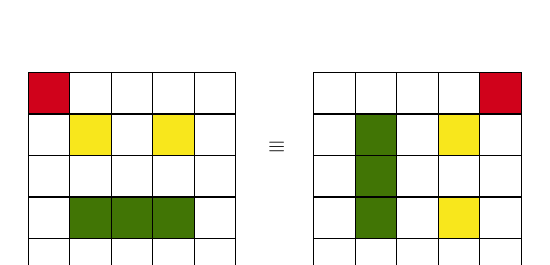
\begin{tikzpicture}[x=0.75pt,y=0.75pt,yscale=-1,xscale=1]
    %uncomment if require: \path (0,300); %set diagram left start at 0, and has height of 300
    
    %Shape: Rectangle [id:dp06222359392950061] 
    \draw  [draw opacity=0][fill={rgb, 255:red, 208; green, 2; blue, 27 }  ,fill opacity=1 ] (92.49,110) -- (112.49,110) -- (112.49,130) -- (92.49,130) -- cycle ;
    %Shape: Rectangle [id:dp8787181520000242] 
    \draw  [draw opacity=0][fill={rgb, 255:red, 248; green, 231; blue, 28 }  ,fill opacity=1 ] (112.49,130) -- (132.49,130) -- (132.49,150) -- (112.49,150) -- cycle ;
    %Shape: Rectangle [id:dp8843662801590229] 
    \draw  [draw opacity=0][fill={rgb, 255:red, 248; green, 231; blue, 28 }  ,fill opacity=1 ] (152.49,130) -- (172.49,130) -- (172.49,150) -- (152.49,150) -- cycle ;
    %Shape: Rectangle [id:dp594605756309508] 
    \draw  [draw opacity=0][fill={rgb, 255:red, 65; green, 117; blue, 5 }  ,fill opacity=1 ] (112.49,170) -- (132.49,170) -- (132.49,190) -- (112.49,190) -- cycle ;
    %Shape: Rectangle [id:dp4973176741292076] 
    \draw  [draw opacity=0][fill={rgb, 255:red, 65; green, 117; blue, 5 }  ,fill opacity=1 ] (132.49,170) -- (152.49,170) -- (152.49,190) -- (132.49,190) -- cycle ;
    %Shape: Rectangle [id:dp48750050163020564] 
    \draw  [draw opacity=0][fill={rgb, 255:red, 65; green, 117; blue, 5 }  ,fill opacity=1 ] (152.49,170) -- (172.49,170) -- (172.49,190) -- (152.49,190) -- cycle ;
    %Shape: Grid [id:dp38920287799224806] 
    \draw  [draw opacity=0] (92.49,110) -- (192.49,110) -- (192.49,210) -- (92.49,210) -- cycle ; \draw   (112.49,110) -- (112.49,210)(132.49,110) -- (132.49,210)(152.49,110) -- (152.49,210)(172.49,110) -- (172.49,210) ; \draw   (92.49,130) -- (192.49,130)(92.49,150) -- (192.49,150)(92.49,170) -- (192.49,170)(92.49,190) -- (192.49,190) ; \draw   (92.49,110) -- (192.49,110) -- (192.49,210) -- (92.49,210) -- cycle ;
    
    %Shape: Rectangle [id:dp07405696435517428] 
    \draw  [draw opacity=0][fill={rgb, 255:red, 208; green, 2; blue, 27 }  ,fill opacity=1 ] (330,110) -- (330,130) -- (310,130) -- (310,110) -- cycle ;
    %Shape: Rectangle [id:dp2999851790930883] 
    \draw  [draw opacity=0][fill={rgb, 255:red, 248; green, 231; blue, 28 }  ,fill opacity=1 ] (310,130) -- (310,150) -- (290,150) -- (290,130) -- cycle ;
    %Shape: Rectangle [id:dp3976751845049544] 
    \draw  [draw opacity=0][fill={rgb, 255:red, 248; green, 231; blue, 28 }  ,fill opacity=1 ] (310,170) -- (310,190) -- (290,190) -- (290,170) -- cycle ;
    %Shape: Rectangle [id:dp95157657313268] 
    \draw  [draw opacity=0][fill={rgb, 255:red, 65; green, 117; blue, 5 }  ,fill opacity=1 ] (270,130) -- (270,150) -- (250,150) -- (250,130) -- cycle ;
    %Shape: Rectangle [id:dp9173428399994787] 
    \draw  [draw opacity=0][fill={rgb, 255:red, 65; green, 117; blue, 5 }  ,fill opacity=1 ] (270,150) -- (270,170) -- (250,170) -- (250,150) -- cycle ;
    %Shape: Rectangle [id:dp878485319044743] 
    \draw  [draw opacity=0][fill={rgb, 255:red, 65; green, 117; blue, 5 }  ,fill opacity=1 ] (270,170) -- (270,190) -- (250,190) -- (250,170) -- cycle ;
    %Shape: Grid [id:dp8867295874263446] 
    \draw  [draw opacity=0] (330,110) -- (330,210) -- (230,210) -- (230,110) -- cycle ; \draw   (330,130) -- (230,130)(330,150) -- (230,150)(330,170) -- (230,170)(330,190) -- (230,190) ; \draw   (310,110) -- (310,210)(290,110) -- (290,210)(270,110) -- (270,210)(250,110) -- (250,210) ; \draw   (330,110) -- (330,210) -- (230,210) -- (230,110) -- cycle ;
    
    
    % Text Node
    \draw (207,142.4) node [anchor=north west][inner sep=0.75pt]  [xscale=0.8,yscale=0.8]  {$\equiv $};
    
    
    \end{tikzpicture}
    \]
\textit{Strategy}: Let \begin{itemize}[align=left]
    \item[$n_4$]: number of patterns with 4 equivalent forms, e.g. 
    \[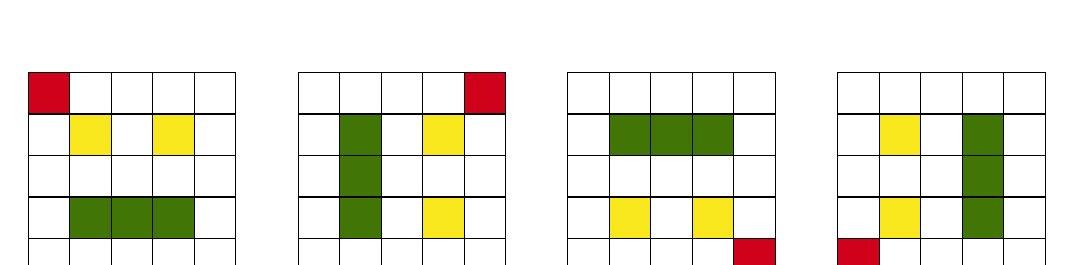
\begin{tikzpicture}[x=0.75pt,y=0.75pt,yscale=-1,xscale=1]
        %uncomment if require: \path (0,300); %set diagram left start at 0, and has height of 300
        
        %Shape: Rectangle [id:dp06222359392950061] 
        \draw  [draw opacity=0][fill={rgb, 255:red, 208; green, 2; blue, 27 }  ,fill opacity=1 ] (50,110) -- (70,110) -- (70,130) -- (50,130) -- cycle ;
        %Shape: Rectangle [id:dp8787181520000242] 
        \draw  [draw opacity=0][fill={rgb, 255:red, 248; green, 231; blue, 28 }  ,fill opacity=1 ] (70,130) -- (90,130) -- (90,150) -- (70,150) -- cycle ;
        %Shape: Rectangle [id:dp8843662801590229] 
        \draw  [draw opacity=0][fill={rgb, 255:red, 248; green, 231; blue, 28 }  ,fill opacity=1 ] (110,130) -- (130,130) -- (130,150) -- (110,150) -- cycle ;
        %Shape: Rectangle [id:dp594605756309508] 
        \draw  [draw opacity=0][fill={rgb, 255:red, 65; green, 117; blue, 5 }  ,fill opacity=1 ] (70,170) -- (90,170) -- (90,190) -- (70,190) -- cycle ;
        %Shape: Rectangle [id:dp4973176741292076] 
        \draw  [draw opacity=0][fill={rgb, 255:red, 65; green, 117; blue, 5 }  ,fill opacity=1 ] (90,170) -- (110,170) -- (110,190) -- (90,190) -- cycle ;
        %Shape: Rectangle [id:dp48750050163020564] 
        \draw  [draw opacity=0][fill={rgb, 255:red, 65; green, 117; blue, 5 }  ,fill opacity=1 ] (110,170) -- (130,170) -- (130,190) -- (110,190) -- cycle ;
        %Shape: Grid [id:dp38920287799224806] 
        \draw  [draw opacity=0] (50,110) -- (150,110) -- (150,210) -- (50,210) -- cycle ; \draw   (70,110) -- (70,210)(90,110) -- (90,210)(110,110) -- (110,210)(130,110) -- (130,210) ; \draw   (50,130) -- (150,130)(50,150) -- (150,150)(50,170) -- (150,170)(50,190) -- (150,190) ; \draw   (50,110) -- (150,110) -- (150,210) -- (50,210) -- cycle ;
        
        %Shape: Rectangle [id:dp07405696435517428] 
        \draw  [draw opacity=0][fill={rgb, 255:red, 208; green, 2; blue, 27 }  ,fill opacity=1 ] (280,110) -- (280,130) -- (260,130) -- (260,110) -- cycle ;
        %Shape: Rectangle [id:dp2999851790930883] 
        \draw  [draw opacity=0][fill={rgb, 255:red, 248; green, 231; blue, 28 }  ,fill opacity=1 ] (260,130) -- (260,150) -- (240,150) -- (240,130) -- cycle ;
        %Shape: Rectangle [id:dp3976751845049544] 
        \draw  [draw opacity=0][fill={rgb, 255:red, 248; green, 231; blue, 28 }  ,fill opacity=1 ] (260,170) -- (260,190) -- (240,190) -- (240,170) -- cycle ;
        %Shape: Rectangle [id:dp95157657313268] 
        \draw  [draw opacity=0][fill={rgb, 255:red, 65; green, 117; blue, 5 }  ,fill opacity=1 ] (220,130) -- (220,150) -- (200,150) -- (200,130) -- cycle ;
        %Shape: Rectangle [id:dp9173428399994787] 
        \draw  [draw opacity=0][fill={rgb, 255:red, 65; green, 117; blue, 5 }  ,fill opacity=1 ] (220,150) -- (220,170) -- (200,170) -- (200,150) -- cycle ;
        %Shape: Rectangle [id:dp878485319044743] 
        \draw  [draw opacity=0][fill={rgb, 255:red, 65; green, 117; blue, 5 }  ,fill opacity=1 ] (220,170) -- (220,190) -- (200,190) -- (200,170) -- cycle ;
        %Shape: Grid [id:dp8867295874263446] 
        \draw  [draw opacity=0] (280,110) -- (280,210) -- (180,210) -- (180,110) -- cycle ; \draw   (280,130) -- (180,130)(280,150) -- (180,150)(280,170) -- (180,170)(280,190) -- (180,190) ; \draw   (260,110) -- (260,210)(240,110) -- (240,210)(220,110) -- (220,210)(200,110) -- (200,210) ; \draw   (280,110) -- (280,210) -- (180,210) -- (180,110) -- cycle ;
        
        %Shape: Rectangle [id:dp1459753738426901] 
        \draw  [draw opacity=0][fill={rgb, 255:red, 208; green, 2; blue, 27 }  ,fill opacity=1 ] (410,210) -- (390,210) -- (390,190) -- (410,190) -- cycle ;
        %Shape: Rectangle [id:dp047714909261835414] 
        \draw  [draw opacity=0][fill={rgb, 255:red, 248; green, 231; blue, 28 }  ,fill opacity=1 ] (390,190) -- (370,190) -- (370,170) -- (390,170) -- cycle ;
        %Shape: Rectangle [id:dp7752200286439173] 
        \draw  [draw opacity=0][fill={rgb, 255:red, 248; green, 231; blue, 28 }  ,fill opacity=1 ] (350,190) -- (330,190) -- (330,170) -- (350,170) -- cycle ;
        %Shape: Rectangle [id:dp6751745224965142] 
        \draw  [draw opacity=0][fill={rgb, 255:red, 65; green, 117; blue, 5 }  ,fill opacity=1 ] (390,150) -- (370,150) -- (370,130) -- (390,130) -- cycle ;
        %Shape: Rectangle [id:dp8698376063283959] 
        \draw  [draw opacity=0][fill={rgb, 255:red, 65; green, 117; blue, 5 }  ,fill opacity=1 ] (370,150) -- (350,150) -- (350,130) -- (370,130) -- cycle ;
        %Shape: Rectangle [id:dp813968733924255] 
        \draw  [draw opacity=0][fill={rgb, 255:red, 65; green, 117; blue, 5 }  ,fill opacity=1 ] (350,150) -- (330,150) -- (330,130) -- (350,130) -- cycle ;
        %Shape: Grid [id:dp0328044922353814] 
        \draw  [draw opacity=0] (410,210) -- (310,210) -- (310,110) -- (410,110) -- cycle ; \draw   (390,210) -- (390,110)(370,210) -- (370,110)(350,210) -- (350,110)(330,210) -- (330,110) ; \draw   (410,190) -- (310,190)(410,170) -- (310,170)(410,150) -- (310,150)(410,130) -- (310,130) ; \draw   (410,210) -- (310,210) -- (310,110) -- (410,110) -- cycle ;
        
        %Shape: Rectangle [id:dp05493049941517203] 
        \draw  [draw opacity=0][fill={rgb, 255:red, 208; green, 2; blue, 27 }  ,fill opacity=1 ] (440,210) -- (440,190) -- (460,190) -- (460,210) -- cycle ;
        %Shape: Rectangle [id:dp9338392263695683] 
        \draw  [draw opacity=0][fill={rgb, 255:red, 248; green, 231; blue, 28 }  ,fill opacity=1 ] (460,190) -- (460,170) -- (480,170) -- (480,190) -- cycle ;
        %Shape: Rectangle [id:dp035596717155100155] 
        \draw  [draw opacity=0][fill={rgb, 255:red, 248; green, 231; blue, 28 }  ,fill opacity=1 ] (460,150) -- (460,130) -- (480,130) -- (480,150) -- cycle ;
        %Shape: Rectangle [id:dp7624099427520501] 
        \draw  [draw opacity=0][fill={rgb, 255:red, 65; green, 117; blue, 5 }  ,fill opacity=1 ] (500,190) -- (500,170) -- (520,170) -- (520,190) -- cycle ;
        %Shape: Rectangle [id:dp5363742427401106] 
        \draw  [draw opacity=0][fill={rgb, 255:red, 65; green, 117; blue, 5 }  ,fill opacity=1 ] (500,170) -- (500,150) -- (520,150) -- (520,170) -- cycle ;
        %Shape: Rectangle [id:dp1052878278253464] 
        \draw  [draw opacity=0][fill={rgb, 255:red, 65; green, 117; blue, 5 }  ,fill opacity=1 ] (500,150) -- (500,130) -- (520,130) -- (520,150) -- cycle ;
        %Shape: Grid [id:dp08023816682136653] 
        \draw  [draw opacity=0] (440,210) -- (440,110) -- (540,110) -- (540,210) -- cycle ; \draw   (440,190) -- (540,190)(440,170) -- (540,170)(440,150) -- (540,150)(440,130) -- (540,130) ; \draw   (460,210) -- (460,110)(480,210) -- (480,110)(500,210) -- (500,110)(520,210) -- (520,110) ; \draw   (440,210) -- (440,110) -- (540,110) -- (540,210) -- cycle ;
        
        
        
        
        
        \end{tikzpicture}
        \]
    \item[$n_2$]: number of patterns with 2 equivalent forms;
    \item[$n_1$]: number of patterns with 1 equivalent forms. 
\end{itemize}
\begin{itemize}
    \item Let $A_4$ be all patterns on a fixed board. Then $|A_4|=4^{25}$ and $|A_4|=4n_4+2n_2+n_1$. 

    \item Let $A_2$ be all patterns on a fixed board\sidenote{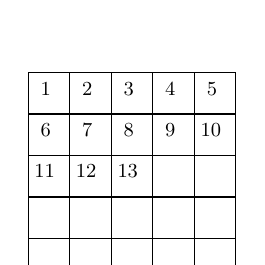
\begin{tikzpicture}[x=0.75pt,y=0.75pt,yscale=-1,xscale=1]
        %uncomment if require: \path (0,300); %set diagram left start at 0, and has height of 300
        
        
        %Shape: Grid [id:dp2046265074316873] 
        \draw  [draw opacity=0] (70,107.62) -- (170,107.62) -- (170,207.62) -- (70,207.62) -- cycle ; \draw   (90,107.62) -- (90,207.62)(110,107.62) -- (110,207.62)(130,107.62) -- (130,207.62)(150,107.62) -- (150,207.62) ; \draw   (70,127.62) -- (170,127.62)(70,147.62) -- (170,147.62)(70,167.62) -- (170,167.62)(70,187.62) -- (170,187.62) ; \draw   (70,107.62) -- (170,107.62) -- (170,207.62) -- (70,207.62) -- cycle ;
        
        % Text Node
        \draw (75,111.4) node [anchor=north west][inner sep=0.75pt]  [font=\small,xscale=0.8,yscale=0.8]  {$1$};
        % Text Node
        \draw (95,111.4) node [anchor=north west][inner sep=0.75pt]  [font=\small,xscale=0.8,yscale=0.8]  {$2$};
        % Text Node
        \draw (115,111.4) node [anchor=north west][inner sep=0.75pt]  [font=\small,xscale=0.8,yscale=0.8]  {$3$};
        % Text Node
        \draw (135,111.4) node [anchor=north west][inner sep=0.75pt]  [font=\small,xscale=0.8,yscale=0.8]  {$4$};
        % Text Node
        \draw (155,111.4) node [anchor=north west][inner sep=0.75pt]  [font=\small,xscale=0.8,yscale=0.8]  {$5$};
        % Text Node
        \draw (75,131.4) node [anchor=north west][inner sep=0.75pt]  [font=\small,xscale=0.8,yscale=0.8]  {$6$};
        % Text Node
        \draw (95,131.4) node [anchor=north west][inner sep=0.75pt]  [font=\small,xscale=0.8,yscale=0.8]  {$7$};
        % Text Node
        \draw (115,131.4) node [anchor=north west][inner sep=0.75pt]  [font=\small,xscale=0.8,yscale=0.8]  {$8$};
        % Text Node
        \draw (135,131.4) node [anchor=north west][inner sep=0.75pt]  [font=\small,xscale=0.8,yscale=0.8]  {$9$};
        % Text Node
        \draw (152,131.02) node [anchor=north west][inner sep=0.75pt]  [font=\small,xscale=0.8,yscale=0.8]  {$10$};
        % Text Node
        \draw (72,151.02) node [anchor=north west][inner sep=0.75pt]  [font=\small,xscale=0.8,yscale=0.8]  {$11$};
        % Text Node
        \draw (92,151.02) node [anchor=north west][inner sep=0.75pt]  [font=\small,xscale=0.8,yscale=0.8]  {$12$};
        % Text Node
        \draw (112,151.02) node [anchor=north west][inner sep=0.75pt]  [font=\small,xscale=0.8,yscale=0.8]  {$13$};
        
        
        \end{tikzpicture}
        } that are symmetric when rotated 180º. Then $|A_2|=4^{13}$ and $|A_2|=2n_2+n_1$.

        \item Let $A_2$ be all patterns on a fixed board\sidenote{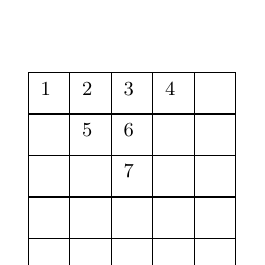
\begin{tikzpicture}[x=0.75pt,y=0.75pt,yscale=-1,xscale=1]
            %uncomment if require: \path (0,300); %set diagram left start at 0, and has height of 300
            
            
            %Shape: Grid [id:dp2046265074316873] 
            \draw  [draw opacity=0] (70,107.62) -- (170,107.62) -- (170,207.62) -- (70,207.62) -- cycle ; \draw   (90,107.62) -- (90,207.62)(110,107.62) -- (110,207.62)(130,107.62) -- (130,207.62)(150,107.62) -- (150,207.62) ; \draw   (70,127.62) -- (170,127.62)(70,147.62) -- (170,147.62)(70,167.62) -- (170,167.62)(70,187.62) -- (170,187.62) ; \draw   (70,107.62) -- (170,107.62) -- (170,207.62) -- (70,207.62) -- cycle ;
            
            % Text Node
            \draw (75,111.4) node [anchor=north west][inner sep=0.75pt]  [font=\small,xscale=0.8,yscale=0.8]  {$1$};
            % Text Node
            \draw (95,111.4) node [anchor=north west][inner sep=0.75pt]  [font=\small,xscale=0.8,yscale=0.8]  {$2$};
            % Text Node
            \draw (115,111.4) node [anchor=north west][inner sep=0.75pt]  [font=\small,xscale=0.8,yscale=0.8]  {$3$};
            % Text Node
            \draw (135,111.4) node [anchor=north west][inner sep=0.75pt]  [font=\small,xscale=0.8,yscale=0.8]  {$4$};
            % Text Node
            % \draw (155,111.4) node [anchor=north west][inner sep=0.75pt]  [font=\small,xscale=0.8,yscale=0.8]  {$5$};
            % Text Node
            % \draw (75,131.4) node [anchor=north west][inner sep=0.75pt]  [font=\small,xscale=0.8,yscale=0.8]  {$6$};
            % Text Node
            \draw (95,131.4) node [anchor=north west][inner sep=0.75pt]  [font=\small,xscale=0.8,yscale=0.8]  {$5$};
            % Text Node
            \draw (115,131.4) node [anchor=north west][inner sep=0.75pt]  [font=\small,xscale=0.8,yscale=0.8]  {$6$};
            % Text Node
            % \draw (135,131.4) node [anchor=north west][inner sep=0.75pt]  [font=\small,xscale=0.8,yscale=0.8]  {$9$};
            % Text Node
            % \draw (152,131.02) node [anchor=north west][inner sep=0.75pt]  [font=\small,xscale=0.8,yscale=0.8]  {$10$};
            % Text Node
            % \draw (72,151.02) node [anchor=north west][inner sep=0.75pt]  [font=\small,xscale=0.8,yscale=0.8]  {$11$};
            % Text Node
            % \draw (92,151.02) node [anchor=north west][inner sep=0.75pt]  [font=\small,xscale=0.8,yscale=0.8]  {$12$};
            % Text Node
            \draw (115,151.02) node [anchor=north west][inner sep=0.75pt]  [font=\small,xscale=0.8,yscale=0.8]  {$7$};
            
            
            \end{tikzpicture}
            } that are symmetric when rotated 90º. Then $|A_2|=4^{7}$ and $|A_1|=n_1$.
\end{itemize}

Thus: \begin{align*}
    4n_4+2n_2+n_1&=4^{25}\\
    2n_2+n_1&=4^{13}\\
    n_1&=4^{7}\\
\end{align*}
So we write \[\begin{bmatrix}
    4&2&1\\0&2&1\\0&0&1
\end{bmatrix}\cdot \begin{bmatrix}
    n_4\\n_2\\n_1
\end{bmatrix} = \begin{bmatrix}
    4^{25}\\4^{13}\\4^{7}
\end{bmatrix}\]
Notice that\sidenote{note the RHS represents $n_1+n_2+n_4$} \[\frac{1}{4}\begin{bmatrix}
    1&1&2
\end{bmatrix}\begin{bmatrix}
    4&2&1\\0&2&1\\0&0&1
\end{bmatrix} =  \begin{bmatrix}
    1&1&1
\end{bmatrix}\]
Solve for LHS and we are done.

\eg How many ways too place plates of $a$ colors on a circular table with 6 places, up to rotational equivalece?

Let $n_k$ be the number of such arrangements that have $k$ vertices on a fixed table. Then $ANS=n_6+n_3+n_2+n_1$. Now: \begin{itemize}
    \item $|A_6|=a^6=6n_6+3n_3+2n_2+n_1$
    \item $|A_3|=a^3=3n_3+n_1$
    \item $|A_2|=a^2=2n_2+n_1$
    \item $|A_1|=a=n_1$
\end{itemize}
So we write \[\begin{bmatrix}
    6&3&2&1\\0&3&0&1\\0&0&0&1
\end{bmatrix}\cdot \begin{bmatrix}
    n_6\\n_3\\n_2\\n_1
\end{bmatrix} = \begin{bmatrix}
    a^6\\a^3\\a^2\\a
\end{bmatrix}\]
Notice that\sidenote{note the RHS represents $n_1+n_2+n_4$} \[\frac{1}{6}\begin{bmatrix}
    1&1&2&2
\end{bmatrix}\begin{bmatrix}
    6&3&2&1\\0&3&0&1\\0&0&0&1
\end{bmatrix} =  \begin{bmatrix}
    1&1&1&1
\end{bmatrix}\]
Solve for LHS: \[ANS = \frac{1}{6}\begin{bmatrix}
    1&1&2&2
\end{bmatrix}\begin{bmatrix}
    a^6\\a^3\\a^2\\a
\end{bmatrix} = \frac{a^6+a^3+2a^2+2a}{6}\]

\subsection{K2 Group actions on sets}
Both of the problems above are about counting \textbf{orbits} of a group action. We look at actions of group $G$ on a set $X$. 

\eg $G=\znz{4}$ and $X$ be the set of colorings/patterns in 4 colors of a $5\times 5$ chessboard. We ``relabel'' the group elements as $\{R_0, R_{90}, R_{180}, R_{270}\}$ where $R_k$ is rotation by $k$ degrees. Then the group action $R_k\cdot x$ would just be taking a coloring $x\in X$ and rotate it by $k$º. The \textbf{orbits} are the equivalence classes under the group action.

\eg Visually, let $G=\{0,\rt{1},2\}$ be a cyclic group of order 3 under + and let $X$ be the set: \sidenote{the actions corresponding to 2 are just those of \rt{1} in reverse direction due to 2 being the inverse of 1}
\[\begin{tikzcd}[ampersand replacement=\&,cramped,sep=scriptsize]
	\&\&\&\& \bullet \\
	\bullet \& \bullet \&\& \bullet \\
	\&\& \bullet \&\& \bullet \\
	\& \bullet \&\& \bullet
	\arrow[color=magenta, from=1-5, to=2-4]
	\arrow[color=magenta, from=2-1, to=2-2]
	\arrow[color=magenta, from=2-2, to=3-3]
	\arrow[color=magenta, from=3-3, to=2-1]
	\arrow[color=magenta, from=3-5, to=1-5]
	\arrow[color=magenta, from=3-5, to=2-4]
	\arrow[color=magenta, from=4-2, to=4-2, loop, in=55, out=125, distance=10mm]
	\arrow[color=magenta, from=4-4, to=4-4, loop, in=55, out=125, distance=10mm]
\end{tikzcd}\]
We observe that we have 4 \textbf{orbits}.

\begin{theorem}
    Let $G=\znz{3}$ act on a \textbf{finite} set $X$. Then $X$ is \textbf{partitioned} into orbits of size 3 and orbits of size 1. That is, \[|X|\equiv \underbrace{|\text{orbits of size 1}|}_{|X^G|} \mod 3\]
    where $X^G$ is the set of \textbf{fixed points} of the action.
\end{theorem}
\begin{proof}
    For each $x\in X$, \begin{itemize}[align=left]
        \item[\textbf{Either:}] $\rt{1}\cdot x=x$
        
        Then $2x = \rt{1}(\rt{1}x) = \rt{1}\cdot x = x$ and so $x$ is \textbf{completely} fixed by the group action. This means the orbit of $x$ has size 1.

        \item[\textbf{Or:}]  $\rt{1}\cdot x = x'\neq x$
        
        Then claim that $x'' = 2\cdot x $ is distinct from $x$ and $x'$. This is because if $2x=x$, then $\rt{1}\cdot 2x = 1\cdot x = x$ resulting in a contradiction of $x=x'$. Similarly, if $2x = \rt{1}x$, then $2\cdot 2x = 2\cdot \rt{1}x$  resulting in a contradiction of $x'=x$. 

        Thus, orbit of this $x$ must have size 3.
    \end{itemize}
\end{proof}

\section{K3 Stabilizers}
\defn[Stabilizer of $x$] For any $x\in X$, define \[G_x = \operatorname*{Stab}(x) = \{g\in G \mid g\cdot x = x\}\]
That is, all elements that would fix the particular $x$ when acting on it.

\eg Let $G=\znz{6}$.
\[\input{Images/tables_stab.svg.pdf_tex}\]

\begin{theorem}
    Stab$(x)$ is a subgroup of $G$.
\end{theorem}

\addlink{Orbit-stabilizer theorem}
\begin{theorem}[Orbit-stabilizer]
    If $G$ is a finite group acting on a set $X$, then \[|\operatorname*{Orbit}(x)||G_x|=|G|\]
    for all $x\in X$.
\end{theorem}
\begin{proof}[Proof omitted, just see abstract alg. notes]
\end{proof}

\subsection{K4 Fixed points}
Let $G$ act on $X$. For all $g\in G$, define \[X^g = \{x\in X\mid g\cdot x= x\}\]
i.e. the set of the elements fixed by $g$.

Define $$X^G = \bigcap_{g\in G}x^g$$ to be the fixed point set of the action, i.e. the set of elements that are fixed by any $g$.

\eg Let $G= \znz{6}$ and $X$ be the set of patterns of plates on a table for 6. Let $g=2$. Then \[X^g =\{\text{tables in the form of }(ababab)\}\]
where $a,b$ aren't necessarily distinct. Moreover, \[X^G = \{\text{monochromatic tables}\}\]

\theorem \label[theorem]{fixed-points-stab}\[\sum_{x\in X}|G^x| = \sum_{g\in G}|X^g|\]
\begin{proof}
    Both are equal to \[\left|\left\{(x,g)\mid g\cdot x = x\right\}\subseteq X\times G\right|\]
\end{proof}

\subsection{K5 Burnside's lemma}
\begin{lemma}[Burnside's]
    Let $G$ be a finite group acting on finite set $X$. Then the number of the orbits are the \pt{average number of fixed points} of the elements of $G$: \sidenote{\pt{$X/G$} is the set of orbits}\[\# \text{ Orbits}  = \pt{|X/G|}= \frac{1}{|G|}\sum_{g\in G}|X^{g}|\]
\end{lemma}
\begin{proof}
    Let $B$ denote orbits.
    \begin{align*}
        |X/G| &= \sum_{B\in X/G}1\\
        &= \sum_{B\in X/G}\sum_{x\in B}\frac{1}{|B|}\\
        &= \sum_{x\in X}\frac{1}{|\operatorname*{orbit}(x)|}\\
        &= \sum_{x\in X}\frac{|G_x|}{|G|} && \text{by O-S thm.}\\
        &= \frac{1}{|G|}\sum_{x\in X}|G_x|\\
        &= \frac{1}{|G|}\sum_{g\in G}|X^{g}| && \text{by \cref{fixed-points-stab}}
    \end{align*}
\end{proof}

\eg Recall Investigation 7: \textit{A dinner party host has unlimited numbers of plates in $a$ different colours.
How many distinguishable arrangements of coloured plates are there at a circular table with
6 equally-spaced seats? }

Let $G=\znz{6}$, $X$ be the arrangements on a fixed table. We calculate: \begin{align*}
    |X/G| &= \frac{1}{|G|}\left(x^0+x^1+x^2+x^3+x^4+x^5\right)\\
    &= \frac{1}{6}(a^6+a+a^2+a^3+a^2+a)\\
    &= \frac{a^6+a^3+2a^2+2a}{6}
\end{align*}

\end{document}